\documentclass{frama-c-book}

\usepackage{microtype}
\usepackage{lmodern}
\usepackage{booktabs}
\usepackage{calc}
\usepackage{multirow}

%%%%%%%%%%%%%%%%%%%%%%%%%%%%%%%%%%%%%%%%%%%%%%%%%%%%%%%%%%%%%%%%%%%%%%%%%%%%%%%%
% Date
%%%%%%%%%%%%%%%%%%%%%%%%%%%%%%%%%%%%%%%%%%%%%%%%%%%%%%%%%%%%%%%%%%%%%%%%%%%%%%%%

% Useful for today's short date
\def\shorttoday{\leavevmode\hbox{\the\year-\twodigits\month-\twodigits\day}}
\def\twodigits#1{\ifnum#1<10 0\fi\the#1}

%%%%%%%%%%%%%%%%%%%%%%%%%%%%%%%%%%%%%%%%%%%%%%%%%%%%%%%%%%%%%%%%%%%%%%%%%%%%%%%%
% Indexed Keywords
%%%%%%%%%%%%%%%%%%%%%%%%%%%%%%%%%%%%%%%%%%%%%%%%%%%%%%%%%%%%%%%%%%%%%%%%%%%%%%%%

% Frama-C plug-in names (e.g., \plugin{Eva})
\newcommand{\plugin}[1]{\textsf{#1}\xspace}

% Tools (e.g., \tool{Why3})
\newcommand{\tool}[1]{\textsf{#1}\xspace}

% Languages (e.g., \lang{ACSL}, \lang{C})
\newcommand{\lang}[1]{\textsf{#1}\xspace}

% Libraries (e.g., \library{Gmp})
\newcommand{\library}[1]{\textsf{#1}\xspace}

% Benchmarks (e.g, \benchmark{SpecCPU})
\newcommand{\benchmark}[1]{\textsf{#1}\xspace}

%%%%%%%%%%%%%%%%%%%%%%%%%%%%%%%%%%%%%%%%%%%%%%%%%%%%%%%%%%%%%%%%%%%%%%%%%%%%%%%%
% Frama-C Related Names
%%%%%%%%%%%%%%%%%%%%%%%%%%%%%%%%%%%%%%%%%%%%%%%%%%%%%%%%%%%%%%%%%%%%%%%%%%%%%%%%

\newcommand{\FramaC}{\tool{Frama-C}}
\newcommand{\acsl}{\lang{ACSL}}
\newcommand{\eacsllang}{\lang{E-ACSL}}

% plug-ins
\newcommand{\aorai}{\plugin{Aora\"i}}
\newcommand{\cafe}{\plugin{CaFE}}
\newcommand{\callgraph}{\plugin{Callgraph}}
\newcommand{\constfold}{\plugin{Consfold}}
\newcommand{\dive}{\plugin{Dive}}
\newcommand{\dominators}{\plugin{Dominators}}
\newcommand{\eacsl}{\plugin{E-ACSL}}
\newcommand{\Eva}{\plugin{Eva}}
\newcommand{\framaclang}{\plugin{Frama-Clang}}
\newcommand{\from}{\plugin{From}}
\newcommand{\GUI}{\plugin{GUI}}
\newcommand{\impact}{\plugin{Impact}}
\newcommand{\inout}{\plugin{InOut}}
\newcommand{\instantiate}{\plugin{Instantiate}}
\newcommand{\ltest}{\plugin{LTest}}
\newcommand{\mdr}{\plugin{MdR}}
\newcommand{\metacsl}{\plugin{MetAcsl}}
\newcommand{\metrics}{\plugin{Metrics}}
\newcommand{\nonterm}{\plugin{NonTerm}}
\newcommand{\obfuscator}{\plugin{Obfuscator}}
\newcommand{\occurrence}{\plugin{Occurrence}}
\newcommand{\pathcrawler}{\plugin{PathCrawler}}
\newcommand{\pdg}{\plugin{Pdg}}
\newcommand{\pilat}{\plugin{Pilat}}
\newcommand{\postdominators}{\plugin{Postdominators}}
\newcommand{\printinterface}{\plugin{PrintInterface}}
\newcommand{\reduction}{\plugin{Reduction}}
\newcommand{\report}{\plugin{Report}}
\newcommand{\rpp}{\plugin{RPP}}
\newcommand{\rte}{\plugin{Rte}}
\newcommand{\scope}{\plugin{Scope}}
\newcommand{\secureflow}{\plugin{SecureFlow}}
\newcommand{\securityslicing}{\plugin{SecuritySlicing}}
\newcommand{\server}{\plugin{Server}}
\newcommand{\slicing}{\plugin{Slicing}}
\newcommand{\sparecode}{\plugin{SpareCode}}
\newcommand{\stady}{\plugin{StaDy}}
\newcommand{\studia}{\plugin{Studia}}
\newcommand{\users}{\plugin{Users}}
\newcommand{\variadic}{\plugin{Variadic}}
\newcommand{\Wp}{\plugin{WP}}

%%%%%%%%%%%%%%%%%%%%%%%%%%%%%%%%%%%%%%%%%%%%%%%%%%%%%%%%%%%%%%%%%%%%%%%%%%%%%%%%
% Standard Keywords
%%%%%%%%%%%%%%%%%%%%%%%%%%%%%%%%%%%%%%%%%%%%%%%%%%%%%%%%%%%%%%%%%%%%%%%%%%%%%%%%

% Some programming languages
\newcommand{\ada}{\lang{Ada}}
\newcommand{\awk}{\lang{Awk}}
\newcommand{\C}{\lang{C}}
\newcommand{\coq}{\lang{Coq}}
\newcommand{\Cpp}{\lang{C++}}
\newcommand{\csharp}{\lang{C\#}}
\newcommand{\dafny}{\lang{Dafny}}
\newcommand{\dotnet}{\lang{.NET}}
\newcommand{\eiffel}{\lang{Eiffel}}
\newcommand{\fortran}{\lang{Fortran}}
\newcommand{\isabelle}{\lang{Isabelle}}
\newcommand{\java}{\lang{Java}}
\newcommand{\javacard}{\lang{JavaCard}}
\newcommand{\K}{\ensuremath{\mathbb{K}}}
\newcommand{\ocaml}{\lang{OCaml}}
\newcommand{\php}{\lang{PHP}}
\newcommand{\python}{\lang{Python}}
\newcommand{\smalltalk}{\lang{Smalltalk}}
\newcommand{\spark}{\lang{Spark2014}}
\newcommand{\vbnet}{\lang{VB.NET}}

% Some modeling languages
\newcommand{\lustre}{\lang{Lustre}}
\newcommand{\scade}{\lang{Scade}}
\newcommand{\simulink}{\lang{Simulink}}

% Some specification languages
\newcommand{\codecontract}{\lang{Code Contract}}
\newcommand{\ltl}{\lang{LTL}}
\newcommand{\jml}{\lang{JML}}
\newcommand{\specsharp}{\lang{Spec\#}}
\newcommand{\vcc}{\lang{VCC}}

% Some libraries
\newcommand{\cil}{\library{Cil}}
\newcommand{\gtk}{\library{Gtk2}}
\newcommand{\gtkt}{\library{Gtk3}}
\newcommand{\gmp}{\library{Gmp}}
\newcommand{\lablgtk}{\library{LablGtk2}}
\newcommand{\lablgtkt}{\library{LablGtk3}}
\newcommand{\libc}{\library{libc}}
\newcommand{\libtomcrypt}{\library{LibTomCrypt}}

% Some analysis and verification tools
\newcommand{\addresssanitizer}{\tool{AddressSanitizer}}
\newcommand{\aiT}{\tool{aiT}}
\newcommand{\astree}{\tool{Astr\'ee}}
\newcommand{\caduceus}{\tool{Caduceus}}
\newcommand{\drmemory}{\tool{Dr.~Memory}}
\newcommand{\insurepp}{\tool{Insure++}}
\newcommand{\memcheck}{\tool{MemCheck}}
\newcommand{\memorysanitizer}{\tool{MemorySanitizer}}
\newcommand{\memsanitizer}{\tool{MemorySanitizer}}
\newcommand{\openjml}{\tool{OpenJML}}
\newcommand{\polyspace}{\tool{PolySpace}}
\newcommand{\purify}{\tool{Purify}}
\newcommand{\rvmatch}{\tool{RV-Match}}
\newcommand{\stackanalyzer}{\tool{Stackanalyzer}}
\newcommand{\threadsanitizer}{\tool{ThreadSanitizer}}
\newcommand{\undefsanitizer}{\tool{UndefinedBehaviorSanitizer}}
\newcommand{\valgrind}{\tool{Valgrind}}
\newcommand{\verasco}{\tool{Verasco}}
\newcommand{\why}{\tool{Why}}
\newcommand{\whyt}{\tool{Why3}}

% Some other tools
\newcommand{\altergo}{\tool{Alt-Ergo}}
\newcommand{\clang}{\tool{Clang}}
\newcommand{\clousot}{\tool{Clousot}}
\newcommand{\compcert}{\tool{CompCert}}
\newcommand{\gcc}{\tool{Gcc}}
\newcommand{\gdb}{\tool{gdb}}
\newcommand{\git}{\tool{Git}}
\newcommand{\llvm}{\tool{LLVM}}
\newcommand{\opam}{\tool{opam}}


% Commandes pour mettre des ref dans l'index :
\newcommand{\idb}[1]{\textbf{#1}}
\newcommand{\indextxt}[1]{\index{#1}{\bf #1}}
\newcommand{\indexdef}[1]{\index{#1|idb}{{\bf #1}}}
\newcommand{\indextxtdef}[2]{\index{#2|idb}{{\bf #1}}}

\renewcommand{\labelitemii}{$\triangleright$}

\newcommand{\bropen}{\mbox{\tt [}}
\newcommand{\brclose}{\mbox{\tt ]}}
\newcommand{\cbopen}{\mbox{\tt \{}}
\newcommand{\cbclose}{\mbox{\tt \}}}

\newcommand{\framacversion}%
           {\input{../../VERSION} (\input{../../VERSION_CODENAME}\unskip)}
\newcommand{\isoc}{\textsf{C99}}

\lstset{literate=%
{∈}{{$\in$ }}1
}

\title{The \Eva{} plug-in}
\author{David Bühler, Pascal Cuoq and Boris Yakobowski. \\
With Matthieu Lemerre, André Maroneze,
Valentin Perrelle and Virgile Prevosto}

\fcversion{\framacversion}

\cclicence{by-sa}
\copyrightstarts{2011}

%==============================================================================
\begin{document}
\sloppy
\emergencystretch 3em

\maketitle
\tableofcontents

\chapter*{Foreword}
\markright{}
\addcontentsline{toc}{chapter}{Foreword}

This is the documentation of the \FramaC plug-in \Eva.

The content of this document corresponds to the version \framacversion, released
on \today, of \FramaC. However the development of \FramaC is still ongoing:
features described here may still evolve in the future.

\section*{Acknowledgements}
%\addcontentsline{toc}{chapter}{Acknowledgements}

\medskip

\acknowledgeANR{
the French ANR projects U3CAT~(08-SEGI-021-01)
}

\chapter{Introduction}\label{introduction}
\vspace{2cm}

{\em Frama-C is a modular static analysis framework for the C language.\\
This manual documents the \Eva{} (for \emph{Evolved Value Analysis}) plug-in of Frama-C.}
\vspace{2cm}

The \Eva{} plug-in automatically computes sets of possible
values for the variables of an analyzed program. \Eva{}
warns about possible run-time errors in the analyzed program.
Lastly, synthetic information
about each analyzed function can be computed automatically from the
values provided by \Eva{}: these functionalities (input
variables, output variables, and information flow) are also documented
here.  \bigskip

The framework, the \Eva{} plug-in and the other plug-ins
documented here are all Open Source software. They can be
downloaded from \url{http://frama-c.com/}.
\bigskip

In technical terms, \Eva{} is context-sensitive and
path-sensitive. In non-technical terms, this means that it tries to
offer precise results for a large set of C programs. Heterogeneous
pointer casts, function pointers, and floating-point computations are
handled.

\section{First contact}
Frama-C comes with two interfaces: batch and interactive.
The interactive graphical interface of Frama-C displays
a normalized version of the analyzed source code.
In this interface, the \Eva{} plug-in allows the user
to select an expression in the
code and observe an over-approximation of the set of
values this expression can take at run-time.

Here is a simple C example:
\listinginputcaption{1}{\texttt{introduction.c}}{examples/introduction.c}

If either interface of Frama-C is launched with options
\lstinline|-eva introduction.c|,
the \Eva{} plug-in is able to guarantee that at each passage through
the \lstinline|return| statement of
function \lstinline|f|, the global variables \lstinline+y+ and
\lstinline+z+ each contain either 1 or 3.
At the end of function  \lstinline|main|,
it indicates that  \lstinline|y|
necessarily contains  4, and the value of  \lstinline|z| is again 1 or 3.

When the plug-in indicates the value of \lstinline|y| is 1 or 3
at the end of function \lstinline|f|, it implicitly computes the union
of all the values in \lstinline|y|
at each passage through this program point throughout any execution.
In an actual execution of this deterministic program,
there is only one passage though the end
of function  \lstinline|main|, and therefore only one value for \lstinline|z|
at this point.
The answer given by \Eva{} is approximated but correct (the actual
value, 3, is among the proposed values).

The theoretical framework on which \Eva{} is founded is called
Abstract Interpretation and has been the subject of extensive research
during the last forty years.

\section{Run-time errors and the absence thereof}

An analyzed application may contain run-time errors: divisions by zero,
invalid pointer accesses,\ldots

\listinginputcaption{1}{\texttt{rte.c}}{examples/rte.c}

When launched with \lstinline|frama-c -eva rte.c|,
\Eva{} emits a warning about an out-of-bound access at line 5:
\begin{logs}
[eva:alarm] rte.c:5: Warning: accessing out of bounds index. assert i < 10;
\end{logs}
There is in fact an out-of-bounds access at this line in the program.
It can also happen that, because of approximations during its computations,
Frama-C emits warnings for constructs
that do not cause any run-time errors. These are called ``false alarms''.
On the other hand, the fact that \Eva{}
computes correct, over-approximated sets of possible values prevents it
from remaining silent on a program that contains a run-time error. For
instance, a particular division in the analyzed program
is the object of a warning
as soon as the set of possible values for the divisor
contains zero. Only
if the set of possible values computed by \Eva{}
does not contain zero is the warning omitted, and
that means that the divisor really cannot be null at run-time.

\section{From Value Analysis to \Eva{}}

The \Eva{} plug-in was previously called the \emph{Value Analysis plug-in}.
Following major changes in its expressivity and overall precision,
the plugin was subsequently renamed to \emph{Evolved Value Analysis}, or
\Eva{} for short. Those changes were first made available with the
Aluminium version of Frama-C. They are presented in section~\ref{sec:eva}.

\section{Other analyses based on \Eva{}}

Frama-C also provides
synthetic information on the behavior of analyzed functions:
inputs, outputs, and dependencies. This information is computed
from the results of the \Eva{} plug-in,
and therefore some familiarity with \Eva{}
is necessary to get the most of these computations.

\chapter{Tutorial}\label{tutorial}
\vspace{2cm}

{\em Some use cases for \Eva{}\ldots}

\vspace{2cm}

\section{Introduction}

Throughout this tutorial, we will see on a single example how to use
\Eva{} for the following tasks :
\begin{enumerate}
\item to get familiar with foreign code,
\item to produce documentation automatically,
\item to search for bugs,
\item to guarantee the absence of bugs.
\end{enumerate}
It is useful to stick to a single example in this tutorial, and
there is a natural progression to the list of results above,
but in real life, a single person would generally focus on
only one or two of these four tasks for a given
codebase. For instance, if you need Frama-C's help to reverse
engineer the code as in tasks 1 and 2, you have
probably not been provided with the quantity of documentation
and specifications
that is appropriate for meaningfully carrying out task 4.

Frama-C helps you to achieve tasks 1-3 in less time than you would
need to get the same results using the traditional approach of writing
tests cases. Task 4, formally guaranteeing the absence of bugs, can in
the strictest sense not be achieved at all using tests for two
reasons.  Firstly, many forms of bugs that occur in a C program
(including buffer overflows) may cause the behavior of the program to
be non-deterministic.  As a consequence, even when a test suite comes
across a bug, the faulty program may appear to work correctly during
tests and fail later, after it has been deployed.  Secondly, the
notion of coverage of a test suite in itself is an invention made
necessary because tests aren't usually exhaustive.  Assume a
function's only inputs are two 32-bit integers, each allowed to take
the full range of their possible values.  Further assume that this
function only takes a billionth of a second to run (a couple of cycles
on a 2GHz processor).  A pencil and the back of an envelope show that
this function would take 600 years to test exhaustively.  Testing
coverage criteria can help decide a test suite is ``good enough'', but
there is an implicit assumption in this reasoning.  The assumption is
that a test suite that satisfies the coverage criteria finds all the
bugs that need to be found, and this assumption is justified
empirically only.

\section{Target code: Skein-256}

A single piece of code, the reference implementation for the Skein
hash function, is used as an example throughout this document. As of
this writing, this implementation is available at
\url{http://www.schneier.com/code/skein.zip}. The Skein function is
Niels Ferguson, Stefan Lucks, Bruce Schneier, Doug Whiting, Mihir
Bellare, Tadayoshi Kohno, Jon Callas, and Jesse Walker's entry in the
NIST cryptographic hash algorithm competition for SHA-3.

Cryptographic hash functions are one of the basic building blocks from
which cryptographic protocols are designed. Many cryptographic
protocols are designed with the assumption that an implementation for
a function $h$ from strings to fixed-width integers is available with
the following two properties:
\begin{itemize}
\item it is difficult to find two distinct, arbitrary strings $s_1$ and $s_2$
such that $h(s_1)=h(s_2)$,
\item for a given integer $i$, it is difficult to build a string $s$
such that $h(s)=i$.
\end{itemize}
A function with the above two properties is called a cryptographic hash
function. It is of the utmost importance that the function actually
chosen in the implementation of a cryptographic application satisfies the
above properties! Any weakness in the hash function can be
exploited to corrupt the application.

Proofs of security for
cryptographic hash functions are complicated mathematical affairs.
These proofs are made using a mathematical definition
of the function. Using static analysis for verifying that a piece
of code corresponds to the mathematical model
which was the object of the security proofs is an interesting
topic but is outside the scope of this tutorial.
In this document, we will not  be using \Eva{} for
verifying cryptographic properties.

We will, however, use \Eva{} to familiarize ourselves
with Skein's reference implementation, and we will see that
it can be a more useful tool than, say, a C
compiler, to this effect. We will also use \Eva{} to look
for bugs in the implementation of Skein, and finally prove that the
functions that implement Skein may never cause a run-time error for a
general use pattern. Because of the numerous pitfalls of the C
programming language, any amount of work at the
mathematical level cannot exclude the possibility of problems
such as buffer overflows in the implementation.
It is a good thing to be able to rule these out with \Eva{}.

\Eva{} is most useful for embedded or embedded-like
code. Although the Skein library does not exactly fall in this category,
it does not demand dynamic allocation and uses few functions from external
libraries, so it is well suited to this analysis.

\section{Using \Eva{} for getting familiar with Skein}

\subsection{Writing a test}

After extracting the archive \lstinline|skein_NIST_CD_010509.zip|,
listing the files in\\
\lstinline|NIST/CD/Reference_Implementation| shows:
\begin{listing-nonumber}
SHA3api_ref.c
SHA3api_ref.h
brg_endian.h
brg_types.h
skein.c
skein.h
skein_block.c
skein_debug.c
skein_debug.h
skein_port.h
\end{listing-nonumber}

The most natural place to go next is the file \lstinline|skein.h|,
since its name hints that this is the header with the
function declarations that should be called from outside the library.
Scanning the file quickly, we may notice declarations such as
\begin{listing-nonumber}
typedef struct /*  256-bit Skein hash context structure */
    {
      [...]
    } Skein_256_Ctxt_t;

/*   Skein APIs for (incremental) "straight hashing" */
int  Skein_256_Init  (Skein_256_Ctxt_t *ctx, size_t hashBitLen);
[...]
int  Skein_256_Update(Skein_256_Ctxt_t *ctx, const u08b_t *msg,
                                                 size_t msgByteCnt);
[...]
int  Skein_256_Final (Skein_256_Ctxt_t *ctx, u08b_t * hashVal);
\end{listing-nonumber}

The impression we get at first glance is that the hash
of an 80-char message containing
the string ``People of Earth, your attention, please''
can be computed as simply as declaring a variable of
type \lstinline|Skein_256_Ctxt_t|, letting \lstinline|Skein_256_Init|
initialize it, passing \lstinline|Skein_256_Update| a representation
of the string, and calling \lstinline|Skein_256_Final| with the
address of a buffer where to write the hash value.
Let us write a C program that does just that:
\listinginputcaption{1}{\texttt{main\_1.c}}{tutorial/main_1.c}

In order to make the test useful, we have to print
the obtained hash value. Because the result we are interested in is
an 8-byte number, represented as a char array of
arbitrary characters (some of them non-printable), we cannot
use string-printing functions, hence the \lstinline|for| loop at lines 17-18.
\goodbreak

With luck, the compilation goes smoothly and we obtain
a hash value:
\begin{frama-c-commands}
gcc *.c
./a.out
\end{frama-c-commands}

\begin{logs}
215
215
189
207
196
124
124
13
\end{logs}

\begin{important}
  Your actual result may differ from the one above;
  this will be explained later.
\end{important}

\subsection{First try at an analysis using \Eva{}}

Let us now see how \Eva{} works on the same example.
\Eva{} can be launched with the following command.
The analysis should not take more than a few seconds:
\begin{frama-c-commands}
frama-c -eva main_1.c > log
\end{frama-c-commands}

Frama-C has its own model of the target platform (the default target is
a little-endian 64-bit platform). It also uses the host system's preprocessor.
If you want to do the analysis for a different platform than the host platform,
you need to provide Frama-C with a way to preprocess the files as they
would be during an actual compilation.

There are analyses where the influence of host platform parameters
is not noticeable. The analysis we are embarking on is not one of them.
If you preprocess the Skein source code with a 32-bit compiler and
then analyze it with Frama-C targeting its default 64-bit platform,
the analysis will be meaningless and you won't be able to make sense of
this tutorial.
If you are using a 32-bit compiler, simply match
Frama-C's target platform with your host header files by systematically adding
the option \verb|-machdep x86_32| to all commands in
this tutorial.

The ``\lstinline|> log|'' part of the command sends all
the messages emitted by Frama-C into a file named
``\lstinline|log|''. \Eva{} is verbose for a number of reasons that
will become clearer later in this tutorial.
The best way to make sense of the information
produced by the analysis is
to send it to a log file.

There is also a Graphical User Interface
for creating analysis projects and
visualizing the results.
Note that you cannot {\em edit} the source code in the GUI, only visualize it.
Most of the information present in the console is also available in the GUI,
but presented differently. Each interface (terminal or GUI) is better suited
for a specific set of tasks.

One way to create an analysis project in the GUI
is to pass the command \lstinline|frama-c-gui| the same options
that would be passed to \lstinline|frama-c|. In this first example,
the command \lstinline|frama-c-gui -eva main_1.c| launches
the same analysis and then opens the GUI for inspection of the results.

\begin{important}
  For simple projects like this tutorial, running everything at once
  is perfectly suitable; however, for larger analyses, we recommend the
  three-step approach presented in section~\ref{three-step}.
\end{important}

The initial syntactic analysis and symbolic link phases
of Frama-C may find issues such as
inconsistent types for the same symbol in different files.
Because of the way separate compilation is implemented,
the issues are not detected by standard C compilers.
It is a good idea to check for these issues in the first
lines of the log.

\subsection{Missing functions}

Since we are trying out the library for the first time,
something else to look for in the log file is the list of functions for
which the source code is missing. \Eva{} requires
either a body or a specification for each function it analyzes.

\begin{frama-c-commands}
grep "Neither code nor specification" log
\end{frama-c-commands}

This should match lines indicating functions that are both undefined
(without source) and that have no specification in Frama-C's standard library.
In our example, we obtain the following lines in the log:

\begin{logs}
[kernel:annot:missing-spec] main_1.c:13: Warning:
  Neither code nor specification for function Skein_256_Init,
  generating default assigns from the prototype
[eva] using specification for function Skein_256_Init
\end{logs}

The same messages are produced for functions \verb|Skein_256_Update| and
\verb|Skein_256_Final|.
For each function, there are two messages: first, a warning about the absence
of either code or ACSL specification for the function, stating
that an {\em assigns} clause will be generated for the function
(the {\em assigns} clause will be explained in detail later, in
section~\ref{annot_assigns}). Second, a message stating that \Eva{} will use a
specification for the missing function.

What happens is that, without code or specification, Frama-C can only
{\em guess} what each function does from the function's prototype,
which is both inaccurate and likely incorrect. \Eva{} needs a specification
for each function without body reached during the analysis, so one is created
on the fly and then used, but results are likely to be unsatisfactory.

\begin{important}
  Absence of code or ACSL specification is a major issue which often renders
  the analysis incorrect. For this reason, we recommend converting this warning
  into an error, in order to spot it immediately.
  The {\em analysis scripts template}, mentioned in the Frama-C User
  Manual~\cite{FCUserMan}, includes it by default.
\end{important}

To fix the issue, we only need to give Frama-C all of the C sources in
the directory:
\begin{frama-c-commands}
frama-c -eva *.c > log
\end{frama-c-commands}

No further warnings about missing functions are emitted. We can now focus on
functions without bodies:
\begin{shell}
grep "using specification for function" log
[eva] using specification for function printf_va_1
\end{shell}
This \verb|printf_va_1| function is not present directly in the source code;
it is a specialization of a call to the variadic function \verb|printf|. This
specialization is performed by the \textsf{Variadic} plugin\footnote{The
  \textsf{Variadic} plugin is described in more detail in the Frama-C User
  Manual~\cite{FCUserMan}.}.
All we need to know for now is that the plugin handles calls to variadic functions
and produces sound specifications for them, which are then used by \Eva{}.
This call to \verb|printf| has no observable effects for the analysis anyway,
so we do not have anything to be concerned with. It is still a good idea to
check the specification of each function without body used during the analysis,
since the overall correctness depends on them. This can be done using the
GUI or, on the command line, with option \verb|-print|, which outputs the
Frama-C normalized source code, including ACSL specifications and
transformations performed by the \textsf{Variadic} plugin.

It is also possible to obtain a list of
missing function definitions by using the command:
\begin{frama-c-commands}
frama-c -metrics *.c
\end{frama-c-commands}
This command computes, among other pieces of information,
a list of missing functions
(under the listing ``Undefined and unspecified functions'')
using a syntactic analysis produced by the \textsf{Metrics} plugin.
It is not exactly equivalent to
grepping the log of \Eva{} because it lists
all the functions that are missing, while the log of
\Eva{} only cites the functions that would have
been necessary to an analysis. When
analyzing a small part of a large codebase, the latter list
may be much shorter than the former, in which case
relying on the information displayed by \lstinline|-metrics| would
mean spending time hunting for functions that are not actually
necessary.

By default, \textsf{Metrics} does not list functions from the standard C
library. This can be done by adding option \verb|-metrics-libc|, which would
produce something similar to:

\begin{logs}
Specified-only functions (94)
=======================
[...]
memcpy (21 calls); (...) memset (27 calls); (...) printf_va_1 (1 call);
\end{logs}

The fact that these functions are marked as {\em Specified-only}
means that \Eva{} will use their ACSL specifications (which are already present
in Frama-C's libc) instead of their code (which is absent). When running \Eva{},
some of these functions result in an output similar to the following:

\begin{logs}
[eva] FRAMAC_SHARE/libc/string.h:118:
  cannot evaluate ACSL term, unsupported ACSL construct: logic function memset
\end{logs}

Note that this message is {\em not} a warning (it does not begin with the word
``Warning'') neither an alarm (it is not prefixed with \verb|[eva:alarm]|). It
is an informative message related to Frama-C's libc specifications that can be
safely ignored\footnote{For the interested reader:
some of the more thorough ACSL specifications in Frama-C's
\texttt{<string.h>} are useful for plugins such as \textsf{WP},
but are not yet fully interpreted by \Eva{}. Besides, \Eva{} has builtins which
improve precision and efficiency of the analysis of such functions, beyond what
ACSL specifications can provide.} and will likely disappear in future Frama-C
releases.

\subsection{Interpreting the output of the analysis}

By default, \Eva{}'s log emits several messages during the analysis, which are
essential for a deep understanding of the issues which may happen, but on
overview, these are the main components of the log:

\begin{itemize}
\item parsing and related messages (in our case, simply the list of files being
  parsed);
\item start of the analysis by \Eva{}, with the initial values of global
  variables;
\item messages emitted during the analysis, such as warnings, alarms and
  informative feedback;
\item values for all variables at the end of each function;
\item an analysis summary, with coverage and the number of
  errors, warnings, alarms and logical properties.
\end{itemize}

If we focus on the initial values of variables, we notice that,
apart from the variables defined in the source code, there
is a rather strange variable named \lstinline|Skein_Swap64_ONE| and containing
\lstinline|1|. Searching the source code reveals that this variable is
in fact variable \verb|ONE|, declared \lstinline|static| inside function
\lstinline|Skein_Swap64|. Frama-C can
display the value of static variables, something that is annoying to
do when using a C compiler for testing.
The GUI displays the original source code alongside the transformed one,
and allows navigating between uses of a variable and its declaration.

A quick inspection shows that the Skein functions
use variable \lstinline|ONE| to detect endianness.
Frama-C assumes a little-endian architecture
by default, so \Eva{} is only analyzing the
little-endian version of the library (Frama-C
also assumes an IA-64 architecture, so we are only
analyzing the library as compiled and run on this architecture).
The big-endian version of the library could be analyzed
by reproducing the same steps we are taking here for
a big-endian configuration of Frama-C.

You may also see variable names
prefixed by \verb|__fc_|, \verb|__FC_| and \verb|S___fc_|.
These are variables coming from ACSL specifications in the Frama-C
standard library.

After the initial values, the analysis log contains some lines such as:

\begin{logs}
[eva] skein_block.c:56: starting to merge loop iterations
\end{logs}

This means that \Eva{} has encountered a loop and is performing an
approximation. These messages can be ignored for now.

Arguably some of the most important messages in the analysis are {\em alarms},
such as the one below:

\begin{logs}
[eva:alarm] skein_block.c:69: Warning:
  accessing uninitialized left-value. assert \initialized(&ks[i]);
\end{logs}

As we will find out later in this tutorial, this alarm is a false
alarm, an indication of a potential problem in a place where there is
in fact none. However, \Eva{} never remains
silent when a risk of run-time error is present, unlike many other
static analysis tools. The important consequence is that if you get
the tool to remain silent, you have {\em formally verified} that
no run-time error could happen when running the program.

The alarm means that \Eva{} could not prove that the value \verb|ks[i]|
accessed in \verb|skein_block.c:69| was definitely initialized before being
read. Reading an uninitialized value is an undefined behavior according to the
\isoc{} standard (and can even lead to security vulnerabilities).

As is often the case, this alarm is related to the approximation introduced
in \verb|skein_block.c:56|, which is the loop responsible for initializing
the values of array \verb|ks[i]|. The order of the messages during the
analysis thus provides some hints about what is happening, and also some
ideas about how to solve them.

\subsection{Increasing analysis precision in loops}

The previous alarm is just one of several related to variable initialization.
Before we spend any of our time looking at each of these alarms,
trying to determine whether they are true or false,
it is a good idea to make the analyzer spend more of {\em its} time
trying to determine the same thing.
There are different settings that influence the trade-off
between precision and resource consumption.

When dealing with bounded loops, option \verb+-eva-auto-loop-unroll N+
automatically unrolls simple loops that have less than \verb+N+ iterations.
This option is based on syntactic heuristics to improve the precision
at a low cost, and will not handle complex loops.
It should be enabled in most analyses.

If automatic loop unrolling is insufficient, the next best approach consists in
using an ACSL annotation, \verb+//@ loop unroll N+, to direct \Eva{} to analyze
precisely the \verb+N+ first iterations of the loop before approximating the
results.

Note: both approaches can be combined to enable automatic loop unrolling
{\em except} in a few chosen loops: since the \verb+@loop unroll+ annotation
takes precedence over other options, adding \verb+@loop unroll 0;+ to a loop
will prevent it from being unrolled, even when \verb+-eva-auto-loop-unroll+
is active.

Frama-C's graphical interface can help estimating loop bounds by inspecting the
values taken by the loop counter, as in the example below:

\begin{figure}[hbt]
\centering
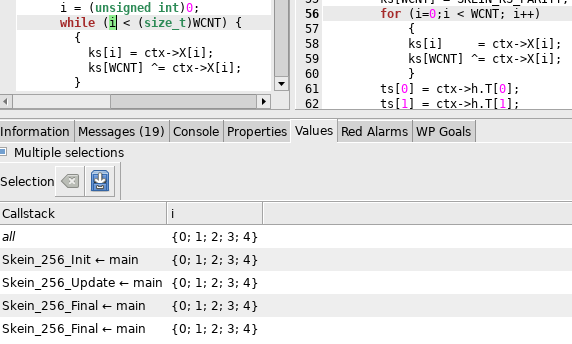
\includegraphics[width=0.75\textwidth]{gui-images/gui-loop-to-unroll.png}
\caption{Estimating loop unroll bounds in the GUI}
\label{fig:gui-loop-to-unroll}
\end{figure}

In this case, \verb|WCNT| has a constant value (4), so it could also be used
to estimate the loop bounds.

We can then Ctrl+click on the loop condition in the original source view
(right panel) to open an editor\footnote{The external code editor used by the GUI
  can be defined via the menu {\em File - Preferences}.} centered on the loop, and
then add the loop unroll annotation, as follows:

\begin{listing-nonumber}
  //@ loop unroll 4;
  for (i=0;i < WCNT; i++)
      {
      ks[i]     = ctx->X[i];
      ks[WCNT] ^= ctx->X[i];            /* compute overall parity */
      }
\end{listing-nonumber}

The value 4 is sufficient to completely unroll the loop, even though \verb|i|
ranges from 0 to 4 (5 values in total). One way to confirm the unrolling is
complete is to check that ``starting to merge loop iterations'' is no
longer emitted when entering the loop. Also, when a loop unroll annotation
is present but insufficient to unroll the loop, a message is emitted:

\begin{logs}
[eva:loop-unroll] skein_block.c:57: loop not completely unrolled
\end{logs}

Once a loop is completely unrolled, any ``leftovers'' are ignored, so it incurs
no extra cost. Using a value larger than necessary is therefore not an issue.

The practical effect of adding this annotation and then re-running \Eva{} is
the elimination of 3 alarms in the analysis. Thanks to the extra precision
allowed by the annotation (with a minimal increase in analysis time), \Eva{}
is now able to prove there are no initialization errors in more places than
before.

\subsection{Increasing precision}

Option \verb|-eva-precision| allows setting a global trade-off between
precision and analysis time. By default, \Eva{} is tuned to a low precision
to ensure a fast initial analysis. Especially for smaller code bases, it is
often useful to increase this precision, to dismiss ``easy'' alarms.
Precision can be set between 0 and 11, the higher the value, the more precise
the analysis. The default value of \Eva{} is somewhere between 0 and 1, so that
setting \verb|-eva-precision 0| potentially allows it to go even faster
(only useful for large or very complex code bases).

\verb|-eva-precision| is in fact a meta-option, whose only purpose is to set
the values of other options to a set of predefined values. This avoids the user
having to know all of them, and which values are reasonable. Think of it as a
``knob'' to perform a coarse adjustment of the analysis, before fine-tuning
it more precisely with other options.

\verb|-eva-precision| displays a message when it is used, stating which options
are affected and the value given to them. If one of those options is already
specified by the user, that value takes priority over the one chosen by
\verb|-eva-precision|.

Among the options set by \verb|-eva-precision|, there is \verb|-eva-slevel|,
which can be thought of as some kind of ``fuel''
to be consumed during the analysis: as long as there is some slevel,
the analysis will keep states separated and maintain precision at the cost of
extra analysis time; when all of
it is consumed, further states are merged, avoiding increase in analysis time
but approximating the results. It can also be
specified separately for each function (\verb|-eva-slevel-function f:n|).

For complex code bases, however, \verb|-eva-slevel| lacks in stability and
predictability: it is very hard to determine exactly {\em how} it is used.
It can be consumed in the presence of loops, branches, disjunctions;
in nested loops, it is consumed by both inner and outer loops.
In loops with branches, its consumption may become exponential.
And once a satisfactory value is found, later changes to the source code,
ACSL specifications, \Eva{}'s algorithms or other parameters can affect it,
requiring a new parametrization.

In our example, we can quickly try a few values of \verb|-eva-precision|,
such as 1, 2 and 3:

\begin{frama-c-commands}
frama-c -eva-precision 3 -eva *.c > log
\end{frama-c-commands}

Now, the analysis goes rather far without finding any alarm,
but when it is almost done (after the analysis of function
\lstinline|Skein_256_Final|), it produces:
\begin{logs}
...
[eva] using specification for function printf_va_1
[eva:alarm] main_1.c:17: Warning:
  accessing uninitialized left-value. assert \initialized(&hash[i]);
[eva] Done for function main
...
\end{logs}

There remains an alarm about initialization, but all the others have been
removed. Trying larger values for precision or slevel does not change this.
In this case, we can afford to spend some time looking at it in more detail.

\subsection{Inspecting alarms in the GUI}

Instead of running \verb|frama-c|, let us use \verb|frama-c-gui|:

\begin{frama-c-commands}
frama-c-gui -eva-precision 3 -eva *.c > log
\end{frama-c-commands}

The GUI allows the user to navigate the source code, to inspect the sets of
values inferred by the analysis and to get
a feeling of how it works. Right-clicking on the function name
at a call site brings a contextual menu to jump
to the function's definition.
In order to return to the caller,
right-clicking on the name of the current function at the top
brings a contextual menu with a list of callers.
You can also use the Back button (left arrow) in the toolbar.
The Information panel also offers navigation possibilities between
variables and their definitions.

In the graphical interface, three panels (displayed below the
source code) are very useful for \Eva{}: Properties, Values, and
Red Alarms. Further details about the GUI are presented in chapter~\ref{gui}.
For now, it suffices to say that:

\begin{itemize}
\item Properties displays (among others) the list of alarms in the program;
\item Values displays the inferred values for the expression selected in the
  Frama-C normalized source code (highlighted in green);
\item Red Alarms displays some special cases of alarms that should be considered
  first.
\end{itemize}

In the GUI, each alarm is represented with a ``bullet'' to its left.
Red bullets mean ``this {\em always} happens''; yellow
bullets mean ``this {\em may} happen (but I am not sure, due to
approximations)''. When there are several alarms, some strategies allow
prioritizing which alarms are more likely to correspond to actual issues.

The overall rule of thumb when inspecting alarms in the GUI\footnote{The first
  time the Frama-C GUI is run, the Properties panel displays several kinds of
  properties. For \Eva{}, the most useful view consists in selecting the
  ``Reset 'Status' filters to show only unproved/invalid'' option, using the
  button next to ``Refresh'' in the Properties panel.} is the following:

\begin{itemize}
\item inspect red alarms in the Properties panel; these correspond to
  situations where the analysis is {\em certain} that a problem has arrived;
  either an actual bug in the code, or some issue in the analysis that needs to
  be addressed (e.g. due to missing or incorrect specifications);
\item inspect the cases present in the Red Alarms panel; these are situations
  which are likely to correspond to definitive problems, and thus should be
  treated before others\footnote{The {\em exact} meaning of such red alarms is
    too complex to be presented here; as a first approximation, these can be
    seen as intermediate between red and yellow alarms.};
\item inspect remaining cases (yellow alarms) in the Properties panel.
\end{itemize}

In the case of our remaining alarm, it is yellow, but it appears in the
Red Alarms panel. This indicates it is more likely to correspond to a real
issue.

Extra information can be observed by clicking the alarm in the Red Alarms tab,
which highlights it in the source code, then selecting expression
\lstinline|hash| in line 17 and reading the \textsf{Values} tab:
\begin{logs}
  [0] $\in$ {200}
  [1..7] $\in$ UNINITIALIZED
\end{logs}
This means that element \lstinline|hash[0]| has value 200, but elements 1 to 7
are definitely uninitialized. Therefore the first iteration of the loop
proceeds as expected, but on the second iteration, the analysis of the branch
is stopped, because
from the point of view of the analyzer, reading an uninitialized
value should be a fatal error. And there are no other execution
branches that reach the end of this loop, which is why the analyzer
finds that function \lstinline|main| does not terminate (the log contains
the message ``NON TERMINATING FUNCTION'').

\subsection{Finding and fixing bugs}

We found a real issue in the code, but to find the exact cause it is necessary
to investigate the code.
Looking again at the header file \lstinline|skein.h|, we may now
notice that in function \lstinline|Skein_256_Init|,
the formal parameter for the desired hash length is named
\lstinline|hashBitLen|. This parameter should certainly be expressed in bits!
We were inadvertently asking for a 1-char hash of the message
since the beginning, and the test that we ran as our first
step failed to notice it.

The bug can be fixed by passing
8*HASHLEN instead of HASHLEN as the second argument of
\lstinline|Skein_256_Init|.
With this fix in place, the analysis
with \lstinline|-eva-precision 3| produces no alarms and gives the following
result:
\begin{logs}
Values for function main:
  hash[0] $\in$ {40}
      [1] $\in$ {234}
      [2] $\in$ {138}
      [3] $\in$ {230}
      [4] $\in$ {134}
      [5] $\in$ {120}
      [6] $\in$ {37}
      [7] $\in$ {35}
  i $\in$ {8}
\end{logs}

Meanwhile, compiling and executing the fixed test produces the result:
\begin{logs}
40
234
138
230
134
120
37
35
\end{logs}

\section{Guaranteeing the absence of bugs}

\subsection{Generalizing the analysis to arbitrary messages of fixed length}

The analysis we have done so far is very satisfying because
it finds problems that are not detected by a C compiler or by testing.
The results of this analysis only prove
the absence of run-time errors\footnote{and the absence
of conditions that
{\em should} be run-time errors -- like the uninitialized access already
encountered} when the particular message that we
chose is being hashed, though.
It would be much more useful to have the assurance that there are
no run-time errors for any input message, especially since the library
might be under consideration for embedding in a device where anyone
(possibly a malicious user) will be able to choose the message
to hash.

A first generalization of the previous analysis  is to include
in the subject matter
the hashing of all possible 80-character messages. We can do this
by separating the analyzed program in two distinct phases, the first
one being the construction of a generalized analysis context
and the second one being made of the sequence of function calls
that we wish to study:

\listinginputcaption{1}{\texttt{main\_2.c}}{tutorial/main_2.c}

From this point onward the program is no longer executable because
of the call to builtin primitives such as \lstinline|Frama_C_interval|.
We therefore dispense with the final calls to \lstinline|printf|,
since \Eva{} offers simpler ways to observe intermediate
and final results. Note that we included \verb|__fc_builtin.h|, a file
that comes from the Frama-C distribution and which
defines \lstinline|Frama_C_interval|. Running Frama-C on this
file (without \verb|main_1.c| in the same directory, to avoid having two
definitions for \verb|main|):
\begin{frama-c-commands}
frama-c -eva-precision 3 -eva *.c > log 2>&1
\end{frama-c-commands}

This time, the absence of actual alarms is starting to be really interesting:
it means that it is formally excluded that the functions
\lstinline|Skein_256_Init|, \lstinline|Skein_256_Update|, and
\lstinline|Skein_256_Final| produce a run-time error when
they are used, in this order, to initialize a local variable
of type \lstinline|Skein_256_Ctxt_t| (with argument 64 for the size),
parse an arbitrary message and produce a hash in a local \lstinline|u08b_t|
array of size~8.

\subsection{Verifying functional dependencies}

If we had written a formal specification for function Skein, we would soon
have expressed that we expected it to modify the buffer \lstinline|hash|
that is passed to \lstinline|Skein_256_Final| (all 8 bytes of the buffer),
to compute the new contents of this buffer from the contents of the
input buffer \lstinline|msg| (all 80 bytes of it), and from nothing else.

During \Eva{}'s analysis, we have seen that all of the buffer \verb|hash|
was always modified in the conditions of the analysis: the reason is that
this buffer was uninitialized before the sequence of calls,
and guaranteed to be initialized after them.

We can get the complete list of locations that may be modified by each
function by adding the option \verb|-out| to the other options we were
already using. These locations are computed in a quick analysis that comes
after \Eva{}. In the results of this analysis, we find:
\begin{logs}
[inout] Out (internal) for function main:
          Frama_C_entropy_source; msg[0..79]; i; hash[0..7]; skein_context; tmp
\end{logs}
The ``(internal)'' reminds us that this list includes the local variables
of \lstinline|main| that have been modified. Indeed, all the variables
that we could expect to appear in the list are here: the input buffer, that
we initialized to all possible arbitrary 80-char messages; the loop index
that we used in doing so; the output buffer for receiving the hash;
and Skein's internal state, that was indirectly modified by us when we called
the functions \lstinline|Init|, \lstinline|Update| and \lstinline|Final|.

If we want the outputs of the sequence to appear more clearly, without the
variables we used for instrumenting, we can put it in its own function:

\begin{listing}{1}
u08b_t hash[HASHLEN];

void do_Skein_256(void)
{
  Skein_256_Ctxt_t skein_context;
  Skein_256_Init( &skein_context, HASHLEN * 8);
  Skein_256_Update( &skein_context, msg, 80);
  Skein_256_Final( &skein_context, hash);
}

void main(void)
{
  int i;

  for (i=0; i<80; i++) msg[i]=Frama_C_interval(0, 255);

  do_Skein_256();
}
\end{listing}

Using option \verb|-out-external| in order to obtain lists of
locations that exclude each function's local variables, we get:
\begin{logs}
[inout] Out (external) for function do_Skein_256:
          hash[0..7]
\end{logs}
This means that no location other than \lstinline|hash[0..7]| was
modified by the sequence of calls to Skein-256 functions. It doesn't
mean that each of the cells of the array was overwritten: we have to
rely on the results of \Eva{} when \lstinline|hash| was a
local variable for that result. But it means that when used in
conformance with the pattern in this program, the functions do not
accidentally modify a global variable. We can conclude from this
analysis that the functions are re-entrant as long as the concurrent
computations are being made with separate contexts and destination
buffers.

Keeping the convenient function \lstinline|do_Skein_256| for modeling the
sequence, let us now compute the functional dependencies of each function.
Functional dependencies list, for each output location,
the input locations that influence the final contents of this output location:
\begin{frama-c-commands}
frama-c -eva *.c -eva-precision 3 -deps
\end{frama-c-commands}
\begin{logs}
Function Skein_256_Init:
  skein_context.h.hashBitLen FROM ctx; hashBitLen
               .h{.bCnt; .T[0..1]; } FROM ctx
               .X[0..3] FROM msg[0..63];
                             skein_context{.X[0..3]; .b[0..31]; }; ctx;
                             hashBitLen; Skein_Swap64_ONE[bits 0 to 7] (and SELF)
               .b[0..31] FROM ctx (and SELF)
  \result FROM \nothing

Function Skein_256_Update:
  skein_context.h.bCnt FROM skein_context.h.bCnt; ctx; msgByteCnt
               .h.T[0] FROM skein_context.h{.bCnt; .T[0]; }; ctx; msgByteCnt
               .h.T[1] FROM skein_context{.h.bCnt; .h.T[1]; }; ctx;
                            msgByteCnt
               {.X[0..3]; .b[0..15]; } FROM msg[0..79];
                                            skein_context{.h{.bCnt; .T[0..1]; };
                                                          .X[0..3]; .b[0..31]; };
                                             ctx; msg_0; msgByteCnt (and SELF)
  \result FROM \nothing

Function Skein_256_Final:
  hash[0..7] FROM msg[0..79]; skein_context; ctx;
                  hashVal; Skein_Swap64_ONE[bits 0 to 7] (and SELF)
  skein_context.h.bCnt FROM skein_context.h.hashBitLen; ctx (and SELF)
               .h.T[0] FROM skein_context.h{.hashBitLen; .bCnt; .T[0]; }; ctx
               .h.T[1] FROM skein_context{.h.hashBitLen; .h.T[1]; }; ctx
               {.X[0..3]; .b[0..15]; } FROM msg[0..79]; skein_context; ctx;
                                            Skein_Swap64_ONE[bits 0 to 7]
                                            (and SELF)
               .b[16..31] FROM skein_context.h.bCnt; ctx (and SELF)
  \result FROM \nothing
\end{logs}
The functional dependencies for the functions \lstinline|Init|,
\lstinline|Update| and \lstinline|Final| are quite cryptic. They refer
to fields of the struct \lstinline|skein_context|. We have not had
to look at this struct yet, but its type \lstinline|Skein_256_Ctxt_t|
is declared in file \verb|skein.h|.

In the results, the mention \verb|(and SELF)| means that parts of the output
location may keep their previous values. Conversely, absence of this
mention means that the output location is guaranteed to have been completely
over-written when the function returns.
For instance, the field \lstinline|skein_context.h.T[0]| is
guaranteed to be over-written with a value that depends only on
various other subfields of \lstinline|skein_context.h|. On the other
hand, the \verb|-deps| analysis does not guarantee that all cells of
\verb|hash| are over-written --- but we previously saw we
could deduce this information from \Eva{}'s results.

Since we don't know how the functions are supposed to work,
it is difficult to tell if these
dependencies are normal or reveal a problem. Let us move on to the
functional dependencies of \lstinline|do_Skein_256|:
\begin{logs}
Function do_Skein_256:
  hash[0..7] FROM msg[0..79]; Skein_Swap64_ONE[bits 0 to 7] (and SELF)
\end{logs}

These dependencies make the effect of the functions clearer.  The
\verb|FROM msg[0..79]| part is what we expect.  The
\verb|and SELF| mention is an unfortunate approximation.  The
dependency on global variable \verb|Skein_Swap64_ONE| reveals an implementation
detail of the library (the variable is used to detect endianness
dynamically). Finding out about this variable is a good thing: it
shows that a possibility for a malicious programmer to corrupt the
implementation into hashing the same message to different digests
would be to try to change the value of \verb|Skein_Swap64_ONE| between
computations.  Checking the source code for mentions of variable
\lstinline|Skein_Swap64_ONE|, we can see it is used to
detect endianness and is declared \lstinline|const|. On an
MMU-equipped platform, there is little risk that this variable
could be modified maliciously from the outside.
However, this is a vivid example of how static
analysis, and especially correct analyses as provided in Frama-C, can
complement code reviews in improving trust in existing C code.

Assuming that variable \lstinline|Skein_Swap64_ONE| keeps its value, a same
input message is guaranteed always to be hashed by this
sequence of calls to the same digest,
because option \verb|-deps| says that there is no other
memory location \lstinline|hash| is computed from, not even an
internal state.

A stronger property to verify would be that the
sequence \lstinline|Init(...)|, \lstinline|Update(...,80)|,
\lstinline|Final(...)| computes the same hash as when the
same message is passed in two calls \lstinline|Update(...,40)|.
This property is beyond the reach of \Eva{}.
In the advanced tutorial, we show how to verify easier properties
for sequences of calls that include several calls
to \lstinline|Update|.

\subsection{Generalizing to arbitrary numbers of Update calls}

As an exercise, try to verify that there cannot be a run-time error
when hashing arbitrary contents by
calling \lstinline|Update(...,80)| an arbitrary number of times
between \lstinline|Init| and \lstinline|Final|.  The general strategy
is to modify the C analysis context we have already written in a way
such that it is evident that it captures all such sequences of calls,
and also in a way that launched with adequate options,
\Eva{} does not emit any warning.

The latter condition is harder than the former.
Observing results (with the GUI or observation functions
described in section \ref{buitins_observation}) can help to iterate towards
a solution. Be creative. The continuation of this tutorial can be found online
at \url{https://frama-c.com/category/skein/}\footnote{Note that some
  messages and options have changed since the tutorial was posted. Using an
  older Frama-C version may be necessary to obtain similar results.}
; read available posts in chronological order.

% This tutorial is TO BE CONTINUED.\\
% ~\\
% In the next episode, you will learn how to
% verify the hashing of messages of all lengths, and how to use
% other Frama-C analyses to
% establish more interesting results about Skein-256.
% One of the strong properties that we will verify is that
% it is {\em platform-conforming}\footnote{The notion here is almost the same as
% that of {\em strictly conforming program} in the ``Conformance'' chapter of the
% C99 standard, but \Eva{} recognizes some widely-used constructs
% that are not specified in the standard, as discussed in \ref{norme_pratique}}: for
% a given platform configuration,
% two sequences of calls to the Skein-256 functions, part of the same
% or of different programs, always compute the same hash for the same message.

% If this seems unimpressive, then please consider the attacker's
% point of view.
% Assume for an instant that it is important for you to be able
% to make the Skein-256 functions, inserted in different contexts, compute
% different hashes for a message of your choice.
% Think of all the ways you would have, in C,
% as a malicious  developer of the library, to insert backdoors in
% its source code to make it fail this property.
% In the next episode, you will discover how your
% best try would have been to surreptitiously change the value of variable
% ONE. But as long as this variable is kept to its normal value
% (and being declared \lstinline|static const|, you can even trust the
% compiler to enforce that, although it would be better to analyze
% the rest of the program to be on the safe side), no calling context can
% make the Skein functions compute different hashes for one same message.



\chapter{What \Eva{} provides}\label{what}
\vspace{2cm}

{\em Here begins the reference section of this manual.\\
This chapter categorizes and describes the outputs of \Eva{}.}

\vspace{2cm}

\section{Values}
\label{sec:values}

The \Eva{} plug-in accepts queries for the value of
a variable \lstinline|x| at a given program point. It answers such a
query with an over-approximation of the set of values possibly taken
by \lstinline|x| at the designated point for all possible executions.


\subsection{Variation domains for expressions}\label{valeurs}
%%%%%%%%%%%%%%% A DECRIRE :

% S3.i1[bits 0 to 7]# -> {4369} misaligned 0%16

The variation domain of a variable or expression can take one of
the shapes described below.

\subsubsection{A set of integers}
The analyzer may have determined the variation domain of a variable is
a set of integers.  This usually happens for variables of an integer
type, but may happen for other variables if the application contains
unions or casts. A set of integers can be represented as:

\begin{itemize}
\item an enumeration, $\cbopen v_1;\ \ldots\ v_n\cbclose$,
\item an interval, $\bropen l{\tt ..}u\brclose$, that represents all
  the integers comprised between $l$ and $u$. If ``\lstinline|--|'' appears
  as the lower bound $l$ (resp. the upper bound $u$), it means that the
  lower bound (resp upper bound) is $-\infty$ (resp. $+\infty$),
\item an interval with periodicity information,
  $\bropen l..u\brclose\mbox{\tt\/,}r\mbox{\tt \%}m$,
  that represents the set of values comprised between $l$ and $u$
  whose remainder in the Euclidean division by $m$ is equal to $r$.
  For instance, $\bropen 2..42\brclose\mbox{\tt\/,}2\mbox{\tt \%}10$,
  represents the set that contains 2, 12, 22, 32, and 42.
\end{itemize}

\subsubsection{A floating-point value or interval}
A location in memory (typically a floating-point variable)
may also contain a floating-point number
or an interval of floating-point numbers:
  \begin{itemize}
  \item $f$ for the non-zero floating-point number $f$ (the floating-point number \lstinline|+0.0| has the same representation as the integer \lstinline|0| and is identified with it),
  \item $\bropen f_l\ ..\ f_u\brclose$ for the interval from $f_l$ to
$f_u$ inclusive.
  \end{itemize}
\subsubsection{A set of addresses}
A variation domain (for instance for a pointer variable)
may be a set of addresses, denoted by
       $\cbopen\cbopen a_1;\ \ldots\ a_n \cbclose\cbclose$.
Each $a_i$ is of the form:
  \begin{itemize}
  \item $\&x + D$, where $\&x$ is the base address corresponding to the
    variable $x$, and $D$ is in the domain of integer values and represents
    the possible offsets {\bf expressed in bytes} with respect to the base
    address $\&x$. When $x$ is an array or an aggregate, and $D$ corresponds
    to the offset(s) of a field or an array cell, a concrete C-like syntax
    may be used, i.e. \verb+&t{[1].i1, [2].i2}+.
  \item $\mbox{\tt NULL} + D$, which denotes absolute addresses (seen
as offsets with respect to the base address NULL).
  \item $\mbox{\tt "foo"} + D$, which denotes offsets from a literal
string with contents ``foo''.
  \end{itemize}
In all three cases, ``${}+D$'' is omitted if $D$ is $\{0\}$, that is,
when there is no offset.

\subsubsection{An imprecise mix of addresses}
If the application involves, or seems to involve, unusual arithmetic
operations over addresses, many of the variation domains provided by
the analysis may be imprecise sets of the form
 $\mbox{\tt garbled mix of }\&\cbopen x_1;\ \ldots\ x_n \cbclose$.
This expression
 denotes an unknown value built from applying arithmetic operations
to the addresses of variables $x_1$,\ldots,$x_n$ and to integers.

\subsubsection{Absolutely anything}
You should not observe it in practice, but sometimes the analyzer is
not able to deduce any information at all on the value of a variable,
in which case it displays $\mbox{\tt ANYTHING}$ for the variation
domain of this variable.

\subsection{Memory contents}

Memory locations can contain, in addition to the above sets of values,
uninitialized data and dangling pointers. It is illegal to use these
special values in computations, which is why they are not listed as
possible values for an expression. Reading from a variable that
appears to be uninitialized causes an alarm to be emitted, and
then the set of values for the variable is made of those initialized
values that were found at the memory location.

\subsection{Interpreting the variation domains}

Most modern C compilation platforms unify integer values
and absolute addresses:
there is no difference between the encoding of the integer 256
and that of the address \lstinline|(char*)0x00000100|. Therefore, \Eva{}
does not distinguish between these two values either. It is partly
for this reason that offsets $D$ are expressed
in bytes in domains of the form $\cbopen\cbopen \&x + D;\ \ldots\ \cbclose\cbclose$.

\subsubsection{Examples of variation domains}

\begin{itemize}

\item \lstinline|{3, 8, 11}| represents exactly the integers 3, 8 and 11.

\item \lstinline|[1..256]| represents the set of integers comprised between 1 and 256, each of which can also be interpreted as an absolute address between
0x1 and 0x100.

\item \lstinline|[0..256],0%2|
      represents the set of even integers comprised between 0 and 256.
This set is also the set of the addresses of the first 129 aligned 16-bit words
in memory.

\item \lstinline|[1..255],1%2|
      represents the odd integers comprised between 1 and 255.

\item \lstinline|[--..--]| represents the set of all (possibly negative)
integers that fit within the type of the variable or expression that is
being printed.

\item \lstinline|{3.}| represents the floating-point number \lstinline|3.0|.

\item \lstinline|[-3. .. 9.]| represents the interval of floating-point values
comprised between \lstinline|-3.0| and \lstinline|9.0|.

\item \lstinline|[-3. .. 9.] $\cup$ {NaN}| represents the same
  interval as above, plus \lstinline|NaN|.

\item \lstinline|[-inf .. 3.4]| represents the interval of
  floating-point values comprised between $-\infty$ and \lstinline|3.4|.

\item \lstinline|[-inf .. inf] $\cup$ {NaN}| represents
  all possible floating-point values.

\item \lstinline|{{ &x }}| represents the address of the variable \lstinline|x|.

\item \lstinline|{{ &x + { 0; 1 } }}|
  represents the address of one of the first two bytes of variable
      \lstinline|x| -- assuming \lstinline|x| is of a type at least 2 bytes in size.
 Otherwise, this notation represents a set containing the address of
\lstinline|x| and an invalid address.

\item \lstinline|{{ &x ; &y }}|
      represents the addresses of \lstinline|x| and \lstinline|y|.

\item \lstinline|{{ &t + [0..256],0%4 }}|, in an application where
  \lstinline|t| is declared as an array of 32-bit integers, represents
  the addresses of locations \lstinline|t[0]|, \lstinline|t[1]|, \ldots, \lstinline|t[64]|.

\item \lstinline|{{ &t + [0..256] }}|
represents the same values as the expression \lstinline|(char*)t+i|
where the variable \lstinline|i| has an integer value comprised between 0 and 256.

\item \lstinline|{{ &t + [--..--] }}|
      represents all the addresses obtained by shifting \lstinline|t|, including
some misaligned and invalid ones.

\end{itemize}

\subsection{Origins of approximations}

Approximated values may  contain
information about the origin of the approximations.  In this
case the value is shown as ``\lstinline|$\mbox{\tt garbled mix of }\&\cbopen x_1;\ \ldots\ x_n \cbclose$ (origin: ...)|''.
The text provided after ``\lstinline|origin:|'' indicates the
location and the cause of
some of these approximations.
\goodbreak

Most origins are of the form \lstinline|Cause L|, where \lstinline|L|
is an (optional) line or the application indicating where the approximation
took place. Origin causes are one of the following:

\subsubsection{Arithmetic operation}
The origin \lstinline$Arithmetic L$ denotes arithmetic operations over
addresses, whose result cannot be precisely represented by the analyzer.
\csource{examples/ari.c}
In this example, the return value for \lstinline|f| is:

\begin{logs}
{{ garbled mix of &{x; y} (origin: Arithmetic {ari.c:4}) }}
\end{logs}

\subsubsection{Misaligned read}

The origin \lstinline$Misaligned read L$ indicates that
misaligned reads prevented the computation to be precise.
A misaligned read is a memory read-access where the bits read were not
previously written as a single write that modified the whole set of
bits exactly.

An example of a program leading to a misaligned read is the following:
\csource{examples/misa.c}
The value returned by the function \lstinline|main| is\\
\lstinline|{{ garbled mix of &{x; y} (origin: Misaligned read {misa.c:6}) }}|.\\
The analyzer is by default configured for a 64-bit architecture,
and that consequently the read memory access is not an out-of-bound access.
If it was, an alarm would be emitted, and the
analysis would go in a different direction.

With the default target platform, the read access remains
within the bounds of array \lstinline|t|,
but due to the offset of six bytes,
the 32-bit word read is made of the last two bytes from \lstinline|t[0]|
and the first two bytes from \lstinline|t[1]|.

\subsubsection{Misaligned writes}

The origin \lstinline$Misaligned write L$ indicates that the interpretation of
a misaligned write to an imprecise location has created a garbled mix at this
memory location.

An example of a program where a misaligned write creates a garbled mix
is the following:
\csource{examples/misa_write.c}

The interpretation of the last assignment by the analysis writes
the imprecise value
\lstinline|{{ garbled mix of &{x} (origin: Misaligned write {misa.c:6}) }}|
into the array \lstinline|t|.

\subsubsection{Call to an unknown function}
The origin \lstinline$Library function L$ arises from the interpretation
of a function specification, when an \lstinline|assigns| clause applies to
pointer values.
A function specification is only used for:
\begin{itemize}
\item
  functions whose body is not provided, and for which no Eva builtins
  exist. See section~\ref{builtins-list} for a list of available builtins.
\item
  recursive functions that cannot be completely analyzed;
  see section~\ref{recursion} for more details.
\item
  functions given to the \verb+-eva-use-spec+ option;
  see section~\ref{val-use-spec} for more details.
\end{itemize}

\subsubsection{Fusion of values with different alignments}
The notation \lstinline$Merge L$ indicates that memory states with incompatible
alignments are fused together. In the example below,
the memory states from
the then branch and from the else branch contain in the array
\lstinline|t| some 32-bit addresses with incompatible alignments.
\csource{examples/merge.c}
The value returned by function \lstinline|main| is:

\begin{logs}
{{ garbled mix of &{ x; y } (origin: Merge { merge.c:10 }) }}
\end{logs}

\subsubsection{Well value}

When generating an initial state to start the analysis from
(see section \ref{libentry} for details), the analyzer
has to generate a set of
possible values for a variable with only its type for information.
Some recursive or deeply chained types may force the generated
contents for the variable to contain imprecise, absorbing values
called well values.

Computations that are imprecise because of a well value are marked
as \lstinline|origin: Well|.

\section{What is checked by \Eva{}}\label{obligations}

\Eva{} warns about possible run-time errors in the analyzed
program, through the means of \emph{proof obligations}: the errors that cannot
be proved by the \Eva{} plug-in are left to be proved by other plug-ins.
%% The correctness of the results provided by \Eva{}
%% is guaranteed only if the user verifies all the
%% proof obligations generated during the analysis.
These proof obligations
are displayed as messages that contain the word \lstinline|assert| in
the textual log. Within Frama-C's AST, they are also available ACSL predicates.
(Frama-C comes with a common specification language for all plug-ins,
called ACSL, described at \url{http://frama-c.com/acsl.html}.)

When using the GUI version of Frama-C, proof obligations are
inserted in the normalized source code. With the batch version,
option \lstinline|-print| produces a version of the analyzed source code
annotated with the proofs obligations.  The companion option
\lstinline|-ocode <file.c>| allows to specify a filename for the
annotated source code to be written to.

\subsubsection{Invalid memory accesses}
Whenever \Eva{} is not able to establish that
a dereferenced pointer is valid, it emits an alarm that expresses
that the pointer needs to be valid at that point. Likewise, direct
array accesses that may be invalid are flagged.

\csource{examples/alarms/invalid.c}
In the above example, the analysis is not able to guarantee that
the memory accesses \lstinline|t[i]| and \lstinline|*p| are valid,
so it emits a proof obligation for each:
\begin{logs}
invalid.c:5: ... accessing out of bounds index. assert i < 10;
invalid.c:7: ... out of bounds write. assert \valid(p);
\end{logs}
(Notice that no alarm \lstinline|assert 0 <= i| is emitted, as the
analysis is able to guarantee that this always holds.)


The choice between these two kinds of alarms is influenced by
option \lstinline|-unsafe-arrays|, as described
page \pageref{unsafe-arrays}.

Note that line 6 or 8 in this example could be considered as
problematic in the strictest interpretation of the standard.
\Eva{} omits warnings for these two lines according
to the attitude described in \ref{norme_pratique}. An option
to warn about these lines could happen if there was demand for
this feature.

\subsubsection{Invalid pointer arithmetic}

By default, \Eva{} does \emph{not} emit alarms on invalid pointer arithmetic:
alarms are only emitted when an invalid pointer is dereferenced or wrongly used
in a comparison, not at the creation of such pointers.

However, if the \lstinline|-warn-invalid-pointer| option is enabled,
\Eva{} emits an alarm when an operation may create a pointer that does
not point inside an object or one past an object,
even if this pointer is not used afterward.

This may happen on:
\begin{itemize}
\item addition (or subtraction) of an integer from a pointer, when the analysis
  is unable to prove that the resulting pointer points inside, or one past,
  the same object pointed to by the initial pointer.
  In this case, the emitted alarm reports a possible undefined behavior.
\item conversion of an integer into a pointer. Except for the constant~0,
  such a conversion is always an implementation-defined behavior
  according to the \isoc{} standard. However, a footnote also explains that
  conversion between pointers and integers is ``\emph{intended to
  be consistent with the addressing structure of the execution environment}''.
  This is why Eva also authorizes conversion of integers:
  \begin{itemize}
  \item in the range of valid absolute addresses
    (according to \texttt{absolute-valid-range})
  \item computed from the address of an object \lstinline|o| such that the
    resulting pointer points inside or one past the object \lstinline|o|.
  \end{itemize}
  In all other cases, an alarm is emitted, which reports the possible
  implementation-defined behavior mentioned above.
\end{itemize}

In the example below, the first increment of the pointer \lstinline|p| is valid,
although the resulting pointer should not be dereferenced. The second increment
leads to an invalid alarm when option \lstinline|-warn-invalid-pointer| is on.
\csource{examples/alarms/pointer_arith.c}
\begin{logs}
  [eva:alarm] pointer_arith.c:4: Warning:
    invalid pointer creation. assert \object_pointer(p + 1);
\end{logs}

In the same way, in the example below, the first conversion at line~5
does not generate an alarm, but the second conversion leads to an invalid alarm
with option \lstinline|-warn-invalid-pointer|.

\csource{examples/alarms/pointer_conversion.c}
\begin{logs}
  [eva:alarm] pointer_arith.c:6: Warning:
    invalid pointer creation. assert \object_pointer((char *)(a + 2));
\end{logs}


\subsubsection{Division by zero}
When dividing by an expression that the analysis
is not able to guarantee non-null, a proof
obligation is emitted. This obligation expresses that the divisor
is different from zero at this point of the code.

In the particular case where zero is the only possible value
for the divisor, the analysis stops the propagation of this
execution path.
If the divisor seems to be able to take non-null values,
the analyzer
is allowed to take into account the
property that the divisor is different from zero when it continues
the analysis after this point.
The property expressed by an alarm may also not be taken into account
when it is not easy to do so.
\csource{examples/alarms/div.c}
\begin{logs}
div.c:4: ... division by zero. assert (int)(x*y) $\not\equiv$ 0;
div.c:5: ... division by zero. assert x $\not\equiv$ 0;
\end{logs}
In the above example, there is no way for the analyzer
to guarantee that \lstinline|x*y| is not null, so it emits
an alarm at line 4. In theory, it could avoid emitting
the alarm \lstinline|x $\not\equiv$ 0| at line 5
because this property is a consequence of the property emitted
as an alarm at line 4. Redundant alarms happen -- even in cases
simpler than this one. Do not be surprised by them.

\subsubsection{Undefined logical shift}
Another arithmetic alarm is the alarm emitted for logical
shift operations on integers where the second operand may be
larger than the size in bits of the first operand's type.
Such an operation is left undefined by the \isoc{} standard, and
indeed, processors are often built in a way that such an
operation does not produce the \lstinline|0| or \lstinline|-1|
result that could have been expected. Here is an example
of program with such an issue, and the resulting alarm:
\csource{examples/alarms/shift.c}
\begin{logs}
shift.c:4: ... invalid RHS operand for shift. assert 0 $\le$ c < 32;
\end{logs}

\Eva{} also detects shifts on negative integers.
Left-shifting a negative integer is an undefined behavior according to the
\isoc{} standard, and leads to an alarm by default.
These alarms can be disabled by using the option
\lstinline|-no-warn-left-shift-negative|.
Right-shifting a negative integer is an implementation-defined operation,
and does not lead to an alarm by default.
However, the option \lstinline|-warn-right-shift-negative| can be used to
enable such alarms.

\csource{examples/alarms/lshift.c}
\begin{logs}
[eva:alarm] lshift.c:4: Warning:
  invalid LHS operand for left shift. assert 0 $\le$ x;
\end{logs}

\subsubsection{Overflow in integer arithmetic}

By default, \Eva{} emits alarms for --- and reduces the
sets of possible results of --- signed arithmetic computations where
the possibility of an overflow exists. Indeed,
such overflows have an undefined behavior according to
paragraph 6.5.5 of the \isoc{} standard.
%
If useful, it is also possible to assume that signed integers overflow
according to a 2's complement representation. The option
\lstinline|-no-warn-signed-overflow| can be used to this end. A
reminder warning is nevertheless emitted on operations that are detected
as potentially overflowing. This warning can also be disabled by option
\lstinline|-eva-warn-key signed-overflow=inactive|.

By default, no alarm is emitted for arithmetic operations on unsigned integers
for which an overflow may happen, since such operations have
defined semantics according to the \isoc{} standard.
If one wishes to signal and prevent such unsigned overflows,
option \verb+-warn-unsigned-overflow+ can be used.

By default, Eva emits alarms for downcasts of pointer values to (signed
or unsigned) integer types. Such downcasts are indeed  undefined behavior
according to section 6.3.2.3, §6 of the \isoc{} standard.
However, option \lstinline|-no-warn-pointer-downcast| can be used to disable
these alarms.

Finally, by default, no alarm is emitted for downcasts to signed or unsigned
integers. In the signed case, the least significant bits
of the original value are used, and are interpreted according
to 2's complement representation.
Frama-C's options \lstinline|-warn-signed-downcast| and
\lstinline|-warn-unsigned-downcast| can be used to emit alarms on signed
or unsigned downcasts that may exceed the destination range.


\subsubsection{Overflow in conversion from floating-point to integer}
An alarm is emitted when a floating-point value appears to exceed the
range of the integer type it is converted to.

\csource{examples/alarms/ov_float_int.c}
\begin{logs}
...
[eva:alarm] ov_float_int.c:6: Warning: overflow in conversion from floating-point
 to integer. assert f < 2147483648;

[eva] Values at end of function main:
f $\in$ [2000000000. .. 3000000000.]
__retres $\in$ [2000000000..2147483647]
\end{logs}

\subsubsection{Floating-point alarms}

By default, \Eva{} emits an alarm whenever a floating-point operation can result
in a \lstinline|NaN| or infinite value, and continues the analysis
with a finite interval representing the result obtained
if excluding these possibilities. This interval, like
any other result, may be over-approximated. An example of this
first kind of alarm can be seen in the following example.
\csource{examples/alarms/double_op_res.c}
\begin{frama-c-commands}
frama-c -eva -main sum double_op_res.c
\end{frama-c-commands}
\begin{logs}
[eva:alarm] double_op_res.c:3: Warning: non-finite double value.
    assert \is_finite((double)(a+b));
\end{logs}

An alarm is also emitted when the program uses as argument to
a floating-point operation a value from memory that does not
ostensibly represent a floating-point number. This can
happen with a union type with both \lstinline|int| and
\lstinline|float| fields, or in the case of a conversion
from \lstinline|int*| to \lstinline|float*|.  The emitted alarm
excludes the possibility of the bit sequence used as a the
argument representing \lstinline|NaN|, an infinite, or an address.
See the example below.
\csource{examples/alarms/double_op_arg.c}
\begin{frama-c-commands}
frama-c -eva double_op_arg.c
\end{frama-c-commands}
\begin{logs}
[eva:alarm] double_op_arg.c:7: Warning: non-finite float value.
    assert \is_finite(bits.f);
\end{logs}

These floating-point alarms can be disabled — thus allowing \lstinline|NaN| and infinite
values for the analysis — by setting the \lstinline|-warn-special-float|
option:
\begin{itemize}
\item \texttt{-warn-special-float non-finite}: \lstinline|NaN| and infinite
  values are forbidden. This is the default mode of \Eva{}.
\item \texttt{-warn-special-float nan}: only \lstinline|NaN| are forbidden;
  infinite values are allowed, and do not raise alarms.
\item \texttt{-warn-special-float none}: both \lstinline|NaN| and infinite
  values are allowed: they are simply propagated during the analysis, without
  leading to special alarms.
\end{itemize}

\subsubsection{Uninitialized variables and dangling pointers to local variables}
An alarm may be emitted if the application appears to read the
value of a local variable that has not been initialized, or
if it appears to manipulate the address of a local variable outside
of the scope of said variable. Both issues occur in the following
example:
\csource{examples/alarms/uninitialized.c}
\Eva{} emits alarms for lines 5
(variable \lstinline|r| may be uninitialized)
and 13 (a dangling pointer to local variable \lstinline|t| is used).
\begin{logs}
uninitialized.c:5: ...
  accessing uninitialized left-value. assert \initialized(&r);
uninitialized.c:13: ...
  accessing left-value that contains escaping addresses.
  assert !\dangling(&p);
\end{logs}

By default, \Eva{} emits an alarm as soon as a value that may be uninitialized
or a dangling address is read, even if this value is not used in any computation.

However, it may be normal for some fields in a struct or union to contain
such dangerous contents in some cases.
Thus, \Eva{} \emph{never} emits an alarm for a copy from memory to memory
of a struct or an union containing dangling addresses or uninitialized contents.
This behavior is safe because \Eva{} warns later, as soon as an unsafe value is
used in a computation --either directly or after having been copied from another
location.

This relaxed behavior on structs and unions can be extended to scalar variables
with the option \lstinline|-eva-warn-copy-indeterminate|.
Specifying \lstinline|-eva-warn-copy-indeterminate=-f| on the command-line
will cause the analyzer to not emit alarms on copy operations occurring in
function \lstinline|f|. The syntax \lstinline|-@all| can also be used to
activate this behavior for all functions.
In this mode, the copy operations for which alarms are not emitted are
assignments from lvalues to lvalues (\lstinline|lv1 = lv2;|), passing lvalues
as arguments to functions (\lstinline|f(lv1);|), and returning
lvalues (\lstinline|return lv1;|). An exception is made
for lvalues passed as arguments to library functions: in this case,
because the function's code is missing, there is no chance to catch
the undefined access later; the analyzer emits an alarm at the point
of the call.

\subsubsection{Trap representations of \_Bool values}

By default, \Eva{} emits an alarm whenever a trap representation might be read
from an lvalue of type \texttt{\_Bool}.
According to the \isoc{} standard, the \texttt{\_Bool} type contains
the values 0 and 1, but any other value might be a trap representation, that is,
an object representation that does not represent a valid value of the type.
Trap representations can be created through unions or pointer casts.

\csource{examples/alarms/invalid_bool.c}
\begin{frama-c-commands}
frama-c -eva invalid_bool.c
\end{frama-c-commands}
\begin{logs}
  [eva:alarm] invalid_bool.c:4: Warning:
    trap representation of a _Bool lvalue. assert ub.b $\equiv$ 0 $\vee$ ub.b $\equiv$ 1;
\end{logs}

The option \lstinline|-no-warn-invalid-bool| can be used to disable alarms
on \texttt{\_Bool} trap representations, in which case they are handled as
correct \texttt{\_Bool} values.

\subsubsection{Undefined pointer comparison alarms}
Proof obligations can also be emitted
for pointer comparisons whose results may vary
from one compilation to another, such as \lstinline|&a < &b|
or \lstinline|&x+2 != NULL|.
These alarms do not necessarily
correspond to run-time errors, but relying on an undefined
behavior of the compiler is in general undesirable (although
this one is rather benign for current compilation platforms).

Although these alarms may seem unimportant, they should still be
checked, because \Eva{} may reduce the propagated states
accordingly to the emitted alarm. For instance, for the
\lstinline|&x+2 != NULL| comparison, after emitting the alarm that the
quantity \lstinline|&x+2| must be reliably comparable to 0, the
analysis assumes that the result of the comparison is 1. The
consequences are visible when analyzing the following example:
\csource{examples/alarms/pointer_comparison.c}
\Eva{} finds that this program does not terminate.
This seems incorrect because an actual execution will terminate
on most architectures.
However, \Eva{}'s conclusion is conditioned by
an alarm emitted for the pointer comparison.

\Eva{} only allows pointer comparisons that give
reproducible results --- that is, the possibility of obtaining an
unspecified result for a pointer comparison is considered as an
unwanted error, and is excluded by the emission of an alarm.

The analyzer can be instructed to propagate past these undefined
pointer comparisons with
option \lstinline|-eva-undefined-pointer-comparison-propagate-all|.
With this option, in the example program above,
the values \lstinline|0| and \lstinline|1| are considered as results
for the condition as soon as \lstinline|p| becomes an invalid address.
Therefore, \Eva{} does not predict that the program
does not terminate.

Conversely, verifications for undefined pointer comparisons can be
deactivated using option \lstinline|-eva-warn-undefined-pointer-comparison|.
The possible settings are:
\begin{itemize}
\item \lstinline|none|: never emit a pointer comparison alarm;
\item \lstinline|pointer|: emit an alarm only when the arguments of the
comparison have pointer type;
\item \lstinline|all|: emit an alarm in all cases, including when comparing
scalars that the analysis has inferred as possibly containing pointers.
\end{itemize}


\subsubsection{Undefined side-effects in expressions}
The C language allows compact notations for modifying a variable that
is being accessed (for instance, \lstinline|y = x++;|).  The effect of
these pre- or post-increment (or decrement) operators is undefined
when the variable is accessed elsewhere in the same statement. For
instance, \lstinline|y = x + x++;| is undefined: the code generated by
the compiler may have any effect, and especially not the effect
expected by the programmer.

Sometimes, it is not obvious whether the increment operation is defined. In
the example \lstinline|y = *p + x++;|, the post-increment is defined
as long as \lstinline|*p| does not have any bits in common with
\lstinline|x|.

\csource{examples/alarms/se.c}
\begin{frama-c-commands}
frama-c -eva se.c -unspecified-access
\end{frama-c-commands}
With option \verb|-unspecified-access|, three warnings are emitted during
parsing. Each of these only mean that an expression with side-effects
will require checking after the Abstract Syntax Tree has been elaborated.
For instance, the first of these warnings is:
\begin{logs}
[kernel] se.c:5: Warning:
  Unspecified sequence with side effect:
  /*  <-  */
  tmp = x;
  /* x <-  */
  x ++;
  /* y <- x tmp */
  y = x + tmp;
\end{logs}

Then \Eva{} is run on the program.
In the example at hand, the analysis finds problems at lines 5 and 7.
\begin{logs}
[eva:alarm] se.c:5: Warning: undefined multiple accesses in expression.
  assert \separated(&x, &x);
[eva:alarm] se.c:7: Warning: undefined multiple accesses in expression.
  assert \separated(&x, p);
\end{logs}
At line 5, it can guarantee that an undefined behavior exists, and the analysis
is halted.
For line 7, it is not able to guarantee that \lstinline|p| does not point to
\lstinline|x|, so it emits a proof obligation. Since it cannot guarantee
that \lstinline|p| always points to \lstinline|x| either, the analysis
continues. Finally, it does not warn
for line 9, because it is able to determine that
\lstinline|*q| is \lstinline|z| or \lstinline|t|,
and that the expression \lstinline|*q + x++| is well defined.

Another example of statement which deserves an alarm
is \lstinline|y = f() + g();|. For this statement, it is
unspecified which function will be called first.  If one of them
modifies global variables that are read by the other, different
results can be obtained depending on factors outside the programmer's
control. At this time, \Eva{} does not check if these
circumstances occur, and silently chooses an order for calling
\lstinline|f| and \lstinline|g|. The statement
\lstinline|y = f() + x++;|
does not emit any warning either, although it would be desirable
to do so if \lstinline|f| reads or writes into variable \lstinline|x|.
These limitations will be addressed in a future version.

\subsubsection{Partially overlapping lvalue assignment}

Vaguely related to, but different from, undefined side-effects in expressions,
\Eva{} warns about the following program:

\csource{examples/alarms/overlap.c}

The programmer thought implementation-defined behavior was invoked
in the above program, using an union to type-pun between structs S and T.
Unfortunately, this program returns 1 when compiled
with \lstinline|clang -m32|; it returns 2 when compiled
with \lstinline|clang -m32 -O2|,
and it returns 0 when compiled with \lstinline|gcc -m32|.

For a
program as simple as the above, all these compilers are
supposed to implement the same implementation-defined choices. Which
compiler, if we may ask such a rhetorical
question, is right? They all are, because the program is undefined.
When function \lstinline|copy()| is called from \lstinline|main()|,
the assignment \lstinline|*p = *q;| breaks
\isoc{}'s 6.5.16.1:3 rule. This rule states that
in an assignment from lvalue to lvalue,
the left and right lvalues must overlap either exactly or not at all.

The program breaking this rule means compilers neither have to emit
warnings (none of the above did) nor produce code that does what the
programmer intended, whatever that was.
Launched on the above program, \Eva{} says:
\begin{logs}
partially overlapping lvalue assignment. assert p == q || \separated(p, q);
\end{logs}

By choice, \Eva{} does not emit alarms for overlapping
assignments of size less than \lstinline|int|, for which reading and
writing are deemed atomic operations. Finding the exact cut-off point
for these warnings would require choosing a specific compiler and
looking at the assembly it generates for a large number of C
constructs.  Contact us if you need such fine-tuning of the analyzer
for a specific target platform and compiler.

\subsubsection{Invalid function pointer access}

When \Eva{} encounters a statement of the form \lstinline|(*e)(x);|
and is unable to guarantee that expression \lstinline|e|
evaluates to a valid function address, an alarm is emitted. This includes
invalid pointers (such as \lstinline|NULL|), or pointers to a function
with an incompatible type. In the latter case, an alarm is emitted,
but \Eva{} may nevertheless proceed with the analysis
if it can give some meaning to the call. This is meant to account
for frequent misconceptions on type compatibility (e.g. \lstinline|void *|
and \lstinline|int *| are \emph{not} compatible).

\csource{examples/alarms/valid_function.c}

\begin{logs}
[eva:alarm] valid_function.c:9: Warning:
  pointer to function with incompatible type. assert \valid_function(p);
[kernel:annot:missing-spec] valid_function.c:9: Warning:
  Neither code nor specification for function f1, generating default assigns
  from the prototype
[eva] using specification for function f1
[eva:alarm] valid_function.c:12: Warning:
  pointer to function with incompatible type. assert \valid_function(p);
[eva] valid_function.c:12:
  assertion 'Eva,function_pointer' got final status invalid.
\end{logs}

%TODO: alarm for pointer subtraction


\section{Log messages emitted by \Eva{}}

This section categorizes the non-alarms related messages displayed by \Eva{}
in \lstinline|frama-c|, the batch version of the analyzer.
When using \lstinline|frama-c-gui| (the graphical interface), the messages
are directed to different panels in the bottom right of the main window
for easier access.

\subsection{Results}

With the batch version of Frama-C, all computation results,
messages and warnings are displayed on the standard output.
However, a compromise regarding verbosity had to
be reached. Although variation domains for variables
are available for any point in the execution of the analyzed application,
the batch version only displays, for each function, the values that
hold whenever the end of this function is reached.



\subsection{Informational messages regarding propagation}

% snowball
Some messages warn that the analysis is making an operation likely
to cause loss of precision. Other messages warn the user that
unusual circumstances have been encountered by \Eva{}.

In both these cases, the messages are not proof
obligations and it is not mandatory for the user to act on them.
They can be distinguished from proof obligations by the fact that
they do {\bf not} use the word ``assert''.
These messages
are intended to help the user trace the results of the analysis, and
give as much information as possible in order to help
them find when and why the analysis becomes imprecise.
These messages are only useful when it is important to analyze the application
with precision. \Eva{} remains correct even when it
is imprecise.
\smallskip

Examples of messages that result from the apparition of imprecision in the
analysis are:
\begin{logs}
[eva] origin.c:14:
  Assigning imprecise value to pa1.
  The imprecision originates from Arithmetic {origin.c:14}

[eva] origin.c:15:
  writing somewhere in {ta1} because of Arithmetic {origin.c:14}.
\end{logs}

Examples of messages that correspond to unusual circumstances are:
\begin{logs}
[kernel] alloc.c:20: Warning:
  all target addresses were invalid. This path is assumed to be dead.

[eva:locals-escaping] origin.i:86: Warning:
  locals {x} escaping the scope of local_escape_1 through esc2
\end{logs}

Note that a few messages are prefixed with \verb|[kernel]| instead of
\verb|[eva]|, for technical reasons, but it is the analysis by \Eva{}
which causes them to be emitted.

\subsection{Analysis summary}

At the end of the analysis, \Eva{} produces a summary such as the
following:

\begin{logs}
[eva:summary] ====== ANALYSIS SUMMARY ======
  ----------------------------------------------------------------------------
  6 functions analyzed (out of 44): 13% coverage.
  In these functions, 588 statements reached (out of 626): 93% coverage.
  ----------------------------------------------------------------------------
  No errors or warnings raised during the analysis.
  ----------------------------------------------------------------------------
  143 alarms generated by the analysis:
      71 integer overflows
      64 accesses to uninitialized left-values
       8 illegal conversions from floating-point to integer
  ----------------------------------------------------------------------------
  Evaluation of the logical properties reached by the analysis:
    Assertions        0 valid     0 unknown     0 invalid      0 total
    Preconditions    11 valid     0 unknown     0 invalid     11 total
  100% of the logical properties reached have been proven.
  ----------------------------------------------------------------------------
\end{logs}

It contains:

\begin{itemize}
\item semantic coverage metrics, with the number of functions and
  statements analyzed (see section \ref{coverage} for more details);
\item total number of errors and warnings, pointing out potential issues that
  could jeopardize the correction of the analysis;
\item total number of alarms emitted by the analysis, grouped by kind;
\item total number of logical properties (assertions and preconditions at each call-site)
  proven by the analysis.
  Note that this only indicates the logical statuses evaluated by \Eva{};
  some logical properties may have been proven by other plugins.
\end{itemize}

The summary provides a quick glance at the analysis, being especially useful
for side-by-side comparisons of different parametrizations. It also allows
one to quickly determine whether there remain issues to be resolved.
More detailed information is provided through the graphical interface and
by the Report plugin.

The summary display can be disabled by using option
\lstinline|-eva-msg-key=-summary|.

\subsection{Analysis coverage} \label{coverage}

In the \Eva{} summary, the coverage indicates the number of functions whose
body has been \emph{analyzed} by \Eva{}, out of the total number of
\emph{defined} functions in the files given to \FramaC.
Declared functions with no definition are ignored, as well as functions from the
C standard library.

This differs from the semantics coverage computed by the \textsf{Metrics} plugin
with the option \lstinline|-metrics-eva-cover| : \textsf{Metrics} counts all
functions \emph{reached} by the \Eva{} analysis, out of the total number
of functions (defined or not) syntactically reachable from the starting point
of the analysis.
Functions from the C standard library are also ignored, unless option
\lstinline|-metrics-libc| is used.

When the \Eva{} analysis reaches a function \lstinline|f|,
its body is analyzed, unless:
\begin{itemize}
  \item the function specification is used instead, because:
  \begin{itemize}
    \item the function has no definition;
    \item the option \lstinline|-eva-use-spec f| has been set.
  \end{itemize}
  \item a builtin is used: \Eva{} uses internal builtins to interpret calls to
  some standard C library functions without analyzing their body.
  The command \lstinline|frama-c -eva-builtins-list| prints the list of
  available \Eva{} builtins.
  See chapter \ref{primitives} for more details.
\end{itemize}

In these three cases, the function \lstinline|f| is reached by the analysis
(and thus counted in the \textsf{Metrics} coverage), but not analyzed
(and thus not counted in the \Eva{} coverage).

\subsection{Profiling via {\em Flame graphs}}

When running long analyses with \Eva{}, you can use option
\texttt{-eva-flamegraph <file>} to obtain profiling information about which
C functions are taking time to analyze.
This option outputs textual data to the specified \texttt{<file>},
which can then be read by the \texttt{flamegraph.pl} script developed by
Brendan Egg\footnote{\url{https://www.brendangregg.com/flamegraphs.html}}.
This script is available as a package in some Linux distributions; it is
also included in Frama-C and can be run with the following command:

\begin{frama-c-commands}
frama-c-script flamegraph <file> [<dir>]
\end{frama-c-commands}

This command generates the flame graph from \texttt{<file>},
which must be the same given to option \texttt{-eva-flamegraph},
and opens it in the default web browser.
The \texttt{<dir>} argument is optional, but when specified, it stores the
produced flame graph (in SVG and HTML versions) in that directory.

Figure~\ref{fig:flamegraph} presents an example of a flame graph.

\begin{figure}[hbt]
\centering
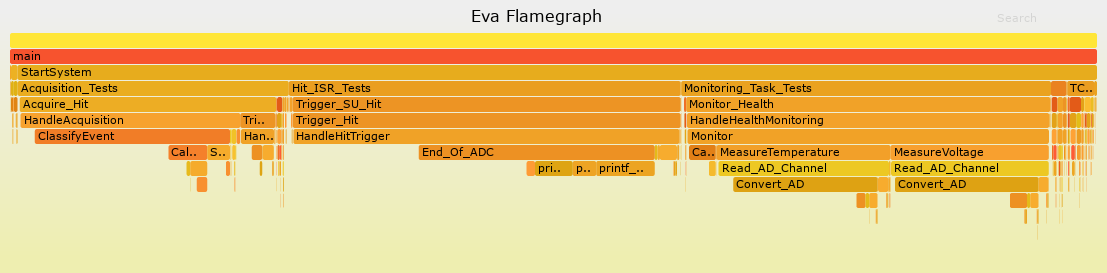
\includegraphics[width=0.95\textwidth]{flamegraph.png}
\caption{Flame graph for an analysis with Eva}
\label{fig:flamegraph}
\end{figure}

These flame graphs are interactive SVGs wrapped in an HTML page.
It is possible to zoom and filter functions by name. The length of a bar is
proportional to the time spent analyzing this function (and all other functions
called from this function). Note that if a function \texttt{f}
contains several callsites for \texttt{g}, only the total aggregated time is
displayed as a single bar \texttt{g} below \texttt{f}.
Finally, note that \texttt{-eva-flamegraph} has a negligible cost in terms of
execution time for the analysis.

\subsection{Audit messages ({\em experimental})}

Using options \lstinline|-audit-prepare| and \lstinline|-audit-check|, the
user can produce and check some information relevant for auditing purposes.

\lstinline|-audit-prepare <file>| outputs the following information:

\begin{itemize}
\item the list of all source files used during parsing: not only those
  given in the command line, but also those in \lstinline|#include|
  directives, recursively. This usually includes Frama-C's standard library.
  For each file, its MD5 checksum is also printed;
\item the list of {\em enabled} and {\em disabled} warning categories,
  for the kernel as well as for \Eva{}. Warning categories are considered
  disabled when set to one of the following actions: {\em inactive},
  {\em feedback}, and {\em feedback-once}. All other actions are considered
  as enabled;
\item the list of Eva's {\em correctness parameters}, along with their values
  at the moment when Eva is run.
\end{itemize}

The information is written to \lstinline|<file>|, in JSON format, unless it
is the special value \lstinline|-| (given as \lstinline|-audit-prepare=-|),
in which case the information is printed to the standard output in text format.

The complementary option \lstinline|-audit-check file| takes a JSON file
produced by \lstinline|-audit-prepare| and checks if all checksums, warning
category statuses and correctness parameters match. Any discrepancies are
reported and result in an error by default.

The main intent of these options is to help users perform audit-related
tasks concerning an analysis performed with Eva. It also helps fine-tuning
analyses without affecting its correctness; for instance, since it omits
information related to parameters which do not affect correctness, the user
is free to adjust them to improve the speed and precision of the analysis.

Note that these options are still in experimental stage, and should not be
blindly relied upon for strict auditing purposes. For instance, they do
not record information related to syntactic transformations performed by
plugins such as \textsf{Variadic}, which can have an indirect impact on
its correctness.

Please contact the Frama-C development team if you intend to use these
options in a production setting.

\section{About these alarms the user is supposed to check\ldots}

When writing a Frama-C plug-in to assist in
reverse-engineering source code, it does not really make sense to expect
the user to check the alarms that are emitted by \Eva{}.
Consider for instance Frama-C's slicing plug-in. This plug-in produces
a simplified version of a program. It is often applied to large unfamiliar
codebases; if the user is at the point where they need a slicer to make
sense of the codebase, it's probably a bad time to require
them to check alarms on the original unsliced version.

The slicer and other code comprehension plug-ins work around this problem
by defining the results they provide as ``valid for well-defined executions''.
In the case of the slicer, this is really the only definition that makes
sense. Consider the following code snippet:

\begin{listing}{1}
x = a;
y = *p;
x = x+1;
// slice for the value of x here.
\end{listing}

This piece of program is begging for its second line to be removed, but
if \lstinline|p| can be the \lstinline|NULL| pointer, the sliced
program behaves differently from the original: the original program
exits abruptly on most architectures, whereas the sliced version
computes the value of \lstinline|x|.

It is fine to ignore alarms in this context,
but the user of a code comprehension plug-in based on \Eva{}
should study the categorization of alarms in section \ref{obligations}
with particular care.
Because \Eva{} is more aggressive
in trying to extract precise information from the program than other
analyzers, the user is more likely to observe incorrect results if there
is a misunderstanding between him and the tool about what assumptions
should be made.

Everybody agrees that accessing an invalid pointer is an unwanted behavior,
but what about comparing two pointers with \lstinline|<=| in an undefined manner or
assuming that a signed overflow wraps around in 2's complement
representation? Function \lstinline|memmove|, for instance, typically does the
former when applied to two addresses with different bases.
%
Yet, currently, if there appears to be an undefined pointer comparison, \Eva{}
propagates a state that may contain only ``optimistic''
(assuming the undefined circumstances do not occur) results
for the comparison result and for the pointers.\footnote{As explained earlier, in this particular case, it is
possible to get all possible behaviors using option
\lstinline|-eva-undefined-pointer-comparison-propagate-all|.}

It is possible to take advantage of \Eva{}
for program comprehension, and all existing program comprehension
tools need to make assumptions about undefined behaviors. Most tools
do not tell whether they had to make assumptions or not.
\Eva{} does: each alarm, in general,
is also an assumption. Still, as implementation progresses
and \Eva{}
becomes able to extract more information from the alarms it emits,
one or several options
to configure it either not to emit some alarms, or not
to make the corresponding
assumptions, will certainly become necessary. This is a consequence
of the nature of the C language, very partially defined by a standard
that also tries to act as lowest common denominator of existing
implementations, and at the same time used for low-level programming
where strong hypotheses on the underlying architecture are needed.


\section{API}

After an analysis, most results inferred by \Eva{} can be examined in the
\FramaC graphical interface (see chapter \ref{gui}), or programmatically
accessed by another \FramaC plugin through the public \Eva{} API.

For instance, both an user (through the GUI) or a developer (through the API)
can request the evaluation of an arbitrary lvalue or expression at a given
statement.
The obtained result represents all the possible values that this lvalue or
expression may have anytime an actual execution reaches the selected statement.

\subsection{API overview}

The \Eva{} public API is available in the file \texttt{src/plugins/eva/Eva.mli}.

The function \lstinline|Analysis.compute| starts an analysis, and other
functions of the \lstinline|Analysis| module inform about the status of the
current analysis.

The \lstinline|Results| module provides access to the analysis results.
In particular, it allows the evaluation of the possible values of
arbitrary lvalues or expressions at any program point.
Such evaluation is decomposed in several steps:
\begin{enumerate}
\item first, a \lstinline|request| is built by stating where it should be
  evaluated: before or after a statement, at the start of a function, etc.
\item optionally, a request may by restricted to a given callstack;
\item then, functions \lstinline|eval_*| evaluate a variable, an lvalue or an
  expression;
\item finally, functions \lstinline|as_*| convert the evaluation result to a
  usable destination type.
\end{enumerate}

For instance, the code below evaluates the expression \lstinline|expr|
before statement \lstinline|stmt| in callstack \lstinline|cs|. The possible
values of \lstinline|expr| are expressed as an \emph{fval}, a representation
of a floating-point interval. If the evaluation fails, or if the possible values
of \lstinline|expr| cannot be represented by a floating-point interval,
\lstinline|Fval.top| is used instead.
\begin{ocamlcode}
before stmt |> in_callstack cs |>
eval_exp expr |> as_fval |> default Fval.top
\end{ocamlcode}

Other useful functions exported in the \lstinline|Results| module include:
\begin{itemize}
  \item \lstinline|callee|, which returns the list of functions that can be
    called at a given call statement, which is very useful for calls through
    function pointers.
  \item \lstinline|callers|, which returns the list of functions from which the
    given function can be called.
  \item \lstinline |is_reachable|, which returns whether a given statement has
    been reached by the analysis.
  \item \lstinline|expr_deps|, which computes an over-approximation of the
    memory zones that must be read to evaluate the given expression.
\end{itemize}

Other modules of the \Eva{} API allows to change some parameters of the
analysis, to add local annotations guiding the analysis, or to register
ocaml builtins to be used by the analysis to interpret some function calls.

The Frama-C Plug-in Development Guide contains more information about
developing a custom plug-in.

\chapter{Graphical interface (GUI)}\label{gui}
\vspace{2cm}

This chapter presents some aspects of the graphical interface of \Eva{}. More
information can be found in the Frama-C blog, under the keyword
\texttt{tutorial}.
Some examples shown in this section are taken from the Monocypher tutorial,
presented in the blog.
% The source code used in this tutorial is the version 0.3 of
% \href{http://loup-vaillant.fr/projects/monocypher/}{Monocypher}, a
% C99-conformant crytographic library that also includes a nice test
% suite\footnote{The archive for version 0.3 is available at
% \href{http://loup-vaillant.fr/projects/monocypher/monocypher-0.3.tar.gz}.}.

\begin{important}
\textbf{Note:}
This chapter describes the traditional, GTK-based graphical interface.
Frama-C is switching to {\em Ivette}, a new GUI based on Electron.
Ivette is currently under development, but it already offers most of the
existing features for viewing \Eva{} results, and also includes some new
features.

To install Ivette, you simply need to run \texttt{\em ivette} once after
installing Frama-C. This requires node v16 and yarn:
\begin{itemize}
  \item install NVM: \url{https://github.com/nvm-sh/nvm}
  \item run \texttt{\em nvm use 16}
  \item run \texttt{\em npm install --global yarn}
\end{itemize}

The following post from the Frama-C blog contains some useful information
for installing \texttt{ivette} and using it to view \Eva{} results:
\url{https://frama-c.com/2022/07/12/frama-c-25-ivette.html}

The rest of this chapter concerns the ``old'' Frama-C graphical interface.

\end{important}

\paragraph{A caveat.}

As a general recommendation,
  \textbf{do not} start your analyses within the GUI.
  Use the command-line. You should
  consider Frama-C/\Eva{} as a command-line tool with a viewer (the GUI).
  The Frama-C GUI is not an IDE (e.g.~you cannot edit code with it), and
  \Eva{} does not use the GUI for anything else other than rendering its
  results. It is recommended to run the value analysis using the command line,
  and then saving the result to a Frama-C save file
  (see Section~\ref{three-step}).

\section{A general view of the GUI}

After running the value analysis and saving your results,
it is a good time to check what the result looks like, using the GUI:

\begin{frama-c-commands}
frama-c-gui -load value.sav
\end{frama-c-commands}

In the screenshot of Figure~\ref{fig:gui-eva},
we indicate some parts of the GUI that are
useful when inspecting \Eva{} results (besides the source view). We also
indicate some parts that are never (or rarely) used with \Eva{}.

\begin{figure}[hbt]
\centering
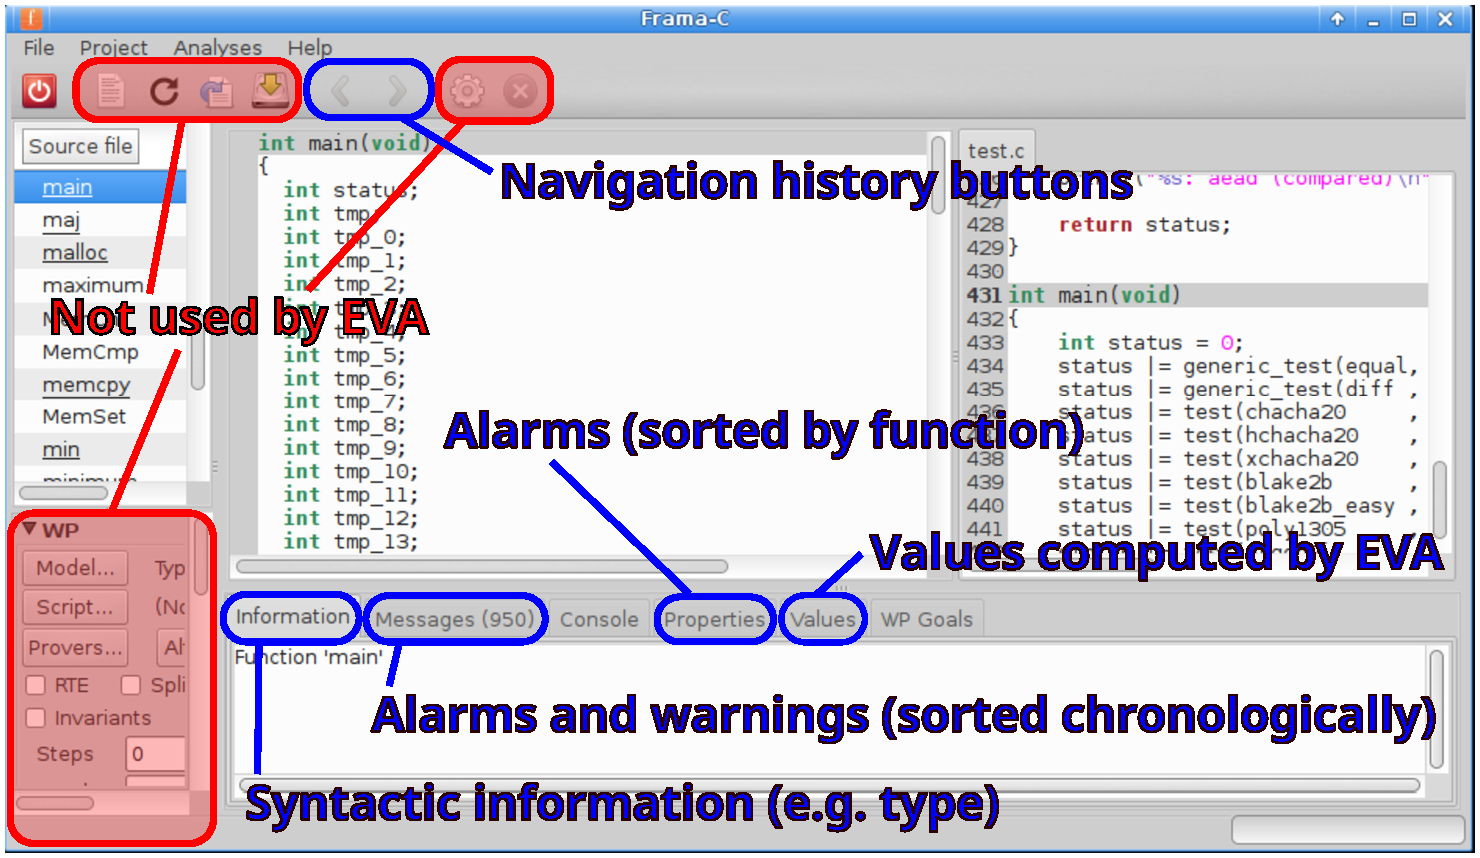
\includegraphics[width=\textwidth]{gui-images/gui1-annotated.pdf}
\caption{Frama-C GUI for \Eva{}}
\label{fig:gui-eva}
\end{figure}

Note that the Properties tab (between Console and Values) is not updated
automatically: you need to click on the \emph{Refresh} button before it
outputs anything, and after changing filters.

Like many GUI-integrated plug-ins, \Eva{} also has a side panel
that is displayed below the globals list, on the lower left corner of the GUI.
This panel can be folded/unfolded using the arrow button on the left,
and when unfolded (Figure~\ref{fig:gui-side-panel}) it displays some controls.
The {\em Run} button runs (or re-runs) the
analysis, using the specified slevel and with the specified main function.
This is useful only for small examples and rarely used in practice.
Also, notice that emitted warnings are persistent in the GUI, so even if a new
run of the value analysis (e.g.~with higher slevel) produces less alarms, the
previous warnings will still be displayed in the {\em Messages} panel.

The checkbox {\em Show list of red alarms} shows or hides the
{\em Red alarms} panel, described in Section~\ref{red-alarms}.

\begin{figure}
\centering
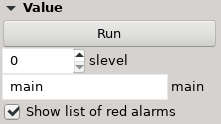
\includegraphics[scale=0.7]{gui-images/gui-side-panel.png}
\caption{GUI side panel for \Eva{}}
\label{fig:gui-side-panel}
\end{figure}


\section{Detecting and understanding non-termination}
\label{sec:non-termination-gui}

Assume that the log of your analysis contains the \texttt{NON\
  TERMINATING\ FUNCTION} message for the \texttt{main} function.
We know that
at some point in the program we will have red statements in the GUI,
which indicate unreachable code.

By scrolling down from the \texttt{main} function, we reach the
non-terminating statement, which in our example is a call to
\texttt{test\_x25519} (Figure~\ref{fig:gui-unreachable}).

\begin{figure}[hbt]
\centering
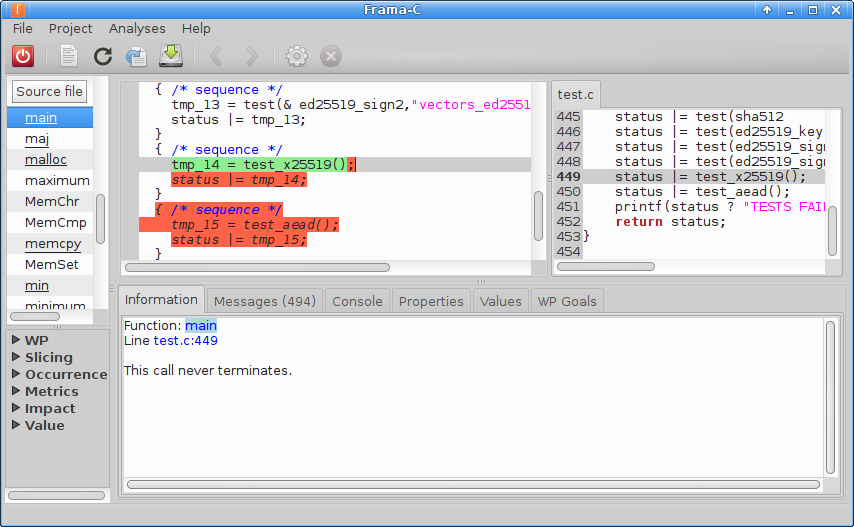
\includegraphics[width=\textwidth]{gui-images/gui2.png}
\caption{Unreachable code in the Frama-C GUI}
\label{fig:gui-unreachable}
\end{figure}

Note the red semicolon at the end of the statement, and the fact that
the statements that follow it are also red. If we click on the statement, the
\emph{Information} panel says that \emph{This call never terminates}.

You can right-click on the function and \emph{Go to the definition of
\texttt{test\_x25519}}, and you will find the same thing inside, this time a call
to \texttt{crypto\_x25519\_public\_key}, and so on, until you reach
\texttt{fe\_tobytes}, which is slightly different: it contains a
\texttt{for} loop (defined via a macro \texttt{FOR}), after which all
statements are red, but the loop itself is not an infinite loop: it
simply iterates \texttt{i} from 0 to 5. How can this be non-terminating?

The answer, albeit non-intuitive, is simple: there is one statement
inside the loop which is non-terminating, but \emph{not} during the
first iteration of the loop. Because the GUI colors are related to the
consolidated result of all callstacks (i.e., if there is at least one
path which reaches a statement, it is marked as reachable), it cannot
show precisely which callstack led to the non-termination.

% To better
% understand what happens here, we will use the \emph{Nonterm} plug-in.
% TODO

\section{Values Panel}\label{values-panel}

The Values panel, depicted in Figure~\ref{fig:values-panel}, is arguably
the most powerful inspection tool for the \Eva{} plug-in in the Frama-C GUI.

\begin{figure}[hbtp]
\centering
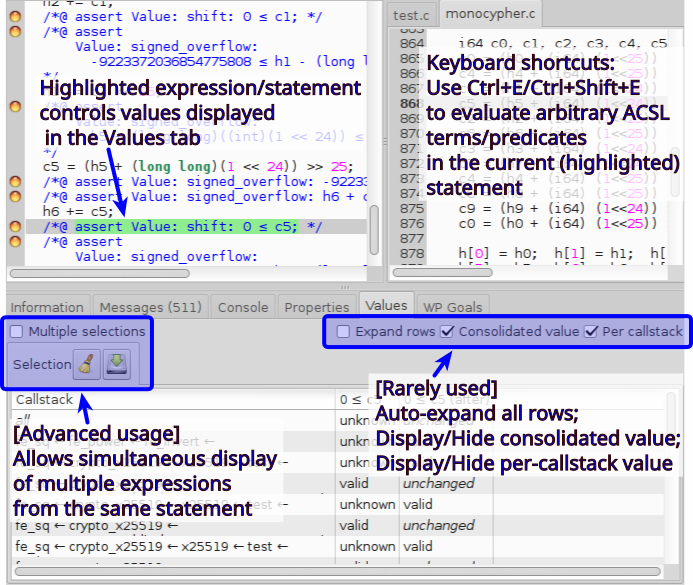
\includegraphics[width=\textwidth]{gui-images/gui-values-annotated.png}
\caption{Values panel}
\label{fig:values-panel}
\end{figure}

The values displayed in this panel are related to the green highlighted
zone in the Cil source. This zone can be a statement, an expression,
an ACSL annotation, etc. Composite expressions can be selected by clicking
on or near their operators. Each kind of selected expression has a set
of associated context menus. For instance, an expression corresponding
to a variable contains a \emph{Go to definition} context menu when
right-clicked on.

The Ctrl+E shortcut is equivalent to highlighting a statement, then
right-clicking \emph{Evaluate ACSL term}. This opens a dialog
(Figure~\ref{fig:eval-acsl}) where you can enter an arbitrary ACSL
term. Its value will be evaluated in the current statement and
displayed in the \emph{Values} panel.

\begin{figure}[!hbtp]
\centering
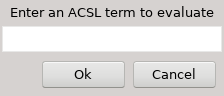
\includegraphics[scale=0.7]{gui-images/eval-acsl.png}
\caption{Evaluate ACSL term dialog, accessible via a context menu or
  by pressing Ctrl+E.}
\label{fig:eval-acsl}
\end{figure}

The Ctrl+Shift+E shortcut is slightly more powerful: it also evaluates
\emph{predicates}, such as \texttt{\textbackslash{}valid(p)}.
This command is not available from any menu.

The \emph{Multiple selections} checkbox allows adding several
expressions to be compared side-by-side. When checked, highlighting an
expression in the same statement adds a column with its value. Note that
highlighting a different statement results in resetting all columns.

The three checkboxes to the right are seldom used (their default values
are fine most of the time): \emph{Expand rows}
simply expands all callstacks (but generates visual clutter);
\emph{Consolidated value} displays the row \emph{all} (union of all
callstacks); and \emph{Per callstack} displays a row for each separate
callstack.

The callstacks display has several contextual menus that can be accessed
via right-clicks (Figure~\ref{fig:callstacks}).

\begin{figure}[hbtp]
\centering
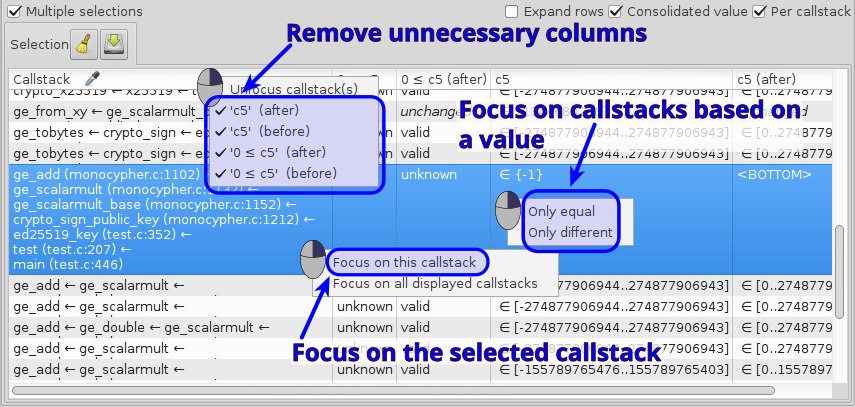
\includegraphics[width=\textwidth]{gui-images/gui-callstacks-annotated.png}
\caption{Callstacks display}
\label{fig:callstacks}
\end{figure}

Let us start from the bottom: right-clicking on a callstack shows a
popup menu that allows you to \emph{focus} on a given callstack. This
focus modifies the display in the Cil code viewer: reachability will
only be displayed for the focused callstack(s). We will come back to
that later.

Right-clicking on a cell containing a value allows filtering on all
callstacks for which the expression has the same value. This is often
used, for instance, to focus on all callstacks in which a predicate
evaluates to \emph{invalid} or \emph{unknown}.

Finally, clicking on the column headers allows filtering columns.

Note that the Callstacks column header displays a pipette icon when a
filter is being applied, to remind you that other callstacks exist.

\subsection{Filtering non-terminating callstacks}
\label{filtering-non-terminating-callstacks}

In our code, despite the existence of 40 callstacks, only one of them is
non-terminating. If you highlight the \texttt{0\ $\le$\ c5} expression
before statement \texttt{h5\ -=\ c5\ \textless{}\textless{}\ 25}, you
will see that only a single callstack displays \emph{invalid} in the
column \texttt{0\ $\le$\ c5}. Focus on this callstack using the popup menu,
then highlight expression \texttt{c5} in the Cil code. You will obtain
the result displayed in Figure~\ref{fig:non-term-callstack}.

\begin{figure}[hbt]
\centering
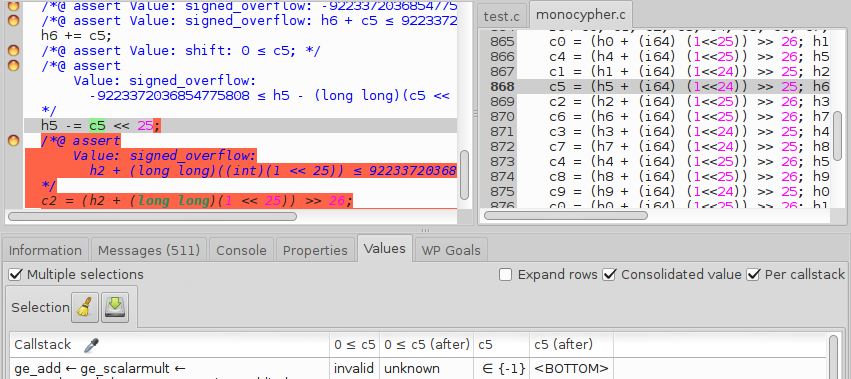
\includegraphics[width=\textwidth]{gui-images/gui5.png}
\caption{Focused on a non-terminating callstack}
\label{fig:non-term-callstack}
\end{figure}

As you can see, the GUI now displays the statements following
\texttt{h5\ -=\ c5\ \textless{}\textless{}\ 25} in red, indicating thay
they are unreachable in the currently focused callstacks. The exact
value that caused this is shown in column \texttt{c5}: \texttt{-1}. The
C standard considers the left-shift of a negative number as undefined
behavior. Because \texttt{-1} is the only possible value in this
callstack, the reduction caused by the alarm leads to a post-state that
is \texttt{\textless{}BOTTOM\textgreater{}}.

\section{Finding origins of alarms and imprecisions via the Studia plug-in}
\label{studia}

The Studia\footnote{The name \emph{Studia} is related to its applicability
to case studies.} plug-in is used to track the origins of values computed by \Eva{}.
For a given lvalue, it highlights all statements that may have written/read
it.

Studia is invoked by right-clicking on a lvalue, selecting the \emph{Studia}
menu, then the \emph{Writes} or \emph{Reads} menu (see Figure~\ref{fig:studia}).
This will highlight all the instructions that may have defined (or read)
the selected lvalue.
\emph{Studia} can also be used on arbitrary lvalues: when called through
the right-click menu with no lvalue selected, \emph{Studia} displays a
dialog box in which an arbitrary lvalue can be typed.

When a lvalue is highlighted, a new column (\emph{Studia}) appears on the
file tree. It shows a check mark next to each function that directly
writes/reads the highlighted lvalue, and an arrow next to each function
that \emph{indirectly} writes/reads the chosen value, that is, the callers of the
functions marked with a check mark.

Each statement writing/reading the chosen value is highlighted in orange in the
Cil code. Different shades of orange are used to distinguish between direct and
indirect accesses.

\begin{figure}[h!]
  \caption{\label{fig:studia}Studia elements in the GUI}
  \centering
    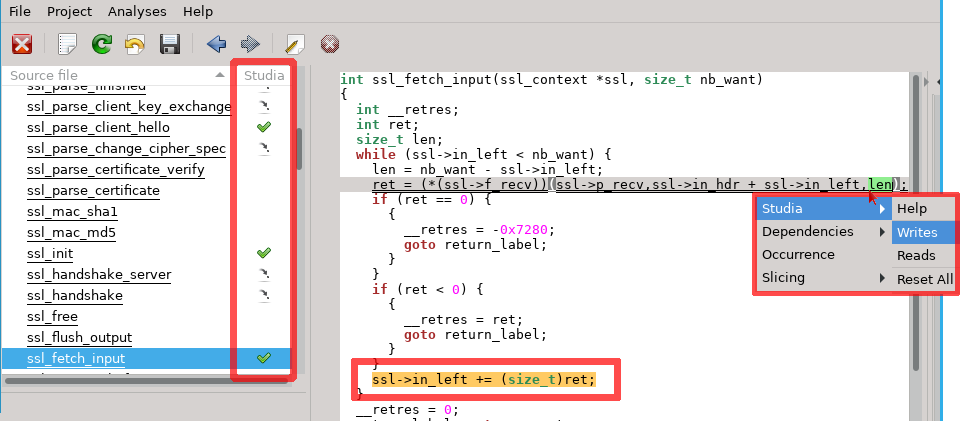
\includegraphics[width=\textwidth]{gui-images/studia}
\end{figure}

Typical usage of Studia consists in: starting the GUI, selecting an alarm
(for instance, a possibly invalid memory access), inspecting the lvalue
that causes the alarm (usually an imprecise value), then using Studia to find
where the lvalue was defined. To find the root cause of a given loss of
precision, it may be necessary to reiterate the process.

\section{Detecting branches abandoned because of red alarms}
\label{red-alarms}

When analyzing code, the value analysis sometimes encounters undefined
behaviors so severe that the analysis cannot proceed afterwards.
This is the case in the code fragment below: no state remains to be
propagated after the addition, because the uninitialized access is guaranteed.

\begin{listing-nonumber}
int x;
int y = x + 1;
\end{listing-nonumber}

This example is marked as non-terminating, both in the textual log and in
the GUI.
%
However, things are not always as clear-cut. Replace \lstinline+x+ by
a pointer access, and imagine that only in \emph{some} contexts the memory
location is uninitialized.

\begin{listing-nonumber}
void f(int *p) {
  if (rand ()) {
    int y = *p + 1;
  }
}

void main() {
  int x = 1, y;
  f(&x);
  f(&y);
}
\end{listing-nonumber}
In this example, all intructions ``terminate'' in the sense of
Section~\ref{sec:non-termination-gui}. Yet, one branch is cut abruptly
in the analysis of \lstinline+f+.

Even more insidious is a loop where an operation fails only in the last
iterations. In the example below, accessing \lstinline|t[i]| with
\lstinline|i==10| is always invalid, but this is neither reflected
in the Properties panel nor in the Values panel.

\begin{listing-nonumber}
void main() {
  int i, t[10];
  for (i=0; i<10; i++) {
    t[i] = i;
  }
  int j = 0;
  for (i=0; i<=10; i++) {
    j += t[i];
    if (rand ()) break;
  }
}
\end{listing-nonumber}

The {\em Red alarms} panel (Figure~\ref{fig:red-alarms-panel}) can be used to
detect such kinds of severe alarms.
The semantics it implements is the following: if in at least \emph{one}
analysis context, the alarm received an Invalid status (the ACSL property
does not hold), then the alarm is present in the panel.
Back to our second example, \lstinline+\initialized(p)+ is false.
The \emph{Nb contexts} column indicates in how many callstacks such an Invalid
status was emitted during the analysis.

\begin{figure}[htbp]
\centering
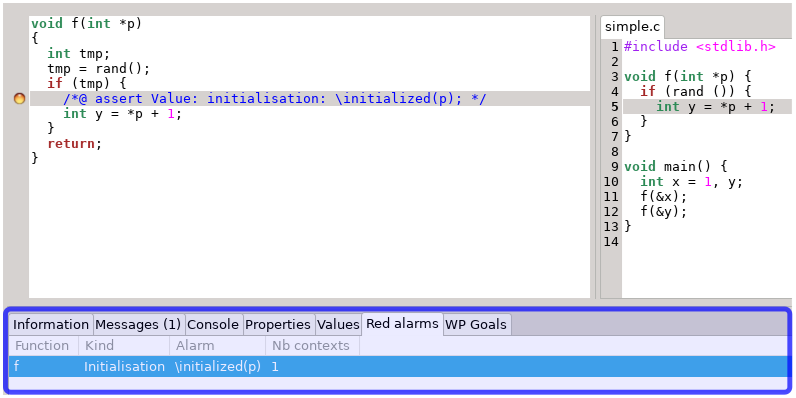
\includegraphics[width=\textwidth]{gui-images/gui-red-alarms-panel.png}
\caption{Red alarms panel}
\label{fig:red-alarms-panel}
\end{figure}

Information on non-terminating branches is also available through
the \emph{Values} panel (Figure~\ref{fig:red-values}). Once you have selected
a property listed in the \emph{Red alarms} panel, a new column appears,
which displays red indicators.
The way to read this information is: ``in this context,
the property evaluated to false at least once''.

\begin{figure}[htbp]
\centering
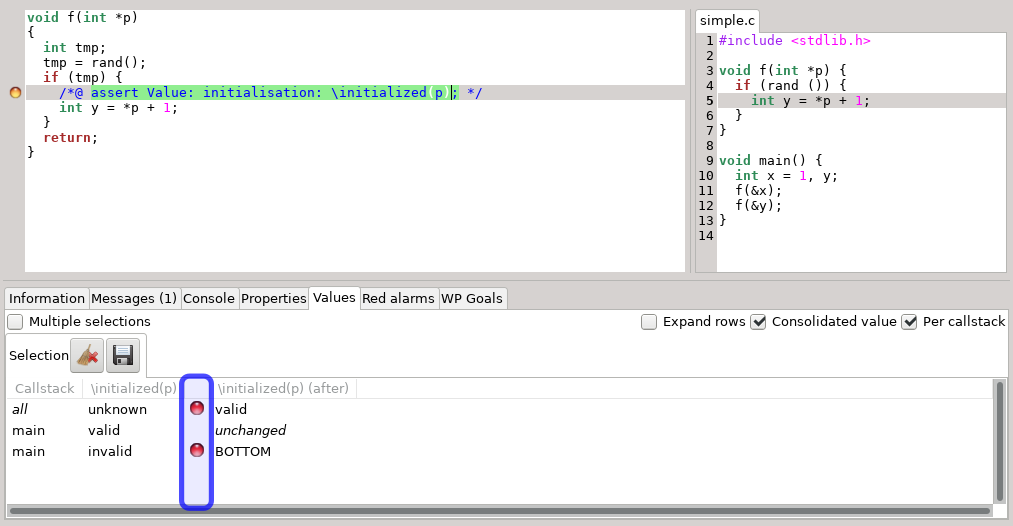
\includegraphics[width=\textwidth]{gui-images/gui-red-values.png}
\caption{Indicators of red alarms in the Values panel}
\label{fig:red-values}
\end{figure}



%% Local Variables:
%% TeX-master: "main.tex"
%% ispell-local-dictionary: "english"
%% End:


\chapter{Limitations and specificities}\label{limitations_specificities}
\vspace{2cm}

{\em Nobody is perfect.}

\vspace{2cm}

This chapter describes how the difficult constructs in the C language
are handled in \Eva{}. The constructs listed
here are difficult for all static analyzers in general.
Different static analysis techniques can often be positioned
with respect to each other by looking only at how they handle loops,
function calls and partial codebases.

\Eva{} works best on embedded code
or embedded-like code without multithreading,
although it is usable (with modeling work from the user) on
applications that include it. Dynamic allocation is supported in
limited form, but imprecisions may accumulate quickly
(e.g. linked lists often lead to suboptimal results).

\section{Prospective features}

\Eva{} does not check all the properties that could be
expected of it\footnote{There are 245 unspecified or undefined
  behaviors in Annex J of the \isoc{} standard.}. Support for each of
these missing features could arrive if the need was expressed. Below
are some of the existing limitations.

\subsection{Strict aliasing rules}

\Eva{} does not check that the analyzed program uses
pointer casts in a way that is compatible with strict aliasing
rules. This is one of the major current issues of the C world because
compilers only recently began to take advantage of these rules for
optimization purposes. However, the issue has passed unnoticed for
critical embedded code, because for various reasons including
traceability, this code is compiled with most optimizations disabled.

\subsection{Const attribute inside aggregate types}

Some memory locations can be read from but not written to.  An example
of such a memory location is a constant string literal
(\lstinline|"foo"|). The ACSL specification language sports a
predicate \lstinline|\valid_read| to express that a memory location is
valid for reading but does not have to be valid for writing.
Accordingly, \Eva{} emits alarms using
\lstinline|\valid_read(lv)| when an lvalue \lstinline|lv| is read from, and
\lstinline|\valid(lv)| when \lstinline|lv| is written to.

Variables with a const-qualified type are among the memory locations
that \Eva{} knows to be good to read from but forbidden to
write to. However, the \lstinline|const| type qualifier is currently only
handled when placed at the top-level of the type of a global variable
or formal argument. Other \lstinline|const| locations are considered
writable.

\subsection{Alignment of memory accesses}

\Eva{} currently does not check that memory accesses are
properly aligned in memory. It assumes that non-aligned accesses have
only a small time penalty (instead of causing an exception) and that the
programmer is aware of this penalty and is accessing (or seems to be accessing)
memory in a misaligned way on purpose. %% A more restrictive option
%% would be quick to implement if someone needed it. Meanwhile,
%% instructions to explicitly check for the alignment of some accesses
%% can be inserted in the code following the howto at
%% \url{http://bts.frama-c.com/dokuwiki/doku.php?id=mantis:frama-c:explicit_alignment_howto}.
% Removed: not in open-source version

%TODOBY: incomplete: many other kind of UB are not tracked

\section{Loops}
\label{boucles}

The analysis of a source program always takes a finite time.
The fact that the source code contains loops, and that some of these
loops do not terminate, can never induce the analyzer itself to loop forever.
% \footnote{An exception to this rule is when one uses the most
% precise modeling of {\tt malloc}  (details in section
% \ref{malloc}).}
In order to guarantee this property, the analyzer may need to
introduce approximations when analyzing a loop.
\medskip

Let us assume, in the following lines, that the function \lstinline|c|
is unknown:
\csource{examples/boucles.c}

The \Eva{} plug-in could provide the best possible sets of values
if the user explicitly instructed it to study step by step each
of the hundred loop iterations. Without any such instruction,
it analyses the body of the loop much less than
one hundred times. It is able to provide the approximated, but correct,
information that after the loop, \lstinline|y| contains an even number
between 0 and 256. This is an over-approximation of the most precise
correct result,
which is ``an even number between 0 and 200''.
Section \ref{boucles-traitement} introduces different ways for
the user to influence the analyzer's strategy with respect to
loops.

\section{Functions}\label{fonctions}

Without special instructions from the user, function calls are
handled as if the body of the function had been expanded at the
call site. In the following example, the body of \lstinline|f| is analyzed again
at each analysis of the body of the loop. The result of the analysis
is as precise as the result obtained for the example in section \ref{boucles}.

\csource{examples/fonctions.c}

Calls to variadic functions are handled by the \textsf{Variadic} plug-in, which
translates calls to variadic functions into semantically-equivalent calls,
either using arrays as arguments or via calls to specialized variants of the
function. Such translations are enabled by default whenever the corresponding
prototypes (e.g. \lstinline|stdio.h| for \lstinline|printf|) are included.
Calls to variadic functions in the C standard library also include
ACSL specifications, which \Eva{} uses to interpret their behavior.

Recursive functions are partially supported by \Eva{}: only a bounded
number of recursive calls can be analyzed, and a user-written specification
is required to interpret other calls.
See section \ref{recursion} for more details.

\section{Analyzing a partial or a complete application}

The default behavior of the \Eva{} plug-in allows to
analyze complete applications,
that is, applications for which the source code is entirely
available. In practice, it is sometimes desirable to limit the analysis
to critical subparts of the application, by using other entry points
than the actual one (the \lstinline|main| function).
Besides, the source code of some of the functions used by
the application may not be available (library functions for instance).
The plug-in can be used, usually with more work, in all these circumstances.
The options for specifying the entry point of the analysis are detailed
in this manual, section \ref{val-use-spec}.

\subsection{Entry point of a complete application}

When the source code for the analyzed application is entirely
available, the only additional information expected by the plug-in is
the name of the function that the analysis should start from. Specifying the
wrong entry point can lead to incorrect results. For instance, let us
assume that the actual entry point for the example of section
\ref{fonctions} is not the function \lstinline|main_1| but the following
\lstinline|main_main| function:

\listinginput{17}{examples/main.c}

If the user specifies the wrong
entry point \lstinline|main_1|, the plug-in will provide the
same answer for variable \lstinline|y| at the end of function \lstinline|f| as
in sections \ref{boucles} and \ref{fonctions}: the set of even numbers
between 0 and 256. This set is not the expected answer if the actual
entry point is the function \lstinline|main_main|, because it does not
contain the value 15.

The entry point of the analyzed application can be specified
on the command line using the option \lstinline|-main| (section \ref{entry}).
In the GUI,
it is also possible to specify the name of the entry point at
the time of launching \Eva{}.

\subsection{Entry point of an incomplete application}

It is possible to analyze an application without starting from its
actual entry point. This can be made necessary because the actual
entry point is not available, for instance if the analysis is
concerned with a library. It can also be a deliberate choice as part
of a modular verification strategy.  In this case, the option
\lstinline|-lib-entry|, described at section \ref{libentry}, should be used
together with the option \lstinline|-main| that sets the entry point of the
analysis.  In this mode, the plug-in does not assume that the global
variables have kept their initial values (except for the variables
with the \lstinline|const| attribute).

\subsection{Library functions}

Another category of functions whose code may be missing is composed
of the operating system primitives and functions from external libraries.
These functions are called ``library functions''.
The behavior of each library function can be specified through
annotations (see chapter \ref{annotations}).
The specification of a library function can in particular be
provided in terms of modified variables, and of data dependencies
between these variables and the inputs of the function
(section \ref{annot_assigns}). An alternative way to specify
a library function is to write C code that models its behavior,
so that its code is no longer missing from the point of view of the
analyzer.

Frama-C provides a set of specifications for the most common functions in the C
standard library and for some POSIX functions, plus a few extensions
(BSD, GNU, etc.). These specifications allow the analysis of applications which
use these libraries, but they become part of the {\em trusted computing base}:
it is the responsibility of the user to verify that these specifications are
correct with respect to the actual standard library implementation from the
actual execution environment.

\subsection{Choosing between complete and partial application mode}

This section uses a small example to illustrate the pitfalls that should
be considered when using \Eva{} with an incomplete
part of an application.
This example is simplified but quite typical. This is the pattern followed
by the complete application:
\begin{listing}{1}
int ok1;

void init1(void) {
  ...
  if (error condition)
    error_handling1();
  else
    ok1 = 1;
}

void init2(void) {
  if (ok1) { ... }
}

void main(void) {
  init1();
  init2();
  ...
}
\end{listing}

If \lstinline|init2| is analyzed as the entry point of a complete application,
or if the function \lstinline|init1| is accidentally omitted, then
at the time of analyzing \lstinline|init2|, \Eva{} will have no reason
to believe that the global variable \lstinline|ok1| has not kept its initial value 0.
The analysis of \lstinline|init2| consists of determining
that the value of the \lstinline|if| condition is always false, and to ignore
all the code that follows. Any possible run-time error in this function
will therefore be missed by the analyzer.
However, as long as the user is aware of these pitfalls, the analysis of
incomplete sources can provide useful results. In this example, one way
to analyze the function \lstinline|init2| is to use the
option \lstinline|-lib-entry| described in section \ref{libentry}.

It is also possible to use annotations to describe the state in which
the analysis should be started as a precondition for the entry point
function. The syntax and usage of preconditions is described in
section \ref{prepostasserts}. The user should pay attention to the
intrinsic limitations in the way \Eva{} interprets these
properties (section \ref{reduction_proprietes}). A simpler alternative
for specifying an initial state is to build it
using the non-deterministic
primitives described in section \ref{nondeterminism}.

Despite these limitations, when the specifications the user wishes to
provide are simple enough to be interpreted by the plug-in, it becomes
possible and useful to divide the application into several parts, and
to study each part separately (by taking each part as an entry point,
with the appropriate initial state). The division of the application
into parts may follow the phases in the application's behavior
(initialization followed by the permanent phase)
or break it down into elementary sub-pieces, the same way unit tests do.

\subsection{Applications relying on software interrupts}

The current version of the \Eva{} plug-in is not able to
take into account
interrupts (auxiliary function that can be executed at any time
during the main computation). As things stand, the plug-in may give
answers that do not reflect reality if interrupts play a role
in the behavior of the analyzed application.
There is preliminary support for using \Eva{} in this
context in the form of support for \lstinline|volatile| variables.

Unlike normal variables, the analyzer does not assume that
the value read from a \lstinline|volatile|
variable is identical to the last value written there. Instead,
a volatile variable in which only scalar values have been written
is assumed to contain \lstinline|[--..--]| when it is read from,
regardless of the precise value of the contents
that were previously written.
%
The values of volatile pointers ({\it i.e} variables containing pointers and
with volatile specifier)
are an imprecise form of the address that has previously been assigned to
the pointer. Finally, the handling of (non-volatile) pointers to volatile
locations is not finalized yet: it is not clear how the various complicated
situations that can arise in this case should be handled. For instance,
pointers to volatile locations may be pointing to locations that
also have non-volatile access paths to them.

\section{Conventions not specified by the ISO standard}

\Eva{} can provide useful information even for low-level
programs that rely on non-portable C construct and that depend
on the size of the word and the endianness of the target architecture.

\subsection{The C standard and its practice}
\label{norme_pratique}

There exists constructs of the C language which the ISO standard does
not specify, but which are compiled in the same way by almost every compiler
for almost every architecture. For some of these constructs, the \Eva{}
plug-in assumes a reasonable compiler and
target architecture. This design choice makes it possible to obtain more
information about the behavior of the program than would be possible
using only what is strictly guaranteed by the standard.
\medskip

This stance is paradoxical for an analysis tool whose purpose is
to compute only correct approximations of program behaviors.
Then notion of ``correctness'' is necessarily relative to a definition
of the semantics of the analyzed language. And, for the C language,
the ISO standard is the only available definition.

However, an experienced C programmer has a certain mental model of the
working habits of the compiler. This model has been acquired by
experience, common sense, knowledge of the underlying architectural
constraints, and sometimes perusal of the generated assembly code.
Finally, the Application Binary Interface may constrain the compiler
into using representations that are not mandated by the C standard
(and which the programmer should not, {\it a priori},
have counted on). Since most compilers make equivalent choices,
this model does not vary much from one programmer to the other.
The set of practices admitted by the majority of C programmers
composes a kind of informal, and unwritten, standard.
For each C language construct that is not completely specified by the
standard, there may exist an alternative, ``portable''
version. The portable version could be considered safer if the
programmer did not know exactly how the non-portable version will be
translated by their compiler. But the portable version may
produce a code which is significantly slower and/or bigger. In practice,
the constraints imposed on embedded software often lead to choosing
the non-portable version. This is why, as often as possible, \Eva{}
uses the same standard as the one used by programmers,
the unwritten one.
It is the experience gained on actual industrial software, during
the development of early versions of Frama-C as well as during
the development of other tools, that led to this choice.
\medskip

The hypotheses discussed here have to do with the conversions
between integers and pointers, pointer arithmetic, the representation
of \lstinline|enum| types and the relations between the addresses of the
fields of a same \lstinline|struct|. As a concrete example, \Eva{}
plug-in assumes two-complement representation,
which the standard does not guarantee,
and whose consequences can be seen when converting between
signed and unsigned types or with signed arithmetic overflows.
These parameters are all fixed with the \lstinline|-machdep| option
as described in section \ref{compilation}.

Often, the ISO standard does not provide enough guarantees to
ensure that the behaviors of the compiler during the compilation
of the auto-detection program and during the compilation of the application
are the same. It is the additional constraint that the compiler should conform
to a fixed ABI that ensures the reproducibility of compilation choices.

\section{Memory model -- Bases separation}\label{bases}

This section introduces the abstract representation of the memory
\Eva{} relies on. It is necessary to have
at least a superficial idea of this representation in order to
interact with the plug-in.

\subsection{Base address}
The memory model used by \Eva{} relies on the classical notion
of ``base address''. Each variable, be it local or global, defines one
and only one base address.
\goodbreak

For instance, the definitions
\begin{listing}{1}
int x;
int t[12][12][12];
int *y;
\end{listing}
define three base addresses, for \lstinline|x|,
\lstinline|t|, and \lstinline|y| respectively.
The sub-arrays composing \lstinline|t| share the same base address.
The variable \lstinline|y| defines a base address that corresponds to
a memory location expected to contain an address.
On the other hand, there is no base address for \lstinline|*y|, even
though dynamically, at a given time of the execution, it is
possible to refer to the base address corresponding to the memory
location pointed to by \lstinline|y|.

\subsection{Address}

An address is represented as an offset (which is an integer) with
respect to a base address. For instance, the addresses of the sub-arrays
of the array \lstinline|t| defined above are expressed as various offsets with
respect to the same base address.

\subsection{Bases separation}

The strongest hypothesis that the plug-in relies on is about the representation
of memory and can be expressed in this way:
{\bf it is possible to pass from one address to another through the addition
of an offset, if and only if the two addresses share the same base address}.
\medskip

This hypothesis is not true in the C language itself: addresses
are represented with a finite number of bits, 32 for instance,
and it is always possible to compute an offset to go from an address
to a second one by considering them as integers and subtracting the
first one from the second one.
The plug-in generates all the alarms that ensure, if they are checked,
that the analyzed code fits in this hypothesis. On the following example,
it generates a proof obligation meaning that ``the comparison
on line 8 is safe only if \lstinline|p| is a valid address or if the base address
of \lstinline|p| is the same as that of \lstinline|&x|''.
\csource{examples/bases.c}

It is mandatory to check this proof obligation.  When analyzing this
example, the analysis infers that the loop never terminates (because
\lstinline|p| remains an offset version of the address of \lstinline|y| and can
never be equal to the address of \lstinline|x|).  It concludes that the
only possible value for \lstinline|x| at the end of function \lstinline|main| is
2, but this answer is provided {\em proviso quod} the proof obligation
is verified through other means. Some actual executions of this
example could lead to a state where \lstinline|x| contains 3 at the end of
\lstinline|main|: only the proof obligation generated by the plug-in and
verified by the user allows to exclude these executions.
\medskip

In practice, the hypothesis of base separation is unavoidable
in order to analyze efficiently actual programs. For the programs that
respect this hypothesis, the user should simply verify the generated
proof obligations to ensure the correctness of the analysis.
For the programs that voluntarily break this hypothesis,
the plug-in produces proofs obligations that are impossible to lift:
this kind of program cannot be analyzed with the \Eva{} plug-in.

Here is an example of code that voluntarily breaks the base separation
hypothesis. Below is the same function written in the way it should
have been in order to be analyzable with Frama-C.
\begin{listing}{1}
int x,y,z,t,u;

void init_non_analyzable(void)
{
  int *p;
  // initialize variables with 52
  for (p = &x; p <= &u; p++)
    *p = 52;
}

void init_analyzable(void)
{
  x = y = z = t = u = 52;
}
\end{listing}

\subsection{Dynamic allocation}
\label{dyn-alloc}

Dynamic allocation is modeled by creating new bases.
Each call to \lstinline|malloc|/\lstinline|realloc|/\lstinline|calloc|
potentially creates a
new base, depending on the \emph{builtins} (described in section~\ref{libc})
used -- possibly resulting in an unbounded number of such bases.
Dynamically allocated bases behave mostly like statically allocated ones,
except that they come in two flavors:
%
\begin{itemize}
\item \emph{strong} bases, allocated once per call to the allocation function,
  which are precise but may cause the analysis to diverge if they are called
  inside a loop. \textbf{It is the responsibility of the user to ensure that
  strong bases are not allocated inside loops.}
\item \emph{weak} bases, allocated once per callstack, which may confound
  information from multiple calls to the allocation function, overapproximating
  their contents. This results in a less precise analysis,
  but maintains soundness and ensures termination.
  This is the safe default approach for allocations which may be nested inside
  loops.
\end{itemize}

Details about how to create and use these bases are provided in
section~\ref{malloc}.

\section{What \Eva{} does not provide}

\subsubsection{Values that are valid even if something bad happens}
\Eva{} provides sets of possible values under the
assumption that the alarms emitted during the analysis have been
verified by the user (if necessary, using other techniques).
If during an actual execution of the application,
one of the assertions emitted by \Eva{} is violated,
values other than those predicted by \Eva{} may happen.
See also questions 2 and 3 in chapter \ref{faq}.

\subsubsection{Termination or reachability properties}
Although \Eva{} sometimes detects that
a function does not terminate, it cannot be used to prove that a
function terminates. Generally speaking, the fact that \Eva{}
provides non-empty sets of values for a specific statement in
the application does not imply that this statement is reachable in a
real execution. Currently, \Eva{} is not designed to prove
the termination of loops or similar liveness properties.
For instance,
the following program does not terminate:
\csource{examples/termination.c}
If this program is analyzed
with the default options of \Eva{}, the analysis finds
that every time execution reaches the end of \lstinline|main|, the value
of \lstinline|x| is $\geq 100$. This does
not mean that the function always terminates or even that it may
sometimes terminate (it does neither). When \Eva{}
proposes an interval for \lstinline|x| at a point P,
it should always be interpreted as meaning
that {\em if P is reached, then at that time \lstinline|x| is in
the proposed interval}, and
not as implying that P is reached.

\subsubsection{Propagation of the displayed states}
The values available through the graphical and programmatic interfaces
do not come from a single propagated state but from the union of
several states that the analyzer may have propagated separately.
As a consequence, it should not be assumed that the ``state''
displayed at a particular program point has been propagated.
In the following example, \Eva{} did not emit any alarm
for the division at line 8. This means that the divisor was found never
to be null during an actual execution starting from the entry point.
The values displayed at the level of the comment should not be
assumed to imply that \lstinline|(x - y)| is never null
for arbitrary values \lstinline|x|$\in\{0;1\}$
and \lstinline|y|$\in\{0;1\}$.
\begin{listing}{1}
int x, y, z;
main(int c){
  ...
  ...
/* At this point Eva guarantees:
   x IN {0; 1}
   y IN {0; 1}; */
  z = 10 / (x - y);
}
\end{listing}
\goodbreak

With the option \lstinline|-eva-slevel| described in section \ref{slevel},
the lines leading up to this situation may for instance have been:
\begin{listing}{3}
  x = c ? 0 : 1;
  y = x ? 0 : 1;
\end{listing}

Identically, the final states displayed by the batch version of
Frama-C for each function are an union of all
the states that reached the end of the function when it was called
during the analysis.  It should not be assumed that the state
displayed for the end of a function \verb|f| is the state that was
propagated back to a particular call point. The only guarantee is
that the state that was propagated back to the call point is included
in the one displayed for the end of the function.

The only way to be certain that \Eva{} has propagated
a specific state, and therefore guarantee the absence of run-time
errors under the assumptions encoded in that state, is to build
the intended state oneself, for instance with non-deterministic
primitives (section \ref{nondeterminism}).
However, the intermediate results displayed in
the GUI can and should be used for
cross-checking that the state actually built
looks like intended.


\chapter{Parameterizing the analysis}\label{parameterizing}
\vspace{2cm}

{\em \Eva{} is automatic but gives you a little bit of control.
Just in case.}

\vspace{2cm}

Parameterization of \Eva{} involves two main kinds of options:
{\em correctness options} and {\em performance tuning options}.
The former require understanding of their meaning and of the extra hypotheses
they entail; used incorrectly, they can lead to a wrong analysis.
The latter control the tradeoff between the quality of the results and the
resources taken by the analyzer to provide them (CPU time and memory usage).
These options cannot be used wrongly, in the sense that they do not affect the
correctness of the results. However, using them efficiently is essential for
scalability of the analysis.

Section \ref{three-step} presents the overall methodology recommended when
using \Eva{}, especially for realistic code bases.
Section \ref{command-line} presents the general usage options of \Eva{} in the
command-line.
The options described in section \ref{context} are correctness options,
while the remaining sections (\ref{boucles-traitement},
\ref{trace-partitioning},
\ref{controlling-approximations} and \ref{sec:eva}) deal with performance
tuning options. Section \ref{nonterm} presents a derived analysis to
obtain information about non-termination.


\section{Three-step approach}
\label{three-step}

For realistic code bases, an analysis with \Eva{} requires several steps which
are better performed separately, for several reasons:

\begin{itemize}
\item errors are confined to each of the separate steps, instead of being
  mingled together;
\item partial results can be saved and reused, avoiding unnecessary
  recomputations;
\item it is clearer which options and changes affect which stages, leading to
  better understanding of the process.
\end{itemize}

The recommended approach can be summarized as follows:

\begin{itemize}
\item parsing sources: \verb|frama-c <sources> -save parsed.sav|;
\item running \Eva{}:  \verb|frama-c -load parsed.sav -eva -save eva.sav|;
\item viewing its results on the GUI: \verb|frama-c-gui -load eva.sav|.
\end{itemize}

The commands and options are detailed in the next section.

\section{Command line}
\label{command-line}

The parameters that determine Frama-C's behavior can be
set through the command line. There are two main variants of Frama-C,
one based on the command line (\lstinline|frama-c|), and one which launches
a graphical interface (\lstinline|frama-c-gui|).
The options understood by the \Eva{} plug-in are described in
this chapter.
All options of \Eva{} work identically for both the graphical interface
and for the command line.

\bigskip

The options documented in this manual can be listed,
with short descriptions, from the command line.
Option \lstinline|-kernel-help|
lists options that affect all plug-ins. Option
\lstinline|-eva-help| lists options specific to the
\Eva{} plug-in. The options \lstinline|-kernel-help| and
\lstinline|-eva-help| also list advanced options that are
not documented in this manual.

Example:
\begin{frama-c-commands}
frama-c -eva-help
\end{frama-c-commands}
\begin{logs}
$\dots$
-eva-slevel <n>     superpose up to <n> states when unrolling control flow.
                    The larger n, the more precise and expensive the analysis
                    (defaults to 0)
$\dots$
\end{logs}

\begin{important}
  Historically, \Eva{} was called Value, and most of its options
  were prefixed with \lstinline|-val|. All \lstinline|-val-*| options
  are aliased to equivalent \lstinline|-eva-*| functions; negative options of
  the form \lstinline|-no-val-*| are aliased to \lstinline|-eva-no-*|.
\end{important}

\subsection{Analyzed files and preprocessing}\label{sec:analyz-files-prepr}

The analyzed files should be syntactically correct C. The files
that do not use the {\tt .i} extension are automatically
preprocessed. The preprocessing command used by default is
\lstinline|gcc -C -E -I.|, but another preprocessor may be employed.

It is possible that files without a {\tt .c} extension
fail to pass this stage. It is notably the case with \lstinline|gcc|,
to which the option \lstinline|-x c| should be passed in order to preprocess
C files that do not have a \lstinline|.c| extension.
\goodbreak

Option \lstinline|-cpp-extra-args <options>| allows giving additional options
to the preprocessor, usually \verb|-D| for defining macros and \verb|-I| for
including header directories.

In rare cases, you may need to use a different preprocessing command, via
option \lstinline|-cpp-command <cmd>|.
If the patterns \lstinline|%1| and \lstinline|%2| do not appear
in the text of the
command, Frama-C invokes the preprocessor in the following way:
\begin{frama-c-commands}
<cmd> -o <outputfile> <inputfile>
\end{frama-c-commands}

In the cases where it is not possible to invoke the preprocessor with
this syntax, it is possible to use the
patterns \lstinline|%1| and \lstinline|%2|
in the command's text as place-holders for the input file (respectively,
the output file). Here are some examples of use of this option:
\begin{frama-c-commands}
frama-c-gui -eva -cpp-command 'gcc -C -E -I. -x c' file1.src file2.i
frama-c-gui -eva -cpp-command 'gcc -C -E -I. -o %2 %1' file1.c file2.i
frama-c-gui -eva -cpp-command 'copy %1 %2'  file1.c file2.i
frama-c-gui -eva -cpp-command 'cat %1 > %2' file1.c file2.i
frama-c-gui -eva -cpp-command 'CL.exe /C /E %1 > %2' file1.c file2.i
\end{frama-c-commands}

\subsection{Activating \Eva{}}

Option \lstinline|-eva| activates \Eva{}. Sets of
values for the program's variables at the end of each analyzed function
are displayed on standard output.

Many functionalities provided by Frama-C rely on \Eva{}'s
results. Activating one of these automatically activates \Eva{},
without it being necessary to provide the \lstinline|-eva|
option on the command-line.  In this case, it should be kept in mind
that all other options of \Eva{} remain available for
parameterization.

\subsection{Saving the result of an analysis}
\label{saving-result}

The option \lstinline|-save s|
saves the state of the analyzer, after the requested
computations have completed,
in a file named \lstinline|s|.
The option \lstinline|-load s| loads the state saved in file \lstinline|s|
back into memory for visualization or further computations.
\medskip

Example :
\begin{frama-c-commands}
frama-c -eva -deps -out -save result.sav file1.c file2.c
frama-c-gui -load result.sav
\end{frama-c-commands}

\begin{important}
  There is no specific extension for Frama-C saved files; the usual
  convention is to use \verb|.sav|.
\end{important}

\begin{important}
  Most options are saved when \verb|-save| is used and do not need to
  be passed again when loading it. It is therefore useful to separate
  parsing options from analysis options, the former to be saved after
  parsing, the latter to be given after loading it.
\end{important}

\subsection{Controlling  the output}

By default, \Eva{} emits all the alarms it finds (section
\ref{obligations}) as both ACSL assertions and textual messages in the
log. For big analyses, the log can become quite large. Since ACSL
assertions are stored by the Frama-C kernel, and can be output using
plugins such as Report, the textual output is partly redundant. Warning
category\footnote{See Frama-C User Manual~\cite{FCUserMan}.}
\texttt{alarm} allows to manage how these alarms are reported on the
textual output. In particular, \texttt{-eva-warn-key alarm=inactive} will
completely disable their output, and \texttt{-eva-warn-key alarm=feedback}
will convert them into normal messages instead of warnings
(equivalent to deprecated option
\texttt{-eva-no-warn-on-alarms}\footnote{Note that the use of
  \texttt{-eva-no-warn-on-alarms -eva-msg-key=-alarm} for completely
  deactivating the output will not work anymore, as \texttt{alarm} is not a
  debug category anymore.}).

\section{Describing the analysis context}
\label{context}

\subsection{Specification of the entry point}
\label{entry}

The option \lstinline|-main f| specifies that \lstinline|f| should be
used as the entry point for the analysis. If this option is
not specified, the analyzer uses the function called \lstinline|main|
as the entry point.

\subsection{Analysis of a complete application}
\label{complete}

By default (when the option \lstinline|-lib-entry| is {\em not} set),
the analysis starts from a state
in which initialized global variables
contain their initial values, and uninitialized ones contain zero.
This only makes sense if the entry point (see section \ref{entry}) is
the actual starting point of this analyzed application.
In the initial state, each formal argument of the entry point contains
a non-deterministic value that corresponds to its type. Representative
locations are generated for arguments with a pointer type,
and the value of the pointer argument is the union of the address
of this location and of \lstinline|NULL|. For chain-linked structures,
these locations are allocated only up to a fixed depth.

Example: for an application written for the POSIX interface, the
prototype of \lstinline|main| is:
\cwithrange{1-1}{examples/parametrizing/simple-main.c}
The types of arguments \lstinline|argc| and \lstinline|argv|
translate into the following initial values:
\logwithrange{8-14}{examples/parametrizing/simple-main.log}

This is generally not what is wanted, but then again, embedded applications
are generally not written against the POSIX interface. If the analyzed
application expects command-line arguments, you should probably
write an alternative entry point that creates the appropriate context
before calling the actual entry point.
That is, consider an example application whose source code looks like this:
\begin{listing-nonumber}
int main(int argc, char **argv)
{
  if (argc != 2) usage();
  ...
}

void usage(void)
{
  printf("this application expects an argument between '0' and '9'\n");
  exit(1);
}
\end{listing-nonumber}

Based on the informal specification provided in \lstinline|usage|,
you should make use of the non-deterministic primitives described in
section \ref{nondeterminism} to write an alternative entry point
for the analysis like this:
\begin{listing-nonumber}
int eva_main(void)
{
  char *argv[3];
  char arg[2];
  arg[0]=Frama_C_interval('0', '9');
  arg[1]=0;
  argv[0]="Analyzed application";
  argv[1]=arg;
  argv[2]=NULL;
  return main(2, argv);
}
\end{listing-nonumber}

For this particular example, the initial state that was
automatically generated includes the desired one. This may however
not always be the case. Even when it is the case, it is desirable
to write an analysis entry point that positions the
values of \lstinline|argc| and \lstinline|argv| to
improve the relevance of the alarms emitted by \Eva{}.

Although the above method is recommended for a complete
application, it remains possible to let the analysis automatically
produce values for the arguments of the entry point. In this
case, the options described in section \ref{generation_initial} below
can be used to tweak the generation of these values to some extent.

\subsection{Analysis of an incomplete application}\label{libentry}

%see examples/parametrizing/global-initial-value.c

The option \lstinline|-lib-entry| specifies that the analyzer should not use
the initial values for globals (except for those qualified
with the keyword \lstinline|const|).
With this option, the analysis starts with an initial state
where the numerical components of
global variables (without the \lstinline|const| qualifier) and arguments
of the entry point are initialized with a non-deterministic value of their
respective type.

Global variables of pointer type contain the non-deterministic
superposition of \lstinline|NULL| and of the addresses of
locations allocated by the analyzer. The algorithm to generate
those is the same as for formal arguments of the entry point (see previous
section). The same options can be used to parameterize the generation of
the pointed locations (see next section).

\subsection{Tweaking the automatic generation of initial values}
\label{generation_initial}

This sections describes the options that influence
the automatic generation of initial values
of variables. The concerned
variables are the arguments of the entry point and,
in \lstinline|-lib-entry| mode, the non-const global variables.

\subsubsection{Width of the generated tree}

For a variable of a pointer type, there is no way for the analyzer
to guess whether the pointer should be assumed to be pointing to a single
element or to be pointing at the
beginning of an array --- or indeed, in the middle of an array, which
would mean that it is legal to take negative offsets of this pointer.

By default, a pointer type is assumed to point at the beginning
of an array of two elements. This number can be changed with option
\lstinline|-eva-context-width|.

Example: if the prototype for the entry point is \lstinline|void main(int *t)|,
the analyzer assumes \lstinline|t| points to an array \lstinline|int S_t[2]|.

For an array type, non-aliasing subtrees of values
are generated for the first
few cells of the array. All remaining cells are made to contain a
non-deterministic superposition of the first ones. The number
of initial cells for which non-aliasing subtrees are generated is
also decided by the value of option \lstinline|-eva-context-width|.

Example: with the default value \lstinline|2| for option
\lstinline|-eva-context-width|, the declaration \lstinline|int *(t[5]);|
causes the following array to be allocated:
\logwithrange{8-13}{examples/parametrizing/context-width.log}

Note that for both arrays of pointers and pointers to pointers,
using option \lstinline|-eva-context-width 1| corresponds to a very strong
assumption on the contents of the initial state with respect to aliasing.
You should only use the argument \lstinline|1| for
option \lstinline|-eva-context-width| in special cases, and use at least
\lstinline|2| for generic, relatively representative calling contexts.

\subsubsection{Depth of the generated tree}

For variables of type pointer to pointers, the analyzer limits the depth up
to which initial chained structures are generated.
This is necessary for recursive types such as follows.
\cwithrange{1-1}{examples/parametrizing/context-depth.c}
This limit may also be observed for non-recursive types if they are deep enough.

Option \lstinline|-eva-context-depth| allows to specify this limit.
The default value is 2. This number is the depth at which
additional variables named \lstinline|S_...| are allocated, so
two is plenty for most programs.

For instance, here is part of the initial state displayed by \Eva{}
in \lstinline|-lib-entry| mode if a global variable \lstinline|s|
has the type \lstinline|struct S| defined above:
\logwithrange{4-15}{examples/parametrizing/context-depth.1.log}

In this case, if variable \lstinline|s| is the only one which
is automatically allocated, it makes sense to set the option
\lstinline|-eva-context-width| to one.  The value of the
option \lstinline|-eva-context-depth| represents the length of the
linked list which is modeled with precision. After this depth,
an imprecise value (called a well) captures all the possible continuations
in a compact but imprecise form.

Below are the initial contents for a variable \lstinline|s| of type \lstinline|struct S|
with options \lstinline|-eva-context-width 1|
\lstinline|-eva-context-depth 1|:

\logwithrange{4-14}{examples/parametrizing/context-depth.2.log}

\subsubsection{The possibility of invalid pointers}

In all the examples above, \lstinline|NULL| was one of the
possible values for all pointers, and the linked list that was
modeled ended with a well that imprecisely captured all continuations
for the list. Also, the \lstinline|context-width| parameter
for the generated memory areas has to be understood as controlling the maximum
width for which the analyzer assumes the pointed area may be valid.
However, in order to assume as little as possible on the calling context
for the function, the analyzer also
considers the possibility that any part of the pointed area might \emph{not} be
valid. Thus, by default, any attempt to access such an area results in an alarm
signaling that the access may have been invalid.\footnote{For technical
reasons, this also means that it is not possible to reduce the values
of those areas through user-provided assertions
(section~\ref{reduction_proprietes}).
}

The option \lstinline|-eva-context-valid-pointers| causes
those pointers to be assumed to be valid (and
\lstinline|NULL| therefore to be omitted from the possible values)
at depths that are less than the context width.
It also causes the list to end with a
\lstinline|NULL| value instead of a well.

When analyzed with options
\lstinline|-eva-context-width 1| \lstinline|-eva-context-depth 1|
\lstinline|-eva-context-valid-pointers|,
a variable \lstinline|s| of
type \lstinline|struct S| receives  the following initial contents,
modeling a chained list of length exactly 3:

\logwithrange{4-9}{examples/parametrizing/context-depth.3.log}

\subsection{State of the IEEE 754 environment}

The IEEE 754 standard specifies a number of functioning modes for
the hardware that computes floating-point operations. These modes
determine which arithmetic exceptions can be produced and rounding
direction for operations that are not exact.

By default, obtaining an
infinite or NaN as result of a floating-point operation is treated
as an unwanted error. Consequently, FPU modes related to arithmetic
exceptions are irrelevant for the analysis.
For non-default values of option \texttt{-warn-special-float}, the
behavior of changing the floating-point environment is currently unspecified.

% \Eva{} currently offers two models of the
% floating-point hardware's rounding mode. Depending on the program analyzed
% and the compiler used, one of the following situations may occur.

The compilation of, and the set of floating-point operations used, define
roughly three categories of programs:
\begin{enumerate}

\item The program uses only
\lstinline|double| and \lstinline|float| floating-point types,
does not change the default (nearest-even) floating-point rounding
mode and is compiled with a compiler that neither generates
\lstinline|fmadd| instructions nor generates extended precision computations
(historical x87 instruction set).
% It can be analyzed with the default
% modeling of floating-point rounding.

\item The compiler transforms floating-point computations
as if floating-point addition or multiplication were associative,
or transforms divisions into a multiplication by the inverse even when
the inverse cannot be represented exactly as a floating-point number.
% This case is not supported by \Eva{}.

\item The program uses only
\lstinline|double| and \lstinline|float| floating-point types,
but either does not stay during the whole
execution in the ``nearest'' floating-point rounding mode, or is
compiled with a compiler that may silently insert \lstinline|fmadd|
instructions when only multiplications and additions appear in the
source code, or are compiled for the x87 FPU. % It can be analyzed
% correctly by using the \lstinline|-all-rounding-modes| analysis option.
\end{enumerate}
%
Currently, only programs of the first category can be soundly analyzed by
\Eva{}.

% The \lstinline|-all-rounding-modes| option forces the analyzer to take
% into account more behaviors. The results obtained may therefore seem
% less precise with this option. Still, the user must resist the temptation
% to analyze eir program without this option when ey is not in the
% conditions that allow it, because the analysis may then be incorrect
% (the analysis may fail to predict some behaviors of the analyzed program, and
% for instance fail to detect some possible run-time errors).

\subsection{Setting compilation parameters} \label{compilation}

\subsubsection{Using one of the pre-configured target platforms}

The option \lstinline|-machdep |{\it platform}
sets a number of parameters for the low-level description of the
target platform, including the
\emph{endianness} of the target and size of each C type.
The option \lstinline|-machdep help| provides a list of currently supported
platforms. The default is \lstinline|x86_64|, an AMD64-compatible processor with
what are roughly the default compilation choices of gcc.

\subsubsection{Targeting a different platform}

If your target platform  is not listed,
please contact the developers.
An auto-detection program can be provided in order to check the hypotheses
mentioned in section~\ref{norme_pratique}, as well as to detect the
parameters of your platform.
It comes under the form of a C program of a few lines, which should ideally be
compiled with the same compiler as the one intended to compile the
analyzed application. If this is not possible, the analysis can also be
parameterized manually with the characteristics of the target
architecture.
The Frama-C Plugin Development Guide~\cite{plugin-dev-guide} contains a
section about customizing the machine model.

\subsection{Parameterizing the modeling of the C language}

The following options are more accurately described as
pertaining to Frama-C's modeling of the C language
than as a description of the target platform, but of course
the distinction is not always clear-cut. The important thing to remember
is that these options, like the previous one, are dangerous options
that should be used, or omitted, carefully.

\subsubsection{Valid absolute addresses in memory}

By default, \Eva{} assumes that the absolute addresses in
memory are all invalid. This assumption can be too restrictive,
because in some cases there exist a limited number of absolute
addresses which are intended to be accessed by the analyzed program,
for instance in order to communicate with hardware.

The option \lstinline|-absolute-valid-range m-M|
specifies that the only valid absolute addresses (for reading or writing)
are those comprised between \lstinline$m$ and \lstinline$M$ inclusive.
This option currently allows to specify only a single interval,
although it could be improved to allow several intervals
in a future version.


\subsubsection{Overflow in array accesses}
\label{unsafe-arrays}

\Eva{} assumes that when an array
access occurs in the analyzed program, the intention is that the
accessed address should be inside the array. If it can not determine that
this is the case, it emits an \lstinline|out of bounds index|
alarm. This leads to an alarm on the following example:
\csource{examples/parametrizing/out-of-bound.c}
\Eva{} assumes that writing \lstinline|t[0][...]|, the programmer
intended the memory access to be inside \lstinline|t[0]|. Consequently,
it emits an alarm:
\logwithrange{5-6}{examples/parametrizing/out-of-bound.log}
The option \lstinline|-unsafe-arrays| tells \Eva{} to warn
only if the address as computed using its modeling of pointer arithmetics
is invalid. With the option, \Eva{} does not warn about line 4
and assumes that the programmer
was referring to the cell \lstinline|t[1][2]|.

The default behavior is stricter than necessary but often produces more
readable and useful alarms. To reiterate, in this default behavior
\Eva{} gets hints from the syntactic shape of the program.
Even in the default mode, it does not warn for the following code.
\begin{listing}{4}
  int *p=&t[0][12];
  return *p;
}
\end{listing}

Option \lstinline|-safe-arrays| also has an effect on the evaluation
of the ACSL construct ``\lstinline|..|''. When \lstinline|t| is a
known array, \lstinline|t[..]| is strictly equivalent to
\lstinline|t[0..s-1]|, where \lstinline|s| is the number of elements
of \lstinline|t|. Conversely, when option \lstinline|-unsafe-arrays| is
set, \lstinline|t[..]| means
\lstinline|t[-|$\infty$\lstinline|..+|$\infty$\lstinline|]| -- meaning
that the location overlaps with neighbouring zones when \lstinline|t| is
inside an array or struct.

\subsection{Dealing with library functions}

When the \Eva{} plug-in encounters a call to a library
function, it may need to make assumptions about the effects of this call.
The behavior of library functions can be described precisely
by writing a contract for the function (chapter \ref{annotations}),
especially using an \lstinline|assigns| clause (section \ref{annot_assigns}).

If no ACSL contract is provided for the function, the analysis uses the
type of the function as its source of information for making
informed assumptions. However, no guarantee is made that those assumptions
over-approximate the real behavior of the function. The inferred
contract should be verified carefully by the user.

\subsection{Analyzing recursive functions}
\label{recursion}

By default, recursive calls are not analyzed; instead, \Eva{} uses the
specification written by the user for the recursive function to interpret
its recursive calls. The analysis of the function is then incomplete,
as only its non-recursive calls are analyzed: values are inferred and
alarms are emitted only for these calls.
For the recursive calls, the analysis' soundness relies entirely on the
specification provided by the user, which is not verified, and a warning
is emitted.

\begin{logs}
[eva] file.c: Warning:
  Using specification of function <name> for recursive calls.
  Analysis of function <name> is thus incomplete and its soundness
  relies on the written specification.
\end{logs}

If no ACSL contract is provided for the recursive function,
a minimal specification is inferred by the \FramaC kernel
from the function type, and an error is emitted.
The specification is only generated to allow the analysis to continue
past the recursive call, without any guarantees that it describes correctly
the real behaviors of the function.
In particular, only \lstinline|assigns| clauses are created, without any
preconditions.
It is the user's responsibility to replace this generated specification by
a correct one.

\subsubsection{Unrolling recursive calls}

Option \lstinline|-eva-unroll-recursive-calls n| allows the precise analysis
of recursive calls up to a depth of <n>. The function specification is only used
when encountering a recursive call of depth greater than <n>.

On the example below, analyzed with \lstinline|-eva-unroll-recursive-calls 10|:
\begin{itemize}
\item
  the first call \lstinline|factorial(8)| is soundly and precisely analyzed
  without any warnings;
\item
  the analysis of the second call \lstinline|factorial(20)| is incomplete and
  produces a warning, as it resorts to the function specification for the tenth
  recursive call.
\end{itemize}

\csource{examples/parametrizing/recursion-simple.c}

With option \lstinline|-eva-unroll-recursive-calls|,
the analysis of a recursive function can thus be complete and sound,
when the number of recursive calls can be bounded by the analysis.
In that case, no ACSL specification is required for the analysis of the
recursive function.

However, even when the number of recursive calls is bounded in practice,
the \Eva{} analysis might be too imprecise to be complete.

\csource{examples/parametrizing/recursion-imprecise.c}

The above example presents a recursive function \lstinline|mod3|, which
computes the congruence modulo 3 in up to three recursive calls.
However, Eva is unable to perform a complete analysis of this function
in the general case and will instead rely on the \lstinline|mod3| specification,
as it cannot reduce the new argument value of the recursive calls, as shown
by the successive values printed by the \lstinline|Frama_C_show_each| directive:

\logwithrange{10-17}{examples/parametrizing/recursion-imprecise.log}

Finally, note that the unrolling of a very large number of recursive calls can
considerably slow down the analysis.


\subsection{Using the specification of a function instead of its body}
\label{val-use-spec}

In some cases, one can estimate that the analysis of a given function \verb+f+
takes too much time. This can be caused by a very complex
function, or because \verb+f+ is called many times during the analysis.
Another situation is when a function already has a functional specification,
proved for instance with the \textsf{WP} plug-in, and we do not want/need
to analyze it with \Eva{}.

In the cases above, a somewhat radical
approach consists in replacing the entire body of the function
by an ACSL contract that describes its behavior. See for example
section~\ref{annot_assigns} for how to specify which values the function
reads and writes.

Alternatively, one can leave the body of the function untouched, but
still write a contract. Then it is possible to use the option
\verb+-eva-use-spec f+. This instructs \Eva{} to use the
specification of \verb+f+ instead of its body each time a call to
\verb+f+ is encountered. This is equivalent\footnote{Except for a few
  properties, as described in the next paragraph.} to deleting the body
of \verb+f+ for \Eva{}, but not for the other plug-ins of \FramaC,
that may study the body of \verb+f+ on their own.

Notice that option \verb+-eva-use-spec f+ loses some guarantees. In particular,
the body of \verb+f+ is not studied at all by \Eva{}. Neither
are the functions that \verb+f+ calls, unless they are used by some other
functions than \verb+f+. Moreover, \Eva{} does not attempt
to check that \verb+f+ conforms to its specification. In particular,
postconditions are marked as {\em unknown} with \verb+-eva-use-spec+,
while they are {\em considered valid} for functions without body.
It is the responsibility
of the user to verify those facts, for example by studying \verb+f+
on its own in a generic context.



%\section{Controlling approximations}
%
%Unlike options of section \ref{context}, which used wrongly may cause
%\Eva{} to produce incorrect results, all the options
%in this section give the user control over the tradeoff between the
%quality of the results and the resources taken by the analyzer to
%provide them. The options described in this section can, so to speak,
%not be used wrongly. They may cause Frama-C to exhaust the available
%memory, to take a nearly infinite time, or, in the other direction,
%to produce results so imprecise that they are useless, but {\bf never}
%to produce incorrect results.

\section{Improving precision in loops}
\label{boucles-traitement}

The default treatment of loops by the analyzer often produces
results that are too approximate.
Fine-tuning loops is one of the main ways to improve precision in the analysis.

When encountering a loop, the analyzer tries to compute a state
that contains all the possible concrete states at run-time,
including the initial concrete state just before entering the loop.
This enclosing state, by construction, is often imprecise:
typically, if the analyzed loop is initializing an array,
the user does not expect to see the initial values of
the array appear in the state computed by the analyzer.
The solution in this case is to either unroll loops, using one of several
available methods, or to add annotations (widening hints or loop invariants)
that enable the analyzer to maintain precision while ensuring the analysis
time remains bounded.

\subsection{Loop unrolling}
\label{loop-unroll}

Whenever a loop has a fixed number of iterations (or a known upper bound),
Eva can precisely analyze it by semantically unrolling each iteration,
avoiding merging states from different iterations.
This leads to increased cost in terms of analysis, but usually the cost
increase is worth the improvement in precision.

Loop unrolling is often easy to apply, since it does not require much
knowledge about the loop, other than an estimate of the number of iterations.
If the estimate is too low, precision won't improve; if it is too high,
it may lead to unnecessary work; but under no circumstances will it affect the
correctness of the analysis.

\subsubsection{Automatic loop unrolling}

\Eva{} includes a syntactic heuristic to automatically unroll simple loops
whose number of iterations can be easily bounded.
It is enabled via option \lstinline|-eva-auto-loop-unroll <n>|, where
\lstinline|<n>| is the maximum number of iterations to unroll: loops with
less than \lstinline|<n>| iterations will be completely unrolled.
If the analysis cannot infer that a loop terminates within less than
\lstinline|<n>| iterations, then no unrolling is performed.

\lstinline|-eva-auto-loop-unroll| is recommended as the first approach towards
loop unrolling, due to its low cost and ease of setup. An unrolling limit
up to a few hundred seems suitable in most cases.

If \emph{all} loops in a program need to be unrolled, one way to do it quickly
consists in using option \lstinline|-eva-min-loop-unroll <n>|,
where \lstinline|<n>| is the number of iterations to unroll in each loop.
This option is very expensive, and its use should be limited.

For a more fine-grained analysis and for non-trivial loops,
annotations are available to configure the loop unrolling on a case by case
basis.
These annotations take precedence over the automatic loop unrolling mechanism
and can be combined with them, e.g. to automatically unroll {\em all but} a few
loops.

With options \lstinline|-eva-auto-loop-unroll AUTO -eva-min-loop-unroll MIN|:
\begin{itemize}
\item if a loop has a loop unroll annotation, it is unrolled accordingly;
\item otherwise, if a loop has evidently less than \lstinline|AUTO| iterations,
  it is completely unrolled;
\item otherwise, the \lstinline|MIN| first iterations of the loop are unrolled.
\end{itemize}

\subsubsection{Loop unroll annotations}

Individual loops can be unrolled by preceding them with a
\lstinline|loop unroll <n>| annotation, where \lstinline|<n>| is the number
of iterations to unroll.
Such annotations must be placed just before the loop (i.e. before the
\lstinline|while|, \lstinline|for| or \lstinline|do| introducing the loop),
and one annotation is required per loop, including nested ones. For instance:

\csource{examples/parametrizing/loop-unroll-const.c}

The annotations above will ensure
that \Eva{} will unroll the loops and keep the analysis precise; otherwise,
the array access \lstinline|a[i][j]| might generate alarms due to imprecisions.

The \lstinline|loop unroll| parameter can be any C expression evaluated to a
single integer value by \Eva{} each time the analysis reaches the loop.
Otherwise, the annotation is ignored and a warning is issued.
Constants obtained via \lstinline|#define| macros, variables which always have
a unique value and arithmetic operators are suitable.
For expressions that have several possible values,
the acceptability of the annotation depends on the precision of the analyzer.
Note that there are interesting cases of non-constant expressions for
unrolling annotations. The example below shows a function with two nested loops.

\csource{examples/parametrizing/loop-unroll-nested.c}

The number of iterations of the outer loop is constant while the number of
iterations of the inner loop depends on the current iteration of the outer
one. As we have instructed \Eva{} to unroll the outer loop, it evaluates the
parameter \lstinline|sizes[i]| to a single possible integer for each iteration
of the outer loop, and thus the inner loop annotation is accepted. In this
example, it is also possible to use an upper bound like $4$.

The unrolling mechanism is independent of \lstinline|-eva-slevel|
(see next subsection): annotated loops are always unrolled at least the specified
number of times. If the loop has not been entirely unrolled, however,
remaining \lstinline|-eva-slevel| may be used to unroll more iterations.

While it is sometimes useful to unroll only the first iterations, the usual
objective is full unrolling; for this reason, the user is informed whenever
the specified unrolling value is insufficient to unroll the loop entirely:

\csource{examples/parametrizing/loop-unroll-insuf.c}

\logwithrange{5-5}
  {examples/parametrizing/loop-unroll-insuf.log}

The message can be disabled via \lstinline|-eva-warn-key loop-unroll=inactive|.

Note that using an unrolling parameter which is higher than the actual number
of iterations of a loop doesn't generally have an effect on the analysis.
The analyzer will usually detect that further iterations are not useful.

Loop annotations can also be used to prevent the automatic loop unrolling
for some specific loops: adding \lstinline|loop unroll 0| before a loop
ensures that no iteration of the loop will be unrolled.

\subsubsection{Unrolling via option {\em -eva-slevel}}
\label{slevel}

The option \lstinline|-eva-slevel n| indicates that the analyzer is allowed
to separate, in each point of the analyzed code,
up to \lstinline|n| states from different execution paths before starting
to compute the unions of said states. An effect of this option
is that the states corresponding to the first, second,\ldots
iterations in a loop remain separated, as if the loop had been unrolled.

Unlike with \lstinline|loop unroll| annotations, the number \lstinline|n|
to use with \lstinline|-eva-slevel| depends on the nature of the control flow
graph of the function to analyze.
If the only control structure is a loop of \lstinline|m| iterations,
then \texttt{-eva-slevel \textsf{m+1}} allows to unroll the loop completely.
The presence of other loops or of \lstinline|if-then-else| constructs
multiplies the number of paths a state may correspond to,
and thus the number of states it is necessary to keep separated
in order to unroll a loop completely.
For instance, the
nested simple loops in the following example require the
option \lstinline|-eva-slevel 55| in order to be completely unrolled:
\csource{examples/parametrizing/slevel.c}

When the loops are sufficiently unrolled, the result obtained for the
contents of array \lstinline|t| are the optimally precise:
\logwithrange{11-11}{examples/parametrizing/slevel.1.log}

The number to pass the option \lstinline|-eva-slevel|  is of the magnitude of
the number of values for \lstinline|i| (the 6 integers between 0 and 5)
times the number of possible values for \lstinline|j| (the 11
integers comprised between 0 and 10). If a value much lower than
this is passed, the result of the initialization of array \lstinline|t|
will only be precise for the first cells. The option \lstinline|-eva-slevel 28|
gives for instance the following result for array \lstinline|t|:
\logwithrange{12-13}{examples/parametrizing/slevel.2.log}

In this result, the effects of the first iterations of the loops
(for the whole of \lstinline|t[0]|, the whole of \lstinline|t[1]| and the first
half of \lstinline|t[2]|) have been computed precisely. The
effects on the rest of \lstinline|t| were computed with
approximations. Because of these approximations, the analyzer can not
tell whether each of those cells contains 1 or its original value 0.
The value proposed for the cells \lstinline|t[2][5]| and following
is imprecise but correct. The set \lstinline|{0; 1}| does
contain the actual value \lstinline|1| of the cells.

The option \lstinline|-eva-slevel-function f:n| tells the analyzer to apply
semantic unrolling level \lstinline|n| to function \lstinline|f|.
This fine-tuning option allows to
force the analyzer to invest time precisely analyzing functions that matter,
for instance \lstinline|-eva-slevel-function crucial_initialization:2000|.
Oppositely, options \lstinline|-eva-slevel 100 -eva-slevel-function trifle:0|
can be used together to avoid squandering resources over irrelevant parts of
the analyzed application. The \lstinline|-eva-slevel-function| option can be used
several times to set the semantic unrolling level of several functions.

Overall, \lstinline|-eva-slevel| has the advantage of being quick to setup.
However, it is in many cases superseded by \lstinline|-eva-precision|, which
controls other parameters related to analysis precision and speed.
Also, \lstinline|-eva-slevel| does not allow fine grained control as
loop unrolling annotations,
it is context-dependent (e.g. for nested loops), unstable (minor changes in
control flow may affect the usage of slevel) and hard to estimate in presence
of complex control flows.

\subsubsection{Syntactic unrolling}

Syntactic unrolling (option \lstinline|-ulevel n|, provided by the \FramaC
kernel), while not recommended when using \Eva{}, is another way to unroll
loops for a more precise analysis. The only advantage of syntactic unrolling
is that the GUI will show separate statements, allowing
the user to see the values of variables at each iteration.
However, this method is slower and leads to code which may become less
readable, due to the introduction of extra variables, labels and statements.

The value \lstinline$n$ is the number of times to unroll the loop before starting
any analysis (if larger than the number of loop iterations, the extra code will
still be generated, but it may end up being considered unreachable by \Eva{}).
In any case, a large value for \lstinline|n| makes the analyzed code larger,
especially for nested loops. This may cause the analyzer to use more time and
memory.

It is possible to control syntactic unrolling for each loop in the analyzed code
with the annotation \lstinline|//@loop unfold n;|, placed before the loop.
You may also specify \lstinline|//@loop unfold "completely", n;| for a loop
that shall be completely unrolled after $n$ steps. Although, consider that
a loop that executes $n$ times before exiting will need $n+1$ unrolling steps,
since the $n+1$ iteration need to be executed for terminating the loop.

\subsection{Widening hints and loop invariants}

Besides loop unrolling, another technique to improve precision in loops
consists in using the standard computation by accumulation mechanism present in
tools based on abstract interpretation. This mechanism requires a more involved
setup, but can lead to more efficient analyses.

As compared to loop unrolling, the advantage of the computation
by accumulation is that it generally requires less iterations
than the number of iterations of the analyzed loop. The number of
iterations does not need to be known (for instance, it allows to
analyze a \lstinline|while| loop with a complicated condition).
In fact, this method can be used even if the termination of
the loop is unclear. These advantages are obtained thanks to
a technique of successive approximations. The approximations
are applied individually to each memory location in the state.
This technique is called ``widening''.
Although the analyzer uses heuristics to figure out the best
parameters in the widening process, it may (rarely) be appropriate
to help it by providing it with the bounds that are likely to
be reached, for a given variable modified inside a loop.

\subsubsection{Widening hints}
\label{subsub:widen-hints}

The user may place an annotation \lstinline|//@ widen_hints $v$, $e_1,\ldots,e_m$ ;|
to indicate the analyzer should use preferably the values $e_1,\ldots,e_m$
when widening the sets of values attached to variable $v$.

Example:
\csource{examples/parametrizing/widen-hints.c}

$e_1,\ldots,e_m$ (the hint \emph{thresholds}) must evaluate to compilation-time
constants. They may contain numeric expressions and reference preprocessor
macros and \lstinline|const int| variables.
Note that several hints can be added to a single statement, as follows:

\begin{listing-nonumber}
  /*@ widen_hints x, 10, 20, 30;
      widen_hints y, 5, 25; */
\end{listing-nonumber}

The user may also annotate a loop with
\lstinline|//@ loop widen_hints $v$, $e_1,\ldots,e_m$ ;|,
in which case $v$ may reference loop iteration variables.

Adding a \lstinline|global| label before the variable name, as in
\lstinline|//@ loop widen_hints global:n, $e_1,\ldots,e_m$ ;|,
makes the annotation affect all loops in all functions, including
those from other compilation units. It is useful for referencing variables
in inner loops whose outer loop is defined in another file.

Finally, the user may replace the variable name with \lstinline|"all"|
(including the double quotes) to apply the widening hints to {\em all} variables.

Note that these annotations affect {\em all} statements in the function,
including statements {\em preceding} the one where the annotation is inserted.

\subsubsection*{Dynamic widening hints}

\lstinline|widen_hints| annotations accept not only variables, but more
generally \emph{lvalues}, such as \lstinline|*p| and \lstinline|a[i]->p|.
If the lvalue contains a dereference operator, then the widening hint is
considered \emph{dynamic}: it is applied to every base pointed to by the lvalue
at the statement where the hint is applied. In other words, if the hint
\lstinline|*p, 42| is inside a loop, and at each loop iteration \lstinline|*p|
may point to a new base, then each new base has 42 added to its widening
thresholds.

Dynamic hints are automatically global; the \lstinline|global| prefix must not
be applied to them.

\subsubsection{Loop invariants}

A last technique consists in using the loop invariant construct of ACSL.
Loop invariants describe some
properties that hold at the beginning of each execution of a loop,
as explained in the ACSL specification, \S2.4.2.
%\url{http://frama-c.com/download/acsl.pdf}
%
They can be used to gain precision when analyzing loops in
the following way: when the analysis is about to widen the value of a
variable, it intersects the widened domain with the one inferred through
the loop invariant. Thus, the invariant can be used to limit the
(possibly overly strong) approximation induced by the widening step.

\begin{listing}{1}
#define N 10

void main (int c)
{
  int t[N+5];
  if (c >= 1 && c < N)
  {
    int *p=t;
    /*@ loop invariant p < &t[N-1]; */
    while(1)
    {
      *(++p) = 1;
      if(p >= t+c)
        break;
    }
  }
}
\end{listing}
In the example above, without a loop invariant, the pointer \lstinline+p+
is determined to be in the range \lstinline|&t + [4..60],0%4|. In C terms, this
% <<do not fix the above even if it is wrongly colorized by Emacs. It is right>>
means that \lstinline+p+ points between \lstinline+&t[0]+
and \lstinline+&t[15]+, inclusive. In particular, the analysis is not able
to prove that the access on line~9 is always valid.

Thanks to the loop invariant \lstinline|p < &t[N-1]|, the variable
\lstinline+p+ is
instead widened to the range \lstinline+&t[0]..&t[N-2]+.
This means that the access to \lstinline+t+
through \lstinline+p+ at line 7 occurs
within bounds\footnote{And more precisely between \lstinline+t[1]+ and
\lstinline+t[9]+, since \lstinline+p+
is incremented before the affectation to \lstinline+*p+.}.
Thus, this technique is complementary to the use of
\lstinline+widen_hints+, which only accepts integers --- hence not
\lstinline+&t[N-1]+. Compared to the use
of \lstinline+-eva-slevel+ or \lstinline+-ulevel+,
the technique above does not unroll the loop; thus the overall results
are less precise, but the analysis can be faster.

Notice that, in the function above, a more precise loop invariant would be
\begin{listing-nonumber}
/*@ loop invariant p < &t[c-1]; */
\end{listing-nonumber}
However, this annotation cannot be effectively used by \Eva{}
if the value for \lstinline+c+ is imprecise, which is the case in our
example. As a consequence, the analysis cannot prove this improved invariant.
We have effectively replaced an alarm, the possible out-of-bounds access at
line~7, by an invariant, that remains to be proven.


\section{Improving precision with case-based reasoning}
\label{trace-partitioning}

Some formal proofs about programs require to use \emph{case-based reasoning}.
\Eva{} can perform such reasonings through \emph{trace partitioning}
\cite{trace-partitioning} techniques, which can be enabled globally or
by specific annotations. It is important to note that, whatever the method used,
a partitioning (and thus the case-based reasoning) currently stops at the end of
a function, and can only be extended past the function return if there is enough
\lstinline|slevel| in the calling function.


\subsection{Automatic partitioning on conditional structures}

It sometimes happens that the cases we want to reason on are exactly the
cases distinguished in the program by an \lstinline|if-then-else| statement or a
\lstinline|switch| not far above, even if these blocks are already closed
at the point we need the case-based reasoning. Unless enough
\lstinline|slevel| is available, the cases of a conditional structure are
approximated together as soon as the analyzer leaves the block. However, \Eva{}
can delay this approximation until after the statement where the case-based
reasoning is needed.

The global command-line parameter \lstinline|-eva-partition-history <n>|
delays the approximation for all conditional structures of the whole
program. The parameter \lstinline|<n>| controls the delay:
it represents the number of junction points for which the incoming
paths (the cases) are kept separated. At a given point, \Eva{} is then able to
reason by cases on the \lstinline|<n>| last \lstinline|if-then-else| statements
closed before.
A value of $1$ means that \Eva{} will reason by
case on the previous \lstinline|if-then-else|, until another one is closed.

This option has a very high cost on the analysis, theoretically doubling the
analysis time for each increment of its parameter $n$.
The cost can even be higher on \lstinline|switch| statements.
However, it can remove false alarms in a fully automatic way. Thus,
the trade off might often be worth trying.

In practice, \lstinline|-eva-partition-history 1| seems to be sufficient in
most cases, and a greater value is rarely needed.


\subsection{Value partitioning}
\label{value-partitioning}

\subsubsection{Principle}

A case-based reasoning on the possible values of an expression can be forced
inside a function by using \lstinline|split| annotations.  These annotations
must be given an expression whose values correspond to the cases that need to be
enumerated. The example below shows a use of this annotation.

\csource{examples/parametrizing/split-array.c}

The \lstinline|split| instructs \Eva{} to enumerate all the possible
values of \lstinline|i| and to continue the analysis separately for
each of these values. Thereafter, the value of \lstinline|i| is always
evaluated by \Eva{} as a singleton in each case, which enables the use of a
\lstinline|loop unroll| annotation on \lstinline|i|. This way, the result of
the function can be exactly computed as the set of three possible values instead
of an imprecise interval.

\logwithrange{22-23}{examples/parametrizing/split-array.log}

A \lstinline|split| annotation can be used on any expression that evaluates to a
{\it small} number of integer values. In particular, the expression can be a C
comparison like in the following example.

\csource{examples/parametrizing/split-fabs.c}

This example requires the equality domain (enabled with option
\lstinline|-eva-domains equality|, see section \ref{sec:symbolic-equalities}) to
be analyzed precisely, as we need the equality relations between the input and
the output of the function \lstinline|fabs|, i.e. the relations
\lstinline|x == \result| or \lstinline|x == -\result|.
Then, the \lstinline|split| annotation before the call to \lstinline|fabs|
allows \Eva{} to reason by case and to infer the relevant equality in each case.

This example also illustrates the use of a \lstinline|merge| annotation, which
ends the case-based reasoning started by a previous \lstinline|split| annotation
with the exact same expression.
The use of \lstinline|merge| annotations is not mandatory, but they allow the
user to mitigate the cost of \lstinline|split| annotations.

\subsubsection{Static and dynamic partitioning}

Two kinds of value partitioning are available:
\begin{description}
\item[Static split] with annotation \lstinline|//@ split e;| \\
  The partitioning is done once at the annotation point: Eva enumerates all
  possible values of the given expression, and continues the analysis separately
  for each of these values, until a merge annotation is encountered.
\item[Dynamic split] with annotation \lstinline|//@ dynamic_split e;| \\
  The partitioning is maintained at each program point according to the current
  value of the given expression \lstinline|e|. At each assignment of a variable
  on which \lstinline|e| depends, the partitioning is updated to ensure that the
  expression always evalutes to a singleton in each analysis state, until a
  merge annotation is encountered.
\end{description}

A static split allows reasoning according to the value of an expression at the
annotation point, while a dynamic split enables reasoning according to the
current value of the expression as long as the partitioning is active.

In both following examples, the values of the array \lstinline|t| are sorted in
increasing order, so the value of \lstinline|t[i+1] - t[i]| is always positive.
However, without value partitioning, the analysis computes independently the
possible values for \lstinline|t[i]| and \lstinline|t[i+1]|, which may have
any value in the intervals $[0..55]$ and $[1..89]$ respectively,
and \lstinline|r = t[i+1] - t[i]| may then be negative.

To be precise on these examples, we need to separate the analysis for each value
of \lstinline|i|, so that the accesses to the values of \lstinline|t| are exact.
With such partitioning, the values of \lstinline|t[i]|, \lstinline|t[i+1]| and
\lstinline|r| are computed separately for each possible value of \lstinline|i|.

\csource{examples/parametrizing/static-split.c}

To be precise on this first example, we need a static split on \lstinline|i|, as
the value of \lstinline|i| is set to 0 before the computation of \lstinline|r|,
but the values of \lstinline|x| and \lstinline|y| depend on the previous value
of \lstinline|i|.

\csource{examples/parametrizing/dynamic-split.c}

In this second example, the value of \lstinline|r| is computed at each
loop iteration and depends on the current value of \lstinline|i|, which
also changes at each loop iteration.
So we need a dynamic split to ensure that the analysis separates the new
values of \lstinline|i| during the analysis of the loop.

We could also use a static split in the loop body, to ensure that the
partitioning is updated at each loop iteration. On more complex codes where
the partitioned value is written or used many times, a single dynamic split
is often more suitable than static splits.



\subsubsection{Interprocedural value partitioning}

By default, the value partitioning performed by \lstinline|split|
and \lstinline|dynamic_split| annotations is only maintained in the current
function: when returning to the caller, the value partitioning
finishes and partitioned states are merged together.

The option \lstinline|-eva-interprocedural-splits| can be used to change this
behavior and keep value partitioning through return statements.

Alternatively to annotations, it is also possible to use the command line to
perform case-based reasoning throughout the whole analysis. The command-line parameter
\lstinline|-eva-partition-value <v>| forces the analyzer to reason at all times
on single values of the global variable \lstinline|v|, by performing a
dynamic split on \lstinline|v| for the whole analysis.

\subsubsection{Limitations}

There are four limitations to the value partitioning:

\begin{enumerate}
\item Splits can only be performed on integer expressions. Pointers and
  floating-point values are not supported yet.
\item The expression on which the split is done must evaluate to a small set of
  integer values, in order to limit the cost of the partitioning and ensure the
  termination of the analysis. If the number of possible values inferred for the
  expression exceeds a defined limit, \Eva{} cancels the split and emits a
  warning. The limit is 100 by default and can be changed with option
  \lstinline|-eva-split-limit <n>|.
\item While the number of simultaneous splits (whether local with annotations
  or global through command line) is not bounded, there can be only one split
  per expression. If two \lstinline|split| annotations use the same expression,
  only the latest one encountered on the path will be kept. Although it is a
  limitation, it can be used to define strategies where a case-based reasoning
  is controlled accross the whole program.
\item When the expression is complex, the ability of \Eva{} to reason
  precisely by cases depends on the enabled abstract domains (see section
  \ref{sec:eva}) and their capability to learn from the value of the expression.
  If \Eva{} detects that the expression is too complex for the split to be useful,
  it will cancel the split and warn the user.
\end{enumerate}


\section{Controlling approximations}
\label{controlling-approximations}

\subsection{Cutoff between integer sets and integer intervals}

Option \verb|-eva-ilevel <n>| is used to indicate the number of elements
below which sets of integers should be precisely represented as sets.
Above the user-set limit, the sets are represented as intervals
with periodicity information, which can cause approximations.

Example:
\csource{examples/parametrizing/ilevel.c}

With the default limit of 8 elements for sets of integers, the
analysis of the program shows a correct but approximated result:

\logwithrange{20-20}{examples/parametrizing/ilevel.1.log}

Studying the program, the user may decide to improve the precision of
the result by adding \verb|-eva-ilevel 16| to the command line. The
analysis result then becomes:

\logwithrange{20-20}{examples/parametrizing/ilevel.2.log}

\subsection{Maximum number of precise items in arrays}

Option \verb|-eva-plevel <n>| is used to limit the number of elements
in an array that can be considered precisely during assignments.
When assigning a value to an array element, if the index is imprecise,
it may be very costly to update each array element individually.
Instead, if the range of indices to be accessed is larger than {\em plevel},
some approximations are made and a message is emitted:

\begin{listing-log}
[kernel:approximation] arrays.c:32:
  more than 200(300) locations to update in array. Approximating.
\end{listing-log}

This message means that the array to be updated had 300 elements, and
\verb|-eva-plevel| was set to 200 (the default value). In this case, it
might be reasonable to increase the plevel to 300, especially if some alarms
could be caused by the imprecision. In other cases, however, there is little
hope of obtaining a reasonable bound:

\begin{listing-log}
more than 200(0x20000000) locations to update in array. Approximating.
\end{listing-log}

In some cases, lowering the plevel can improve performance, but it is rarely
a significant factor. Most of the time, this option has little impact in the
analysis, both in terms of precision and performance. However, when dealing
with large arrays and matrices, it is worth considering its usage.


\subsection{Subdividing the evaluation of non-linear expressions}
\label{subdividing-evaluation}

Option \verb|-eva-subdivide-non-linear| improves the analysis precision on
non-linear expressions, such as \lstinline|x * x|,
or on any expression with multiple occurrences of the same lvalue.

The interval semantics is inherently imprecise on non-linear expressions.
When $x \in [-10..10]$, the interval semantics computes $x*x \in [-100..100]$.
Subdivisions can mitigate this imprecision by splitting the evaluation of
\lstinline|x*x| according to the possible values of \lstinline|x|,
and then joining the results.
When \verb|-eva-subdivide-non-linear| is enabled, \Eva{} evaluates the
expression \lstinline|x*x| separately for $x \in [-10..0]$ and $x \in [0..10]$,
and computes the precise interval $x*x \in [0..100]$ for both cases.
On this example, splitting the values of x further would not improve the result.

The argument of \verb|-eva-subdivide-non-linear| is the maximal number of
subdivisions that can be performed for each non-linear expression.
This limit is not always reached, as heuristics may detect when more
subdivisions cannot lead to a better result.
This option slightly slows down the analysis, as more computations are performed;
in practice, the limit can usually be set up to several hundreds even on
large programs.

The option is global, and subdivisions are applied to any non-linear expression
of integer or floating-point type.
Subdivisions can also be controlled locally by writing annotations
in the analyzed code:
a \lstinline|//@  subdivide N;| annotation instructs \Eva{}
to apply up to $N$ subdivisions when evaluating the following statement,
regardless of option \verb|-eva-subdivide-non-linear|.

Finally, \Eva is also able to subdivide the evaluation of an expression
according to the values of an arbitrary number of lvalues;
thus, this subdivision mechanism can also improve the precision on expressions
that are non-linear on several lvalues, such as \lstinline|x*x - 2*x*y + y*y|.

\section{Analysis domains}
\label{sec:eva}

This section presents the analysis \emph{domains}
available to improve the precision on specific code constructs.
They can (and probably should) be enabled at the beginning of the analysis.
Their only downside is that they increase the analysis time.

Figure~\ref{fig:eva-domains} presents the list of currently available analysis
domains, with a short description of each one.
Most domains are also presented in more details in the following subsections.

\begin{figure}
  \begin{tabular}{lll>{\raggedright}m{7.5cm}}
    Name & Log & Ref & Description\tabularnewline
    \midrule
    \midrule
    cvalue & d-cvalue &  &
    Main analysis domain, enabled by default. Should not be disabled.
    \tabularnewline
    \midrule
    equality & d-equality & \ref{sec:symbolic-equalities} &
    Infers equalities between C expressions. \\
    Useful on most analyses and very efficient.
    \tabularnewline
    \midrule
    symbolic-locations & d-symbolic-locations & \ref{sec:reuse} &
    Infers values at symbolic locations. \\
    Useful on most analyses and very efficient.
    \tabularnewline
    \midrule
    gauges & d-gauges & \ref{sec:gauges} &
    Infers linear inequalities between variables modified within a loop. Efficient.
    \tabularnewline
    \midrule
    octagon & d-octagon & \ref{sec:octagons} &
    Infers relations of the form $l \leq \pm X \pm Y \leq u$ between integer or
    pointer lvalues. Efficient.
    \tabularnewline
    \midrule
    multidim & d-multidim & \ref{sec:multidim} &
    More precise representation of arrays of structures,
    multidimensional arrays and arrays invariants.
    Experimental.
    \tabularnewline
    \midrule
    bitwise & d-bitwise & \ref{sec:bitwise} &
    Interprets more precisely some bitwise operations. Rarely useful.
    \tabularnewline
    \midrule
    sign & d-sign &  &
    Infers the sign of variables. Rarely useful.
    \tabularnewline
    \midrule
    apron-box & d-apron-box & \multirow{5}{*}{\ref{sec:apron}} &
    \multirow{5}{7.5cm}{Experimental and often costly. \\
      Binding to the Apron library domains.}\tabularnewline
    apron-octagon & d-apron-octagon &  & \tabularnewline
    apron-polka-equality & d-apron-polka-equality &  & \tabularnewline
    apron-polka-loose & d-apron-polka-loose &  & \tabularnewline
    apron-polka-strict & d-apron-polka-strict &  & \tabularnewline
    \midrule
    taint & d-taint & \ref{sec:taint} &
    Experimental. Performs a taint analysis.
    \tabularnewline
    \midrule
    numerors & d-numerors & \ref{sec:numerors} &
    Experimental. Infers ranges for absolute and relative errors
    in floating-point computations.
    \tabularnewline
    \midrule
    inout & d-inout &  &
    Experimental. Computes the input and output of each function.
    \tabularnewline
    \midrule
    traces & d-traces &  &
    Experimental. Builds an over-approximation of all traces leading to
    a statement.
    \tabularnewline
    \midrule
    printer & d-printer &  & Only useful for developers.
    \tabularnewline
    \bottomrule
  \end{tabular}

  \caption{Analysis domains \label{fig:eva-domains}}
\end{figure}

These analysis domains are enabled by the option \texttt{-eva-domains}, followed
by a list of domain names. A list of the available domains, and a short
description of each one, can be displayed with \texttt{-eva-domains help}.

Domains can also be enabled for specific functions through option
\texttt{-eva-domains-function}:
\begin{itemize}
\item \texttt{-eva-domains-function d1:f,d1:g,d2:h} enables the domain
  \texttt{d1} on functions \lstinline+f+ and \lstinline+g+, and the domain
  \texttt{d2} on function \lstinline+h+.
\item \texttt{-eva-domains-function d:f+} enables the domain
  \texttt{d} on function \lstinline+f+ and on any function called
  from \lstinline+f+.
\item \texttt{-eva-domains-function d:f-} disables the domain
  \texttt{d} on function \lstinline+f+ and on any function called
  from \lstinline+f+.
\end{itemize}

These analysis domains currently have some restrictions:
\begin{itemize}
\item adding a new domain may interact with the \lstinline+slevel+ partitioning
  in unpredictable ways, and new alarms may sometimes appear;
\item the properties inferred by these domains cannot be easily viewed in the
  GUI; only a few domains have their values printed in the \emph{Values} tab.
\end{itemize}

However, the properties inferred by a specific domain at a program point may be
inspected by using the directive \lstinline+Frama_C_dump_each+ or
\lstinline+Frama_C_domain_show_each+ in the analyzed source code, and by
enabling the log category of the given domain. These directives are described
in Section~\ref{buitins_observation}, and the log category of each domain
is given by Figure~\ref{fig:eva-domains}.

\subsection{Symbolic equalities}
\label{sec:symbolic-equalities}

Activating option \texttt{-eva-domains equality} instructs
\Eva{} to perform a special analysis that stores information
about equalities found in the code. Those equalities may stem either
from conditions (e.g. \texttt{if (x == y+1)}), or assignments
\texttt{y = x+2;}. Once an equality has been inferred, it will
be used when one of the expressions involved occurs later in the program.


\begin{listing-nonumber}
  int y = x+1;
  // the equality y == x + 1 is inferred
  if (y <= 2) {
    // Thanks to the equality, x <= 1 is deduced
  }
}
\end{listing-nonumber}

This domain should be activated by default. Indeed, the normalisation
done by \FramaC for expressions with side-effects introduces temporary
variables, for which the equality domain is useful to regain
precision.

By default, the analysis is partially inter-procedural.
At the end of a call, equalities inferred in the called function are always
propagated back to the caller.
At the beginning of a call, the option \verb+-eva-equality-through-calls+
controls which equalities from the caller are propagated to the called function.
Three global modes are available:
\begin{description}
\item[none] No equality is propagated to called functions. Faster but less
  precise mode.
\item[formals] Default mode: only the equalities between the formal parameters
  and the actual arguments of the call are used at the beginning
  of a function.
\item[all] All equalities from the call site are used when analyzing a called
  function.  This slows down the analysis, and should only be set for specific
  functions through the option \verb+-eva-equality-through-calls-function+.
\end{description}


\subsection{Reused left-values}
\label{sec:reuse}

Activating option \texttt{-eva-domains symbolic-locations} instructs
\Eva{} to perform a special analysis for \emph{reused left-values}.

\begin{listing-nonumber}
int t[10];

extern unsigned int u[10];

//@ requires i < 10;
void main(unsigned int i) {
  if (u[i] < 8) {
    t[u[i]] = 2;
  }
}
\end{listing-nonumber}
On this code, \Eva{} cannot represent precisely \lstinline+u[i]+, and
``learns'' nothing from the condition \lstinline+u[i] < 8+. Hence, \Eva{}
emits an alarm on the line \lstinline|t[u[i]] = 2|, as it cannot prove
that \lstinline+u[i]+ is less than 10.

To allow learning information from such conditionals,
the new analysis stores information especially for \texttt{u[i]} itself.
This analysis is of course correct in presence of pointers, in particular
when the left-value is written through an alias between two read accesses.
All ``compound'' left-values such as \texttt{u[i]}, \texttt{*p} or
\texttt{q->t[i].v} are handled.

Currently, the analysis is intra-procedural. The information known
in the caller is not propagated in the callee.

\subsection{Gauges}
\label{sec:gauges}

Activating option \texttt{-eva-domains gauges} instructs \Eva{} to
store relations between integer (or pointer) variables modified by a
loop, and the number of elapsed loop iterations. It is based on the
paper \emph{``The Gauge Domain: Scalable Analysis of Linear
Inequality Invariants''}
\cite{DBLP:conf/cav/Venet12}.


\begin{listing-nonumber}
int y = 3;
int t[100];
int *p = &t[0];

for (int i=0; i<100; i++) {
  y += 2; // y == 2*i + 5 holds. In particular, y <= 203
  *p++ = i; // all accesses are in bound
}
\end{listing-nonumber}

This domain should be activated for programs in which finite loops
increase multiple variables simultaneously, in an affine way. It
is \emph{not} useful if the loop is fully unrolled by syntactic or
semantic means, or if the relation between
variables is not affine (e.g. computing a square).

\begin{listing-nonumber}
  if (x++ <= 10) { ... }

// Transformed into

  int tmp = x;
  x++;
  if (tmp <= 10) { // Nothing is learnt on x without the
                   // domain of equalities }
\end{listing-nonumber}

Currently, the analysis is intra-procedural only: no information
flows from the caller to the callee, or in the reverse direction.
The relations inferred can only involve variables that are:
\begin{itemize}
\item local to a function (e.g. not a global), and not \texttt{static};
\item scalar (not a field of a struct, or a cell in an array).
\end{itemize}

Beware that the analysis works better when arithmetic overflows
are reported as an alarm. With the default options of \FramaC,
this means that gauges can be inferred easily for \emph{signed}
variables, but less so for \emph{unsigned} ones. Indeed, the affine
relations inferred by the domain are no longer true once the
variable exceeds e.g. \texttt{INT\_MAX} and wraps. Code such as
\begin{listing-nonumber}
unsigned int x = ...;
int y = ...;

while (--x > 0) {
  y++;
  [...]
}
\end{listing-nonumber}
 cannot be analyzed precisely, because the relation between \texttt{x}
and \texttt{y} is not affine.


\subsection{Octagons}
\label{sec:octagons}

Activating option \texttt{-eva-domains octagon} instructs Eva to infer relations
between variables as numerical constraints of the form $l \leq \pm X \pm Y \leq
u$, where $X$ and $Y$ are program variables or lvalues,
and $l$ and $u$ are constants.

These relations are then used to evaluate more precisely the possible values
of an expression involving $X$ and $Y$, or to deduce a reduction of
the possible values of $X$ from a reduction of the possible values of $Y$.

The following code is a minimal working example that illustrates
the precision improvement provided by the octagon domain.
\begin{listing-nonumber}
void main (int y) {
  int k = Frama_C_interval(0, 10);
  int x = y - k;               // y - x $\in$ [0..10]
  int r = x + 3 - y;           // r $\in$ [-7..3]
  int t;
  if (y > 15)
    t = x;                     // t $\in$ [6..$\infty$]
}
\end{listing-nonumber}


Currently, the octagon domain is fast but has some limitations:
\begin{itemize}
\item
  The domain only infers relations between lvalues of integer or
  pointer types.
  It does not support relations between floating-point values.
\item
  The domain only infers relations between pairs of variables occurring in the
  same instruction, as \lstinline|x = y + k;| or \lstinline|if (x < y + k)|.
  If an instruction involves 3 variables or more, relations are inferred for
  each pair of variables.
\item
  The domain has no involved memory model and can only infer and use relations
  about the syntactic lvalues as they appear in the program.
  For instance, if two pointers \lstinline|p| and \lstinline|q| point to the
  same location, and a relation is inferred on \lstinline|*p|, the domain cannot
  use it to improve the value of \lstinline|*q|.
\end{itemize}

The domain is intraprocedural by default: the inferred relations are local to
the current function and are lost when entering a function call or returning
to its caller.

The option \verb+-eva-octagon-through-calls+ makes the octagon domain
interprocedural, which is a more precise but slower mode where
the inferred relations are propagated through function calls.
The analysis of a function can then use the relations previously inferred in the
callers, and at the end, the inferred relations are propagated back to the
caller.


\subsection{Multidim}
\label{sec:multidim}

\emph{This domain is experimental.}

The multidim domain implements a typed memory model designed to abstract
multidimensional arrays, arrays of structures, or any composition of any depth
of these. It can also infer simple array invariants on simple program loops.

The domain is less precise than the cvalue domain when array properties need
to be inferred cell by cell.
However, it may often be more precise on large arrays of structures, especially
when the indexes at which these arrays are written cannot be
reduced to singleton values with usual techniques such as loop unrolling.

The domain abstracts arrays by summarizing them with a {\it segmentation}, i.e. a
partition of {\it segments}. A segment is a set of arrays cells with consecutive
indexes. A classical segmentation would be the division of an array into three
segments arround a program variable {\tt i}: the set of cells whose index is
lower than {\tt i}, the singleton cell of index {\tt i} and the set of cells
whose index is greater than {\tt i}.


The segments are then abstracted separately, allowing the analyzer to infer
distinct properties for each segment. Inside a segment, the inferred
properties are valid for all cells of the segment.

Furthermore, arrays of structures are approximated field by field, allowing the
inference of precise invariants about each field of all structures included in
the array. More generally, a (multidimensional) array of structures is
abstracted by a tree where:
\begin{itemize}
  \item each node is a set of offsets,
  \item each depth of the tree corresponds to an array or structure type,
  \item {\it array nodes} have an associated segmentation and a child for
        each segment,
  \item {\it structures nodes} have a child for each field of the structure.
\end{itemize}

This model keeps track of the types used to write to the memory, and thus
can display the contents of the memory with its structure (via
\lstinline|Frama_C_domain_show_each| directives), even when the underlying
location type does not always match the types used to write into it.

The domain tries to infer a suitable partition in a best-effort strategy. It
will work on most simple loops, but may fails outside the most common patterns.

Two command-line options and one annotation can be used to configure the
domain.
\begin{itemize}
  \item {\tt -eva-multidim-disjunctive-invariants} can be used to infer
        disjunction invariants on C structures when a field of a structure is
        assigned a constant value and the invariant of the structure depends on
        this value.
  \item {\tt -eva-multidim-segment-limit} can be used to increase the limit on
        the number of segments allowed in the array partitions, when the default
        limit of 8 is too low.
  \item The annotation {\tt array\_partition} can be used to help the domain
        to find a suitable segmentation for the analysis. For instance, in
        the following example, the annotation instructs the analyzer to use
        3 segments for the analysis of the loop.
\begin{listing-nonumber}
int t[20] = {0};
//@ array_partition t, 0, i, i+1, 20;
for (int i = 0; i < 20; i++) {
  ...
}
\end{listing-nonumber}
        When the annotation is encountered, the current array partition is
        replaced by the given one, and the introduced segment bounds are kept
        as long as possible. When a subsequent array access uses an index than
        cannot be proven to be always below or above such a bound, this
        bound is removed.
\end{itemize}


\subsection{Bitwise values}
\label{sec:bitwise}

\emph{This analysis is experimental.}

Activating option \texttt{-eva-domains bitwise} instructs \Eva{} to store
bitwise information in complement to the usual, interval-based, information.
This is mostly useful for programs that use bitwise operators: \verb+&+,
\verb+|+, \verb+^+ and \verb+~+, especially with bit-masks constants.
The following program is analyzed more precisely thanks to the bitwise
domain (with \lstinline+-eva-slevel 2+).
\begin{listing-nonumber}
int isTopBit(unsigned something)
{
  //@ assert something >= 0x80000000 || something < 0x80000000;
  unsigned topBitOnly = something & 0x80000000;
  something ^= topBitOnly;
  if (something & 0x80000000) // More precision on this conditional { ... }
}
\end{listing-nonumber}

The current analysis is fully inter-procedural. All variables (including
aggregates and arrays) are handled. However, for conciseness, the domain tries
not to track information which is redundant with the intervals-based domain. In
some cases, the domain is able to infer precise information on the bits of a
pointer address.

\subsection{Binding to APRON}
\label{sec:apron}

\emph{These bindings are proofs-of-concept.\\
  They require the \texttt{apron} library, provided by opam.}

\Eva{} features a very experimental binding to the numerical domains of
the APRON library \cite{DBLP:conf/cav/JeannetM09}. Assuming Frama-C has been
compiled with support for Apron, the corresponding options are:

\begin{description}
\item[-eva-domains apron-box]: boxes/intervals
\item[-eva-domains apron-octagon]:  octagons
\item[-eva-domains apron-polka-equality]:  linear equalities
\item[-eva-domains apron-polka-loose]: loose polyhedra
\item[-eva-domains apron-polka-strict]: strict polyhedra
\end{description}

The analysis is fully interprocedural. However, the binding is
currently intended as a proof-of-concept, and should probably be used
on small examples--not on full-scale programs. In particular, the
following restrictions apply to the current implementation:
\begin{itemize}
\item only integer variables are tracked (pointers, floating-point values,
  and array cells or aggregate fields are ignored);

\item variables are \emph{not} packed, which may result in a very large
number of tracked variables. Since relational domains are usually costly
(cubic complexity for octagons, exponential for polyhedra), this may result
in very long analyses and/or massive memory usage.

\end{itemize}

\subsection{Taint}
\label{sec:taint}

\emph{This domain is experimental.}

Option \texttt{-eva-domains taint} performs a taint analysis, which is a
data-dependency analysis tracking the impact an external user may have on
the program execution when supplying some data.

The initial taint must be specified by the user with ACSL annotations
\lstinline|//@ taint <lvalues>;| on a statement, or a clause
\lstinline|taints <lvalues>;| in a function contract.

These directives are hypotheses of the taint analysis, and thus have no logical
status. The specified set of lvalues becomes tainted just after the code
annotation, or at the return of the function with the \texttt{taints} clause.

\begin{listing-nonumber}
  int r = write(buf, n);
  //@ taint r, buf[0..n];
\end{listing-nonumber}

\begin{listing-nonumber}
  /*@ requires \valid(buf + (0..n));
      assigns \result, *p, buf[0..n];
      ensures 0 <= \result < n;
      taints \result, buf[0..n]; */
      int write(char *buf, int n);
\end{listing-nonumber}

The taint is then propagated during the Eva analysis, which computes an
over-approximation of the set of tainted locations at each program point.

The ACSL predicate \lstinline|\tainted| can be used to verify that some
values are \emph{not} tainted.
Indeed, the domain only infers over-approximations of the tainted locations:
while locations in the over-approximations \emph{may be} tainted,
all other locations are proven to be safe.

\begin{listing-nonumber}
  void fun(int a, int b, int t) {
    //@ taint t;
    int x = a + t;
    int y = a - b;
    //@ assert \tainted(x);   // UNKNOWN
    //@ assert !\tainted(y);  // TRUE
  }
\end{listing-nonumber}

The \lstinline|\tainted| predicate can also be used to reduce the
over-approximation of the tainted locations, by asserting that some values are
not tainted anymore.

\begin{listing-nonumber}
  /*@ ensures !\tainted(*p); */
  void sanitize(int *p);
\end{listing-nonumber}


\subsection{Numerors}
\label{sec:numerors}

\emph{This domain is experimental and should only be used on toy examples.\\
  It requires the \texttt{mlmpfr} library with support of MPFR,
  provided by opam.}

\Eva{} provides a domain inferring ranges for the absolute and relative errors
stemming from floating-point computations. This domain can be enabled by the
option \texttt{-eva-domains numerors}. The theory and core principles underlying
this domain are described in \cite{DBLP:conf/sas/JacqueminPV18}.

The errors inferred by the domain can be seen in the GUI, alongside the other
values inferred by \Eva{}.
For each selected floating-point variable or expression, the numerors domain
shows over-approximations of:
\begin{itemize}
\item its real value, computed by over-approximation of the mathematical
  semantics;
\item its floating-point value, computed accordingly to the IEEE 754 standard;
\item its absolute error, i.e. the possible difference between the real value
  and the floating-point value;
\item its relative error, i.e. the absolute error divided by the real value.
\end{itemize}

\paragraph{Current limitations}

The numerors domain does not handle loops, unless they are completely unrolled
by the analysis. Floating-point computations occurring within loops are
interpreted as leading to any possible value.

Moreover, the domain only infers error values for scalar variables. Structure
and union fields, as well as arrays, are ignored.

\section{Non-termination}\label{nonterm}

The parameterization of \Eva{} can lead to situations where the
analysis stops abruptly due to the absence of valid states. For instance,
some primitives (section \ref{primitives}) may detect an invalid
precondition and stop propagating the current callstack, or a loop may
become infinite if the exit condition depends on invalid accesses.

The alarms generated in these situations may become {\em Unknown} if
there are other callstacks for which the analysis succeeded. Therefore,
during the initial part of an analysis, they may blend in with the sets
of possibly false alarms. However, priority should be given to these
alarms, since they are likely to indicate an incorrect parameterization.

To help identify these situations, the \textsf{Nonterm} plug-in has been
developed. It runs after \Eva{}, by adding \verb|-then -nonterm|
at the end of the command-line.

\textsf{Nonterm} emits warnings about non-terminating instructions in functions
analyzed by \Eva{}. It operates on a per-callstack basis, and therefore
displays more precise results than a visual inspection on the GUI;
in particular, if there are both terminating and non-terminating callstacks for
a given statement, the GUI will not color their successors red
(because of the terminating callstacks), but \textsf{Nonterm} will emit warnings
for the non-terminating ones.

\textsf{Nonterm} only reports situations where \Eva{} is able to
guarantee non-termination. Because its purpose is to prioritize warnings
that are likely to indicate parameterization errors,
it does not consider callstacks where termination seems possible.

To avoid too much noise, you can use \verb|-nonterm-ignore f1,f2,f3,...|
to indicate functions that should not be reported by the plug-in. By default,
\verb|abort| and \verb|exit| are always ignored (you can override this via
\verb|-nonterm-ignore=-abort,-exit|).

Also, option \verb|-nonterm-dead-code| enables the emission of warnings related
to syntactically unreachable code, e.g. instructions that are unreachable due to
\verb|goto|s or unconditional breaks. This can however generate a substantial
amount of warnings and is rarely needed in practice.

% TODO: plevel, wlevel?

\chapter{Inputs, outputs and dependencies}\label{inoutdeps}
\vspace{2cm}

{\em Frama-C can compute and display the inputs (memory locations read from),
outputs (memory locations written to),
and precise dependencies between outputs and inputs,
for each function. These computations use \Eva{}
for resolving array indices and pointers.}

\vspace{2cm}

%The options to use are \lstinline|-out| for the display of locations
%written to by each function and \lstinline|-deps| for the functional
%dependencies between outputs and inputs.

\section{Dependencies}
\label{sec:dependencies}
An example of dependencies as obtained with the option \lstinline|-deps| is
as follows:\\
\lstinline|y FROM x; z (and SELF)|

This clause means that in this example, the variable \lstinline|y| may have
changed at the end of the function, and that the variables \lstinline|x| and
\lstinline|z| are used in order to compute the new value of \lstinline|y|.
The text ``\lstinline|(and SELF)|'' means that \lstinline|y| {\em might}
have been modified, and that if it had, its new value would only depend
on \lstinline|x| and \lstinline|z|,  whereas the absence of such a mention
means that \lstinline|y| has necessarily been overwritten.

The dependencies computed by \lstinline|-deps| hold if and when the function
terminates. The list of variables given for an output \lstinline|y|
contains all variables whose initial values can influence the final value
of \lstinline|y|.

Dependencies are illustrated in the following example:

\begin{listing}{1}
int b,c,d,e;

void loop_branch(int a)
{
  if (a)
    b = c;
  else
    while (1) d = e;
}
\end{listing}

The dependencies of function \lstinline|loop_branch| are
\lstinline|b FROM c|, which means that when the
function terminates, the variable \lstinline|b| has been modified
and its new value depends on \lstinline|c|. The variables \lstinline|d| and \lstinline|e|
do not appear in the dependencies of \lstinline|loop_branch| because
they are only used in branches that do not terminate. A function
for which the analyzer is able to infer that it does not terminate
has empty dependencies.

The set of variables that appear on the right-hand side of the
dependencies of a function are called the ``functional inputs''
of this function. In the example below, the dependency of
\lstinline|double_assign| is \lstinline|a FROM c|.
The variable \lstinline|b| is not a functional input because the final value
of \lstinline|a| depends only on \lstinline|c|.
\csource{examples/double_assign.c}

The dependencies of a function may also be listed as \lstinline|NO EFFECTS|.
This means that the function has no effects when it terminates. There
are various ways this can happen; in the example below, all three functions
\lstinline|f|, \lstinline|g| and \lstinline|h| get categorized as having
no effects. Function \lstinline|f| does it the intuitive way, by not having
effects. Function \lstinline|g| and \lstinline|h| get categorized as
not having effects in a more subtle way: the only executions of \lstinline|g|
that terminate have no effects. Function \lstinline|h| never terminates at all,
and neither \lstinline|*(char*)0| nor \lstinline|x| and \lstinline|y| need
be counted as locations modified on termination.

\begin{listing}{1}
int x, y;

void f(void)
{
  0;
}

void g(int c)
{
  if (c)
  {
    x = 1;
    while (x);
  }
}

void h(void)
{
  x = 1;
  y = 2;
  *(char*)0 = 3;
}
\end{listing}

\section{Imperative inputs}

The imperative inputs of a function are the locations that
may be read during the execution of this function. The analyzer
computes an over-approximation of the set of these locations
with the option \verb|-input|. For the function \lstinline|double_assign|
of the previous section, Frama-C offers \lstinline|b; c|
as imperative inputs, which is the exact answer.

A location is accounted for in the imperative inputs even if
it is read only in a branch that does not terminate.
When asked to compute the imperative inputs of the function
\lstinline|loop_branch| of the previous section, Frama-C answers
\lstinline|c; e| which is again the exact answer.

Variant \verb|-input| omits function parameters from the displayed inputs.\\
Variant \verb|-input-with-formals| leaves function parameters in the displayed inputs (if they indeed seem to be accessed in the function).

\section{Imperative outputs}

The imperative outputs of a function are the locations that may
be written to during the execution of this function. The analyzer
computes an over-approximation of this set with the option
\lstinline|-out|. For the function \lstinline|loop_branch| from above,
Frama-C provides the imperative outputs \lstinline|b; d| which is
the exact answer.

Variant \verb|-out| includes local variables, and variant \verb|-out-external| omits them.

\section{Operational inputs}

The name ``operational inputs of a function'' is given to the
locations that are read without having been previously written to.
These are provided in two flavors: a superset of locations that
can be thus read in all terminating executions of the function,
and a superset of the locations thus read including non-terminating
executions.

Operational inputs can for instance be used
to decide which variables to initialize in order to
be able to execute the function.
Both flavors of operational inputs are displayed with
the option \lstinline|-inout|, as well as a list of locations that
are guaranteed to have been over-written when the function terminates;
the latter is a by-product of the computation of operational
inputs that someone may find useful someday.

\csource{examples/op_inputs.c}

This example, when analyzed with the options \lstinline|-inout -lib-entry -main op|,
is found to have on termination the operational
inputs \lstinline|b; c; p; S_p[0]| for function \lstinline|op|.
Operational inputs for non-terminating executions add \lstinline|e|, which is
read inside an infinite loop, to this list.

Variable \lstinline|p| is among the operational
inputs, although it is not a functional input, because it is read
(in order to be dereferenced) without having been previously overwritten.
The variable \lstinline|a| is not among the operational inputs because its value
has been overwritten before being read. This means that an actual
execution of the function \lstinline|op| requires to initialize \lstinline|p|
(which influences the execution by causing, or not,
an illicit memory access), whereas on the other hand, the analyzer
guarantees that initializing \lstinline|a| is unnecessary.

\chapter{Annotations}\label{annotations}
\vspace{2cm}

{\em Frama-C's language for annotations is ACSL. Only a subset
of the properties that can be expressed in ACSL can effectively
be of service to or be checked by the \Eva{} plug-in.}

\vspace{2cm}

If you are not familiar with ACSL, consider reading the
{\em ACSL Quick Guide for Eva}, in Appendix~\ref{sec:acsl-quick-guide}.
It contains a brief introduction to ACSL, targeted towards Eva users.
Even if you already know some ACSL, it contains a few Eva-related remarks
and tips related to specific warnings, which might be useful.

\section{Preconditions, postconditions and assertions}
\label{prepostasserts}

\subsection{Truth value of a property}

Each time it encounters a precondition, postcondition or user assertion,
the analyzer evaluates the truth value of the property
in the state it is propagating. The result of this evaluation can be:
\begin{itemize}
\item \lstinline|valid|, indicating that the property is verified for the
  current state;
\item \lstinline|invalid|, indicating that the property is certainly false
  for the current state;
\item \lstinline|unknown|, indicating that the imprecision of the current state
and/or the complexity of the property do not allow to conclude in one way or the
other.
\end{itemize}

If a property obtains the evaluation \lstinline|valid| every time the
analyzer goes through it, this means that the property is valid under
the hypotheses made by the analyzer.

When a property evaluates to \lstinline|invalid| for some passages of
the analysis, it does not necessarily indicate a problem: the property
is false only for the execution paths that the analyzer was
considering these times. It is possible that these paths do not
occur for any real execution. The fact that the analyzer is
considering these paths may be a consequence of a previous
approximation. However, if the property evaluates to
\lstinline|invalid| for {\em all} passages of the analysis, then the
code at that point is either dead or always reached in a state that
does not satisfy the property, and the program should be examined more
closely.

The analysis log contains property statuses relative to the state
currently propagated (this is to help the user understand the
conditions in which the property fails to verify). The same property
can appear several times in the log, for instance if its truth value is
\lstinline|valid| for some passages of \Eva{} and
\lstinline|invalid| for others.\footnote{Conversely, as Frama-C's
logging mechanism suppresses the printing of identical message,
the property is printed only once with each status.}


The graphical interface also displays a summary status for each
property that encompasses the truth values that have been obtained
during all of the analysis.



\subsection{Reduction of the state by a property}
\label{reduction_proprietes}

After displaying its estimation of the truth value of a property $P$,
the analyzer uses $P$ to refine the propagated state.
In other words, the analyzer relies on the fact that the user will establish
the validity of $P$ through other means, even if it itself is not able to
ensure that the property $P$ holds.

Let us consider for instance the following function.

\csource{examples/reduction.c}

\begin{frama-c-commands}
frama-c -eva -eva-slevel 12 -lib-entry -main f reduction.c
\end{frama-c-commands}

\Eva{} emits the following two warnings:
\begin{logs}
reduction.c:8: warning: Assertion got status unknown.
reduction.c:8: warning: Assertion got status valid.
\end{logs}
The first warning is emitted at the first iteration through the loop,
with a state where it is not certain that \lstinline|x| is in the interval
\lstinline|[0..9]|. The second warning is for the following iterations.
For these iterations, the value of \lstinline|x|
is in the considered interval, because the property has been taken into account
at the first iteration and the variable \lstinline|x| has not been modified since.
Similarly, there are no warnings for the memory access \lstinline|u[x]| at
line 9, because under the hypothesis of the assertion at line 8,
this access may not cause a run-time error. The only property left
to prove is therefore the assertion at line 8.

\subsubsection{Case analysis}

When using {\em slevel-based unrolling} (section \ref{slevel}), if an
assertion is a disjunction, then the reduction of the state by the
assertion may be computed independently for each disjunct.  This
multiplies the number of states to propagate in the same way that
analyzing an \lstinline|if-then-else| construct does.  Again, the
analyzer keeps the states separate only if the limit (the numerical
value passed to option \lstinline|-eva-slevel|) has not been reached yet
in that point of the program.

This treatment often improves the precision of the analysis. It can be used with tautological assertions
to provide hints to the analyzer, as shown in the following example.

\csource{examples/sq.c}

\begin{frama-c-commands}
frama-c -eva -eva-slevel 2 sq.c
\end{frama-c-commands}

The analysis finds the result
of this computation to be in \lstinline|[0..100]|. Without the
option \lstinline|-eva-slevel 2|, or without the annotation on line 4,
the result found
is \lstinline|[-100..100]|. Both are correct. The former is
optimal considering the available information and the representation
of large sets as intervals, whereas the latter is approximated.

\subsubsection{Limitations}

Attention should be paid to the following two limitations:
\begin{itemize}
\item a precondition or assertion only adds constraints to the state, i.e. always
makes it smaller, not larger. In particular in the case of a precondition for
a function analyzed with option \lstinline|-lib-entry|, the precondition
can only
reduce the generic state that the analyzer would have used had there
not been an annotation. It cannot make the state more general. For instance,
it is not possible to use a precondition to add more aliasing in
an initial state generated by option \lstinline|-lib-entry|,
because it would be a generalization, as opposed to a restriction;
\item the interpretation of an ACSL formula by \Eva{} may be
approximated. The state effectively used after taking the annotation
into account is a superset of
the state described by the user. In the worst case (for instance if
the formula is too complicated for the analyzer to exploit), this superset
is the same as the original state. In this case,
it appears as if the annotation is
not taken into account at all.
\end{itemize}
\smallskip

The two functions below illustrate both of these limitations:
\csource{examples/annotations_2.c}

If the analyzer is launched with
options \lstinline|-lib-entry -main generalization|,
the initial state generated for the analysis of function
\lstinline|generalization| contains a pointer for the variable \lstinline|a| in a separated memory region.\\
The precondition
\lstinline$a == &b || a == &c$ will probably not have the effect
expected by the user: the intention appears to be to generalize
the initial state, which is not possible.

If the analyzer is launched with
options \lstinline|-main not_reduced|,
the result for variable \lstinline|d| is the same as if there was no
precondition. The interval computed for the returned
value, \lstinline|[--..--]|,
seems not to take the precondition into account because the analyzer
cannot represent the set of non-zero integers.
The set of values computed by the analyzer remains correct, because
it is a superset of the set of the value that can effectively
happen at run-time with the precondition. When an annotation appears to
be ignored for the reduction of the analyzer's state, it is not in
a way that could lead to incorrect results.


\subsection{An example: evaluating postconditions}
\label{sec:evaluating-postconditions}

To treat the postconditions of a function, the analysis proceeds as
follows.  Let us call $B$ the memory state that precedes a call to a
function $f$, and $A$ the state before the
post-conditions\footnote{$B$ and $A$ stand respectively for
  \emph{before} and \emph{after}.}, {\it i.e} the union of the states
on all \lstinline|return| statements. Postconditions are evaluated in
succession. Given a postcondition $P$, the analyzer computes
the truth value $\mathcal{V}$ of $P$ in the state $A$. % , and
% notifies it to Frama-C's kernel, so that it may be recorded for
% consolidation.
Then:
\begin{itemize}
\item If $\mathcal{V}$ is \lstinline|valid|, the analysis continues on
  the next postcondition, using state $A$.

\item If $\mathcal{V}$ is \lstinline|unknown|, the postcondition may
  be invalid for some states $A_I \subset A$.  The analyzer attempts to reduce
  $A$ according to $P$, as explained in section~\ref{reduction_proprietes}.
  The resulting state $A_V$ is used to evaluate the subsequent postconditions.
  Notice that $P$ does \emph{not} necessarily hold in $A_V$, as reduction is not
  guaranteed to be complete.

\item if $\mathcal{V}$ is \lstinline|invalid|, the postcondition is
  invalid for all the real executions that are captured by
  $B$, and reducing by $P$ leads to an empty set of values. Thus,
  further postconditions are skipped, and the analyzer assumes
  that the call did not terminate.

Notice that an \lstinline|invalid| status can have three origins:
\begin{itemize}
\item The postcondition is not correct, {\it i.e} it does not accurately
  reflect what the body of the function does. Either
  the postcondition or the body (or both!) can actually be incorrect
  with respect to what the code is intended to do.

\item The call to $f$ never terminates, but the analyzer has not been
  able to deduce this fact, due to approximations. Thus, the
  postcondition is evaluated on states $A$ that do not match any real
  execution.

\item The entire call actually never takes place on a real
  execution (at least for the states described by $B$). This is
  caused by an approximation in the statements that preceded the
  call to $f$.
\end{itemize}

In all three cases, $\mathcal{V}$ is recorded by Frama-C's kernel, for
further consolidation.

\end{itemize}




\section{Assigns clauses}
\label{annot_assigns}

An \lstinline|assigns| clause in the contract of a function indicate which
variables may be modified
by the function, and optionally the dependencies of the new values
of these variables.

In the following example, the \lstinline|assigns| clause indicates that the
\lstinline|withdraw| function does not modify any memory cell other than
\lstinline|p->balance|. Furthermore, the final value of \lstinline|p->balance|
has been computed only through its initial value and the value of the
parameter \lstinline|s|. The computation of \lstinline|p->balance|
\emph{indirectly} requires reading \lstinline|p|, as explained below.
\begin{listing}{1}
typedef struct { int balance; } purse;

/*@ assigns p->balance \from p->balance, s, (indirect:p); */
void withdraw(purse *p,int s) {
  p->balance = p->balance - s;
}
\end{listing}

\paragraph{Direct and indirect from clauses}

\Eva{} makes use of specifications that are more precise than the ACSL
language specifies in that it establishes a distinction between
\emph{direct} and \emph{indirect} dependencies. A dependency is direct
if the value contained in the dependency impacts the value of the
lvalue referred to in the assign clause; a dependency is indirect if
the value is used only in a conditional or to compute an address. Indirect
dependencies are distinguished by an ``indirect'' label; other
dependencies are direct. See for instance the valid ACSL contract
below.

\begin{listing}{1}
/*@ assigns *b \from a, (indirect:c), (indirect:b); */
void f_valid(int a, int *b, int c){
  if(c) {
    *b = a;
  }
  else
    *b = 0;
}
\end{listing}


An \lstinline|assigns| clause can describe the behavior of
functions whose source code is not part of the analysis
project. This happens when the function is really not available
(we call these ``library functions'') or if it was removed on purpose
because it did something that was complicated and unimportant
for the analysis at hand.

\Eva{} uses the \lstinline|assigns| clauses provided for
library functions. It does not take advantage of the
\lstinline|assigns| clauses of functions whose implementation is also
available, except when option \lstinline|-eva-use-spec| is used
(section~\ref{val-use-spec}). The option
\lstinline|-from-verify-assigns| can be used to check the assigns
clauses, when dependencies computation is also activated
(section~\ref{sec:dependencies}).



The effect of an assigns clause
\lstinline|assigns loc \from locD, (indirect:locI)| on a memory state $S$
are modelled by the analyzer as follows:
\begin{enumerate}
\item the contents of \lstinline|locD| in $S$ are evaluated into a value~$v$;

\item $v$ is \emph{generalized} into a value $v'$. Roughly speaking, scalar
  values (integer or floating-point) are transformed into the set of all
  possible scalar values. Pointer values are transformed into pointers on
  the same memory base, but with a completely imprecise offset.

\item \lstinline|loc| is evaluated into a set of locations $L$;

\item each location $l \in L$ of $S$ is updated so that it contains
  the values present at $l$ in $S$, but also $v'$. This reflects the
  fact that $l$ \emph{may} have been overwritten.

\item furthermore, if \lstinline|loc| and \lstinline|locD| are
  distinct locations in $S$, the locations in $L$ are updated to
  contain \emph{exactly} $v'$. Indeed, in this case, \lstinline|loc| is
  necessarily overwritten.\footnote{A correct assigns clause for a function
    that either writes \lstinline|y| into \lstinline|x|, or leaves
    \lstinline|x| unchanged, is \lstinline|assigns x \\from y, x;|.}

\end{enumerate}
Notice that the values written in \lstinline|loc1| are \emph{entirely}
determined by \lstinline|locD| and $S$. \Eva{} does not attempt
to ``invent'' generic values, and it is very important to write
\lstinline|\from| clauses that are sufficiently broad to encompass all
the real behaviors of the function.


\paragraph{Assigns clauses and derived analyses}

For the purposes of options \lstinline|-deps|, \lstinline|-input|,
\lstinline|-out|, and \lstinline|-inout|, the \lstinline|assigns|
clauses provided for
library functions are assumed to be accurate descriptions of what the
function does. For the latter three options, there is a
leap of faith in the reasoning: an \lstinline|assigns| clause only
specifies {\em functional} outputs and inputs. As an example, the contract
\lstinline|assigns \nothing;| can be verified for a function that reads
global \lstinline|x| to compute a new value for global \lstinline|y|,
before restoring \lstinline|y| to its initial value. Looking only at the
prototype and contract of such a function, one of the \lstinline|-input|,
\lstinline|-out|, or \lstinline|-inout| computation would mistakenly
assume that it has empty inputs and outputs.
%
If this is a problem for your intended use of these analyses,
please contact the developers.



\paragraph{Postconditions of library functions}

When evaluating a function contract, \Eva{} handles the
evaluation of a postcondition in two different ways, depending on
whether the function $f$ being evaluated has a source body or just a
specification.

\begin{description}
\item [Functions with a body]

  First, the body of $f$ is evaluated, in the memory state that
  precedes the call. Then the analyzer evaluates the postconditions
  and computes their truth values, following the approach outlined in
  section~\ref{sec:evaluating-postconditions}. The memory state
  obtained after the evaluation of the body may also be reduced by the
  postconditions. After the evaluation of each property, its truth
  value for this call is printed on the analysis log.

\item [Functions with only a specification] The analyzer evaluates the
  \lstinline|assigns ... \from ...| clauses of $f$, as explained at
  the beginning of this section. This results in a memory state $S$ that
  corresponds to the one after the analysis of the hypothetical body
  of~$f$.
%
  Then, since postconditions cannot be proven correct without a
  body, they are \emph{assumed} correct, and \Eva{} does not
  compute their truth values.  Accordingly, no truth value is output on the
  analysis log, except when we suspect the postcondition of being
  incorrect.

  Although the analyzer does \emph{not} use the postconditions to
  create the final memory state, it interprets them in order to
  \emph{reduce}.  Hence, it becomes possible to constrain a posteriori
  the very broad state~$S$.  A typical contract for a function
  successor\footnote{Ignoring problems related to integer overflow.} would be
\begin{listing}{1}
/*@ assigns \result \from x;
    ensures \result == x + 1; */
int succ(int x);
\end{listing}

  Note that postconditions are used solely to \emph{reduce} $S$, but
  cannot be used to express the changes of a variable; thus it is very
  important to write \lstinline|assigns ... \from ...|
  clauses that are correct (broad enough).
  Without them, the postcondition would apply on the initial values of the
  variable when the function is called, not on values produced by the function.
  For instance, forgetting to
  write the assign clause for \lstinline|p| in function \lstinline|f|
  would stop the evaluation (the postcondition of \lstinline|f| is
  false if \lstinline|p| is not assigned).

\begin{listing}{1}
int y; int *p;
/*@ ensures p == &y; */
void f(void);
void main(void){ f(); }
\end{listing}

  Similarly, forgetting the \lstinline|\from| clause in the contract
  for \lstinline|g| would stop the evaluation (without knowing where
  the value of \lstinline|p| comes from, \Eva{} assumes that
  it points to a constant address).

\begin{listing}{1}
int y; int *p;
/*@  assigns p \from q;
     ensures p == &y; */
void g(int *q);
void main(void){ g(&y); }
\end{listing}

  A tricky example
  is the specification of a function that needs to return the address of
  a global variable.
\begin{listing}{1}
int x;

void *addr_x(); // Returns (void*)&x;
\end{listing}

The specification \lstinline|assigns \result \from &x;| is unfortunately
incorrect, as \lstinline|\from| clauses can only contain lvalues. Instead,
the following workaround can be used:

\begin{listing}{1}
int x;
int * const __p_x = &x;

/*@ assigns \result \from __p_x;
    ensures \result == &x; */
void *addr_x();
\end{listing}

\end{description}

\section{Specifications for functions of the standard library}

Basic implementations are provided for some functions of the C standard
library, within the files \texttt{\$SHARE/frama-c/libc/*.c}.
Specifications are also available for those functions in the files
\texttt{\$SHARE/frama-c/libc/**.h}. When analyzing a program where
both the specification and the implementation are available, the
implementation ``takes precedence''. That is, specifications are completely
ignored by \Eva{}. Indeed, the analysis of the body is usually more precise.
Also, in some cases, the specifications use involved ACSL constructs
that are currently not understood by \Eva{}.

It is possible to change this behavior, and to analyze both the
implementation and the specification, using option
\lstinline|-eva-no-skip-stdlib-specs|. Beware that when this option is
not set, even user-written specifications are skipped (for functions
of the standard library).

\section{Directives guiding the analysis}

The precision of the \Eva{} analysis can often be locally improved on some code
patterns by writing directives as special ACSL annotations in the analyzed code.
These directives allow the user to fine-tune the behavior of the analysis by
locally enabling some features that would be too costly to apply on the whole
program.
This section lists such directives supported by \Eva{}, with a short description
of their behavior and a reference to the relevant section of this manual that
explains in more details their effect on the analysis.

% Each of these directives also has an alternative syntax where the keyword is
% prefixed by \texttt{\textbackslash eva::}. Thus, one can write
% \texttt{//@ \textbackslash eva::split x; //@ loop \textbackslash eva::unroll 100;}
% instead of \texttt{//@ split x; //@ loop unroll 100;}.
% This syntax makes explicit that the directive is specific to the \Eva{} plug-in,
% and avoids parsing failure if \Eva{} is not loaded (for instance when using
% the \verb|-no-autoload-plugins| parameter).

\subsection{Directives guiding trace partitioning}

\begin{center}
  \begin{tabular*}{1\textwidth}{@{\extracolsep{\fill}}>{\raggedright}m{6cm}>{\raggedright}m{8cm}c}
    Syntax & Description & Ref
  \tabularnewline
  \midrule
  \midrule
    \texttt{//@ loop unroll <N>;}
  & Loop unrolling: analyze separately each of the \texttt{<N>} first
    iterations of the given loop.
  & \ref{loop-unroll}
  \tabularnewline
  \midrule
    \texttt{//@ split <e>;}~\\
    \texttt{//@ dynamic\_split <e>;}
  & Case-based reasoning: separate the analysis for each possible value of expression \texttt{<e>}.
  & \multirow{2}{*}{\ref{value-partitioning}}
  \tabularnewline
  \cmidrule{1-2} \cmidrule{2-2}
    \texttt{//@ merge <e>;}
  & Cancel previous splits on expression \texttt{<e>}.
  & \tabularnewline
  \midrule
    \texttt{//@ slevel <N>;}
  & Locally set the value of \texttt{-eva-slevel} to \texttt{<N>}.
  & \multirow{4}{*}{\ref{slevel}}
  \tabularnewline
  \cmidrule{1-2} \cmidrule{2-2}
    \texttt{//@ slevel full;}
  & Locally remove the limit of \texttt{-eva-slevel}.
  & \tabularnewline
  \cmidrule{1-2} \cmidrule{2-2}
    \texttt{//@ slevel default;}
  & Reset \texttt{-eva-slevel} to its default value.
  & \tabularnewline
  \cmidrule{1-2} \cmidrule{2-2}
    \texttt{//@ slevel merge;}
  & Merge all states kept separate by \texttt{-eva-slevel}.
  & \tabularnewline
  \bottomrule
  \end{tabular*}
  \par
\end{center}

\subsection{Other directives improving precision}

\begin{center}
  \begin{tabular*}{1\textwidth}{@{\extracolsep{\fill}}>{\raggedright}p{6cm}>{\raggedright}p{8cm}c}
  Syntax & Description & Ref\tabularnewline
  \midrule
  \midrule
  \texttt{//@ widen\_hints <v>, <N>;} & Use constant \texttt{<N>} as a possible threshold for the widening
  of variable \texttt{<v>}. & \ref{subsub:widen-hints}\tabularnewline
  \midrule
  \texttt{//@ subdivide <N>;} & Subdivide up to \texttt{<N>} times the evaluation of non-linear expressions
  in the next statement. & \ref{subdividing-evaluation}\tabularnewline
  \midrule
  \texttt{//@ eva\_allocate <s>;} & Select a strategy to model dynamic allocation at the next statement. & \ref{malloc}\tabularnewline
  \midrule
  \texttt{//@ array\_partition <t>\dots ;} & Propose a segmentation to represent array \texttt{<t>} in the \texttt{multidim}
  domain. & \ref{sec:multidim}\tabularnewline
  \bottomrule
  \end{tabular*}
  \par\end{center}


\chapter{Primitives}\label{primitives}
\vspace{2cm}

{\em It is possible to interact with the analyzer
through insertion in the analyzed code of calls to
pre-defined functions.}

\vspace{2cm}

There are three reasons to use primitive functions:
emulating standard C library functions, transmitting
analysis parameters to the plug-in,
and observing results of the analysis that wouldn't otherwise
be displayed.

\section{Standard C library}
\label{libc}

The application under analysis may call functions such as
\lstinline|malloc|, \lstinline|strncpy|, \lstinline|atan|,\ldots\
The source code for these functions is not necessarily available, as
they are part of the system rather than of the application itself. In
theory, it would be possible for the user to give a C implementation
of these functions, but those implementations might prove difficult to
analyze for the \Eva{} plug-in. A more pragmatic solution is to use a
primitive function of the analyzer for each standard library call that
would model as precisely as possible the effects of the call.

Currently, the primitive functions available this way are all inspired
from the \mbox{POSIX} interface. It would however be possible to model
other system interfaces. Existing primitives are described in the rest
of this section.

Builtins are enabled by default. The currently available builtins include
some string functions (e.g. \lstinline|strlen| and \lstinline|strnlen|),
some floating-point mathematical functions (e.g. \lstinline|sin| and
\lstinline|pow|), and functions for dynamic memory allocation
(\lstinline|malloc|, \lstinline|calloc|, \lstinline|realloc| and
\lstinline|free|).
%
The complete list of builtins for \Eva{} (including builtins
unrelated to the standard C library) is presented in
section~\ref{builtins-list}.
%
You can also use option \lstinline|-eva-builtins-list| to obtain the list of
function names mapped to builtins, as well as the list of all builtins.

You can also manually specify each builtin to be used with option
\lstinline|-eva-builtin|, which takes pairs of functions:
the function to be replaced, and the name of the builtin that replaces it.
For instance, option
\lstinline|-eva-builtin sin:Frama_C_sin,strlen:Frama_C_strlen| enables
builtins for the \lstinline|sin| and \lstinline|strlen| functions of the
standard library. Note that even if a builtin is specified this way,
the function still needs to be declared to be used.
%
Also, note that existing implementations are ignored
for functions replaced with builtins. If you want \Eva{} to use your own definition
of a function such as \lstinline|strlen|, for instance, you need to use option
\lstinline|-eva-no-builtins-auto|. You can then manually enable
\lstinline|-eva-builtin| for each builtin that you do wish to activate.

\paragraph{Specifications for replaced functions.}

For the verification to be complete, functions replaced by builtins
\emph{must} come with the preconditions and \lstinline+assigns/from+
clauses\footnote{All other kind of clauses, including post-conditions,
  are ignored.}  that accompany them in the standard library of
Frama-C. \Eva{} will then evaluate them, and set validity statuses on
them (Section~\ref{annotations}).
%
When standard headers are used, this is done automatically. If you use
option \lstinline|-no-frama-c-stdlib|, and/or write yourself the
prototypes of the C functions, you \emph{must} duplicate the relevant
part of the specification. For most functions, this is
immediate. However, for a few functions --such as string-related
ones-- you must also duplicate the definitions of the logic predicates
used to write the preconditions, as shown below:
%
\begin{listing-nonumber}
#define __PUSH_FC_STDLIB #pragma fc_stdlib(push,__FILE__)
#define __POP_FC_STDLIB #pragma fc_stdlib(pop)

__PUSH_FC_STDLIB

/*@ axiomatic StrLen {
  @ logic real strlen{L}(char *s) reads s[0..];
  @ }
*/

/*@ predicate valid_read_string{L}(char *s) =
  @   0 <= strlen(s) && \valid_read(s+(0..strlen(s)));
*/

__POP_FC_STDLIB

/*@ requires valid_read_string(str);
    assigns \result \from str[0..]; */
size_t strlen(const char * str);
\end{listing-nonumber}


\subsection{{\tt malloc}, {\tt calloc}, {\tt realloc} and {\tt free} functions}
\label{malloc}

Several builtins for modeling dynamic allocation are available in \FramaC.
Different variants are provided to allow precise results when possible,
and convergence (termination) when needed. Some differences between the
\emph{strong} and \emph{weak} bases allocated by these builtins are
explained in section~\ref{dyn-alloc}.

Option \lstinline|-eva-alloc-builtin| selects the behavior for allocation
builtins, among the following:

\begin{description}
\item[\texttt{by\_stack}]: create a few bases per callstack (the exact number
  is given by option \lstinline|-eva-mlevel|, detailed later).
  Always converges. This is the default value.
\item[\texttt{fresh}]: create a new strong base for each call. The most
  precise builtin, but may not converge (e.g. when called inside a loop).
\item[\texttt{fresh\_weak}]: like the previous one, but using weak bases.
\item[\texttt{imprecise}]: use a single, imprecise base, for {\em all}
  allocations. Always converges.
\end{description}

The behavior of \lstinline|-eva-alloc-builtin| is global, unless overridden by
{\em allocation annotations}, described below.

Generally speaking, the safest approach is to start with the default builtin
(\texttt{by\_stack}), to ensure that the analysis will terminate.
If the results are imprecise, and the allocation function is not called inside
a loop, then the \texttt{fresh} variant may be tried. If you are mistaken, and the
analysis starts diverging, it will print (by default) several messages of this
form:

\begin{listing-nonumber}
[eva] allocating variable __malloc_main_l42_2981
[eva] allocating variable __malloc_main_l42_2982
\end{listing-nonumber}

This indicates that new bases are being created.
You must then manually interrupt the analysis and either unroll the loop
entirely (see Section~\ref{loop-unroll}) or use a weak variant.

\paragraph{Dynamic allocation annotations}

The behavior of option \lstinline|-eva-alloc-builtin| can be locally overridden
via \lstinline|eva_allocate| annotations preceding calls to dynamic allocation
functions.
For instance, the following annotation ensures that the call to
\lstinline|calloc| below will use the \lstinline|fresh| builtin,
regardless of the value of option \lstinline|-eva-alloc-builtin|:

\begin{listing-nonumber}
  /*@ eva_allocate fresh; */
  part = (char*)calloc(plen + 1, sizeof(*part));
\end{listing-nonumber}

Other calls to \lstinline|calloc| will be unaffected by this annotation.

\paragraph{Multiple locations per callstack}

Option \lstinline|-eva-mlevel| (default 0) sets the maximum number of calls to
\lstinline|malloc| (and similar functions) per call stack for which the
weak version of the builtins will return a precise fresh location.
Afterwards, the locations will be reused to ensure termination of the analysis --
but leading to spurious aliasing and possible imprecision.
In other words, setting \lstinline|-eva-mlevel N| means that up to $N+1$
different locations will be created for each call stack. This allows,
for instance, loops with known bounds $\leq N$ to remain precise, while ensuring
termination for other loops.

\paragraph{Memory allocation failure}

By default, stdlib-related memory allocation builtins in \Eva{}
(that is, \lstinline|malloc|, \lstinline|calloc| and \lstinline|realloc|)
consider that
the allocation may fail, thus \lstinline|NULL| is always returned as a possible
value. To change this behavior (supposing that these functions never fail),
use option \lstinline|-eva-no-alloc-returns-null|.

Note that other allocation builtins, such as \lstinline|__fc_vla_alloc|
(for variable-length arrays) and \lstinline|alloca|, {\em never} assume
allocation fails.

\section{Parameterizing the analysis}

\subsection{Adding non-determinism}
\label{nondeterminism}

The following functions, declared in \lstinline|share/libc/__fc_builtin.h|, allow to
introduce some non-determinism in the analysis.
These functions are not specific to \Eva{}; their ACSL specifications
(omitted here for brevity) can be understood by other \FramaC plug-ins.

The results given by
\Eva{} are
valid \textbf{for all values proposed by the user}, as opposed
to what a test-generation tool would typically do. A tool based
on testing techniques
would indeed necessarily pick only a subset of the billions
 of possible entries
to execute the application.

\begin{listing-nonumber}
int Frama_C_nondet(int a, int b);
    /* returns either a or b */

void *Frama_C_nondet_ptr(void *a, void *b);
    /* returns either a or b */

void Frama_C_make_unknown(char *p, size_t l);
    /* assigns an arbitrary value to each byte between *p and *(p+l-1) */

int Frama_C_interval(int min, int max);
    /* returns any int value in the interval from min to max inclusive */

float Frama_C_float_interval(float min, float max);
    /* returns any float value in the interval from min to max inclusive */

double Frama_C_double_interval(double min, double max);
    /* returns any double value in the interval from min to max inclusive */
\end{listing-nonumber}

A series of functions equivalent to \lstinline|Frama_C_interval|
is defined for other integer and floating-point types:
they generate ranges containing all values between their two arguments
(\texttt{min} and \texttt{max}, inclusive) for the given type.
Here is a complete list of these functions:

\begin{table}[!ht]
  \centering
  \begin{tabular}{ll}
    \lstinline|Frama_C_unsigned_char_interval| &
    \lstinline|Frama_C_char_interval| \\
    \lstinline|Frama_C_unsigned_short_interval| &
    \lstinline|Frama_C_short_interval| \\
    \lstinline|Frama_C_unsigned_int_interval| &
    \lstinline|Frama_C_int_interval| \\
    \lstinline|Frama_C_unsigned_long_interval| &
    \lstinline|Frama_C_long_interval| \\
    \lstinline|Frama_C_unsigned_long_long_interval| &
    \lstinline|Frama_C_long_long_interval| \\
    \lstinline|Frama_C_interval| (synonym of \lstinline|Frama_C_int_interval|) &
    \lstinline|Frama_C_size_t_interval| \\
    \lstinline|Frama_C_float_interval| &
    \lstinline|Frama_C_double_interval| \\
    \lstinline|Frama_C_real_interval_as_double|
  \end{tabular}
\end{table}

Example of use of the functions introducing non-determinism:
\csource{examples/nondet.c}

With the command below, the obtained result for
variable \lstinline|X| is \lstinline|[-45..150],0%3|, and for the
array \lstinline|arr|, \lstinline|[0..19] ∈ [--..--]|.
\begin{frama-c-commands}
frama-c -eva ex_nondet.c
\end{frama-c-commands}

Note that reads of volatile variables also return a non-deterministic
value.

\section{Observing intermediate results}
\label{buitins_observation}

In addition to using the graphical user interface, it is also possible
to obtain information about the value of variables at a particular
point of the program in log files. This is done by inserting at the
relevant points in the source code calls to the functions described below.
These functions have no effect on the results of the analysis; in particular,
no alarm is ever emitted on their calls, even when the evaluation of an
argument could fail.

Currently, these functions all have an immediate effect, {\it i.e} they display
the state that the analyzer is propagating at the time it reaches the
call. Thus, these functions might expose some undocumented aspects of the
behavior of the analyzer. This is especially visible when they are used together
with semantic unrolling (see section~\ref{slevel}). Displayed results may be
counter-intuitive to the user. It is recommended to attach a greater importance
to the union of the values displayed during the whole analysis than to the
particular order in which the subsets composing these unions are propagated
by the analyzer.

\subsection{Displaying the value of an expression}

The values of some expressions \lstinline|expr1|, \lstinline|expr2|… during the
analysis can be displayed with a call to the function
\lstinline|Frama_C_show_each_name(expr1, expr2...)|. They are displayed each
time the analyzer reaches the call.

The place-holder ``\lstinline|_name|'' can be removed or replaced by an arbitrary
identifier.  This identifier will appear in the output of the analyzer along
with the value of the argument. Different identifiers can be used to
differentiate each call of these functions, as shown in the following example:

\begin{listing-nonumber}
void f(int x)
{
  int y;
  y = x;
  Frama_C_show_each(x);
  Frama_C_show_each_y(y);
  Frama_C_show_each_delta(y-x);
  ...
}
\end{listing-nonumber}

Potential alarms on the arguments of these functions (e.g. an overflow
in the computation of \lstinline|y-x|) are \emph{not} emitted. This is
by design.

\subsection{Displaying the entire memory state}

The memory states inferred at a program point can be displayed with a call to
the function \lstinline|Frama_C_dump_each()|. The current state is displayed
each time the analyzer reaches the call.

The internal states of each additional domain described in Section~\ref{sec:eva}
are also displayed if the domain's log category has been enabled through the
option \verb+-eva-msg-key category+, where \verb+category+ is the log category
of the domain, shown in Figure~\ref{fig:eva-domains}.

\subsection{Displaying internal properties about expressions}

The internal properties inferred by each domain about some expressions
\lstinline|expr1|, \lstinline|expr2|… can be displayed with a call to
\lstinline|Frama_C_domain_show_each(expr1, expr2...)|. They are displayed each
time the analyzer reaches the call.

By default, only the internal representation of variables by the main domain
(see Section~\ref{sec:values}) are shown. The properties inferred by each
additional domain are also printed if the domain's log category has been enabled
through the option \verb+-eva-msg-key category+, where \verb+category+ is the
log category of the domain, shown in Figure~\ref{fig:eva-domains}. The
information printed by the additional domains is currently very limited.


\section{Table of builtins}
\label{builtins-list}

This table briefly summarizes all builtins present in \Eva{}, with
a short description of their behavior.

\subsection{Floating-point operations}

Generally speaking, all functions mentioned below are the counterpart of the
standard library function of the same name, minus the
\lstinline|Frama_C_| prefix.

\begin{table}[!ht]
  \centering
  \begin{tabular}{llll}
    \multicolumn{4}{c}{Floating-point builtins} \\
    \hline
    \lstinline|Frama_C_sqrt| &
    \lstinline|Frama_C_pow| &
    \lstinline|Frama_C_exp| &
    \lstinline|Frama_C_log| \\
    \lstinline|Frama_C_log10| &
    \lstinline|Frama_C_fmod| &
    \lstinline|Frama_C_cos| &
    \lstinline|Frama_C_sin| \\
    \lstinline|Frama_C_acos| &
    \lstinline|Frama_C_asin| &
    \lstinline|Frama_C_atan| &
    \lstinline|Frama_C_atan2| \\
    \lstinline|Frama_C_ceil| &
    \lstinline|Frama_C_floor| &
    \lstinline|Frama_C_round| &
    \lstinline|Frama_C_trunc|
  \end{tabular}
\end{table}
Equivalent builtins exist for 32-bit float computations, with a name suffixed
by \lstinline|f|.

\subsection{String operations}

Builtins for functions of the \lstinline|string.h| standard header.

\begin{table}[!ht]
  \centering
  \begin{tabular}{ccc}
    \multicolumn{3}{c}{String manipulation builtins} \\
    \hline
    \lstinline|Frama_C_memchr| &
    \lstinline|Frama_C_rawmemchr| &
    \lstinline|Frama_C_strchr| \\
    \lstinline|Frama_C_strlen| &
    \lstinline|Frama_C_strnlen|
  \end{tabular}
\end{table}

\begin{table}[!ht]
  \centering
  \begin{tabular}{ccc}
    \multicolumn{3}{c}{Wide-character string manipulation builtins} \\
    \hline
    \lstinline|Frama_C_wmemchr| &
    \lstinline|Frama_C_wcschr| &
    \lstinline|Frama_C_wcslen|
  \end{tabular}
\end{table}

\begin{important}
  \lstinline|rawmemchr| is a GNU extension to standard C.
\end{important}

\subsection{Memory manipulation}
These builtins perform operations on the abstract memory.
They correspond to the standard C library function of the same name.

\begin{table}[!ht]
  \centering
  \begin{tabular}{ccc}
    \multicolumn{3}{c}{Memory manipulation builtins} \\
    \hline
    \lstinline|Frama_C_memcpy| &
    \lstinline|Frama_C_memset| &
    \lstinline|Frama_C_memmove|
  \end{tabular}
\end{table}

\subsection{Dynamic allocation}

These builtins are already described in section~\ref{dyn-alloc}.
They are listed here for completeness.

\begin{table}[!ht]
  \centering
  \begin{tabular}{llll}
    \multicolumn{3}{c}{Dynamic memory allocation builtins} \\
    \hline
    \lstinline|Frama_C_malloc| &
    \lstinline|Frama_C_alloca| &
    \lstinline|Frama_C_vla_alloc| \\
    \lstinline|Frama_C_calloc| &
    \lstinline|Frama_C_free| &
    \lstinline|Frama_C_vla_free| \\
    \lstinline|Frama_C_realloc|
  \end{tabular}
\end{table}

%% Undocumented builtins
\begin{comment}

  \subsection{Operations on the abstract state}

  These builtins perform low-level operations on the abstract representation
  manipulated internally by \Eva{}. Usually not for the casual user.

  \begin{itemize}
  \item \lstinline|Frama_C_interval_split(low,high)|, where \lstinline|low|
    and \lstinline|high| must be precise, will return a value between low and high,
    using high-low distinct states, each one containing a single integer for the result.
  \item \lstinline|Frama_C_ungarble| transforms a garbled mix into \lstinline|Top_int|.
  \item \lstinline|Frama_C_watch_value(loc,s,target,n)| allows to check whether
    the abstract value of the location \lstinline|((char *)loc)[0..s-1]| can be
    equal to \lstinline|target|. \lstinline|n| is simply a way to identify the
    watchpoint. \lstinline|s| and \lstinline|n| must be precise.
    If this is the case, a message will be output.
  \item \lstinline|Frama_C_watch_cardinal(loc,s,target,n)| is the same as above,
    but the target is the number of elements that are contained in the abstract
    state for loc (a message is output if this number is higher than target).
  \end{itemize}

  \subsection{Deterministic builtins}

  These builtins can only be used in interpreter mode: they will abort execution
  if the arguments they are given are not precise (i.e. do not correspond to a
  single concrete value).
  They correspond to the standard C library function of the same name.

  \begin{table}[!ht]
    \centering
    \begin{tabular}{cccc}
      \multicolumn{4}{c}{Deterministic builtins} \\
      \hline
      \lstinline|Frama_C_printf| &
      \lstinline|Frama_C_snprintf| &
      \lstinline|Frama_C_sprintf| &
      \lstinline|Frama_C_wprintf|
    \end{tabular}
  \end{table}

\end{comment}

\subsection{Memory representation}
These builtins allow to perform queries over the current abstract memory state.
\begin{itemize}
\item \lstinline|Frama_C_is_base_aligned(p,n)| checks that the pointer argument
  \lstinline|p| is aligned on \lstinline|n| bytes, assuming that
  \lstinline|\base_addr(p)| is itself aligned according to the alignment
  of its type (as defined by the current \lstinline+machdep+).
\item \lstinline|Frama_C_offset(p)| returns the possible offsets of
  \lstinline|p| with respect to its base address. That is,
  \lstinline|Frama_C_offset(p) == \offset(p)| holds (but
  \lstinline|Frama_C_offset(p)| can be used outside of ACSL fragments).
\end{itemize}

\subsection{State-splitting builtins}

The builtins below can be used to ``split'' abstract values in
multiple separate intervals, as if a disjunction had been written
(section~\ref{reduction_proprietes}). They take as
first argument the expression on which to split, and as second
argument the maximum admissible cardinality of the result, i.e. the
maximum number of distinct abstract states that will be created.
(See below.)
\begin{table}[!ht]
  \centering
  \begin{tabular}{ccc}
    \multicolumn{3}{c}{Splitting builtins} \\
    \hline
    \lstinline|Frama_C_builtin_split| &
    \lstinline|Frama_C_builtin_split_pointer| &
    \lstinline|Frama_C_builtin_split_all| \\
  \end{tabular}
\end{table}

The builtins can only split on lvalues with pointer or integer type.
The first argument of the three builtins must be an lvalue
\lstinline+l+, or a cast on a lvalue.
\begin{itemize}
\item  \lstinline+Frama_C_builtin_split+ will split on the contents of
\lstinline+l+ itself;

\item  \lstinline+Frama_C_builtin_split_pointer+ will split on the contents of
\lstinline+p+ if \lstinline+l+ is of the form \lstinline+*p+, \lstinline+p->o+
or \lstinline+(*p)[i]+;

\item \lstinline+Frama_C_builtin_split_all+ will split on all the
  lvalues present in \lstinline+l+, including \lstinline+l+ itself,
  e.g.  \lstinline+i+, \lstinline+q+, \lstinline+*q+, \lstinline+p+
  and \lstinline+p->f[i][*q]+ when called on
  \lstinline+p->f[i][*q]+. Of course, this may create many states.

\end{itemize}


If the value(s) to split on has/have a greater cardinality than the
second argument of the builtins, the split will not be performed. Note
that sufficient \texttt{-slevel} (Section~\ref{slevel}) must be
available to propagate those states. The builtin will \emph{not} be
able to warn that all slevel has been consumed, and that the split
will be inoperative.
%
The second family of builtins can be used to compute the cardinality.

\begin{table}[!ht]
  \centering
  \begin{tabular}{ccc}
    \multicolumn{3}{c}{Cardinality builtins} \\
    \hline
    \lstinline|Frama_C_abstract_cardinal| &
    \lstinline|Frama_C_abstract_min| &
    \lstinline|Frama_C_abstract_max| \\

  \end{tabular}
\end{table}

For example:
\lstinline|Frama_C_abstract_cardinal| returns \lstinline|12| on
\lstinline+[6..36],0%3+, %
while  \lstinline|Frama_C_abstract_min| and \lstinline|Frama_C_abstract_max|
return \lstinline|6| and \lstinline|36| respectively.

Prototypes for those builtins can be found in \lstinline+__fc_builtin.h+.



%==============================================================================

\chapter{FAQ}\label{faq}
\vspace{2cm}

{\em Well, for some value of ``frequently''\ldots}

\vspace{2cm}

\newcounter{question}
\setcounter{question}{0}
\newcommand{\question}[1]{\stepcounter{question}{\vspace{5mm}\noindent \bf {\large Q.\arabic{question}}~~~{#1}\medskip}}

\question{Which option should I use to improve the handling of loops
  in my program?}

Start with \lstinline|-eva-auto-loop-unroll|. If automatic unrolling is not
sufficient, the recommended way is to use \lstinline|loop unroll| annotations
on a case by case basis. This is the most precise and stable mechanism
currently in \Eva{}. It does have the drawback of requiring changes to the
source code, however.

If none of the above techniques is suitable, using \lstinline|-eva-slevel|
is the next best approach. Compared to the previous ones, this option is more
costly, often hard to predict, and can only be specified globally or at the
function level (via \lstinline|-eva-slevel-function|), however it works with
loops that are built using \lstinline|goto|s instead of \lstinline|for| or
\lstinline|while|. It also improves precision when evaluating \lstinline|if| or
\lstinline|switch| conditionals (but it is consumed by them, which can be
confusing for the user).

Finally, there is an option from the Frama-C kernel, \lstinline|-ulevel|,
which performs a syntactic modification of the analyzed source code.
Its advantage is that, by explicitly separating iteration steps,
it allows using the graphical user interface to observe values or express
properties for a specific iteration step of the loop.
However, the duplication of loop statements and variables can clutter the code.
Also, the transformation increases the size of the code in the Frama-C AST and,
for large functions, this has a significant impact in the analysis time.
For these reasons, \lstinline|-ulevel| is seldom used nowadays.


\question{Alarms that occur after a true alarm in the analyzed code
  are not detected. Is that normal? May I give some information to the
  tool so that it detects those alarms?
}

The answers to these questions are ``yes'' and ``yes''.
Consider the following example:

\csource{examples/vraie_al.c}

When analyzing this example, \Eva{} does not emit an
alarm on line 6. This is perfectly correct, since no error occurs at
run time on line 6. In fact, line 6 is not reached at all, since
execution stops at line 5 when attempting to dereference
the \lstinline|NULL| pointer. It is unreasonable to expect Frama-C to
perform a choice over what may happen after dereferencing
\lstinline|NULL|. It is possible to give some new information to the tool
so that analysis can continue after a true alarm. This technique is called
debugging. Once the issue has been corrected in the source code under
analysis ---~more precisely, once the user has convinced themselves
that there is no problem at this point in the source code~--- it
becomes possible to trust the alarms that occur after the given point,
or the absence thereof (see next question).

\question{Can I trust the alarms (or the absence of alarms) that occur
  after a false alarm in the analyzed code? May I give some
  information to the tool so that it detects these alarms?}

The answers to these questions are respectively ``yes'' and
``there is nothing special to do''. If an alarm might be spurious, \Eva{}
automatically goes on. If the alarm is really a
false alarm, the result given in the rest of the analysis can be
considered with the same level of trust than if Frama-C had not
displayed the false alarm. One should however keep in mind
that this applies only in
the case of a false alarm. Deciding whether the first alarm is a true
or a false one is the responsibility of the user.
This situation
happens in the following example:
\csource{examples/false_al.c}

Analyzing this example with the default options produces:
\begin{logs}
[eva:alarm] false_al.c:7: Warning: accessing out of bounds index. assert 0 <= i;
[eva:alarm] false_al.c:9: Warning: division by zero. assert y != 0;
\end{logs}

On line 7, the tool is only capable of detecting that \lstinline|i| lies in
the interval \lstinline|-100..100|, which is approximated but correct.
The alarm on line 7 is false, because the values that \lstinline|i| can
take at run-time lie in fact in the interval \lstinline|0..100|. As it
proceeds with the analysis, the plug-in detects that line 8 is safe, and
that there is an alarm on line 9. These results must be interpreted
thus: assuming that the array access on line 7 was legitimate, then
line 8 is safe, and there is a threat on line 9. As a consequence, if
the user can convince themselves that the threat on line 7 is false,
they can trust these results ({\it i.e.} there is nothing to worry
about on line 8, but line 9 needs further investigation).
%\bigskip
%\bigskip

%% \question{In my annotations, macros are not pre-processed. What should
%%   I do?}

%% The annotations being contained inside C comments, they
%% {\it a priori} aren't affected by the preprocessing. It is possible
%% to instruct Frama-C to launch the preprocessing on annotations
%% with the option \lstinline|-pp-annot| (activated by default). Note that this option requires the
%% preprocessor to be GNU \lstinline|cpp|, the GCC preprocessor\footnote{More
%%   precisely, the preprocessor must understand the {\tt -dD} and the
%%   {\tt -P} options that outputs macros definitions along with the
%%   pre-processed code and inhibits the generation of {\tt \#line}
%%   directives respectively.}.

%% A typical example is as follows.
%% \listinginputcaption{1}{\texttt{array.c}}{array.c}
%% It is useful to use the pre-processor constant \lstinline|N|
%% in the post-condition of function \lstinline|get_index()|.
%% Use the command-line:
%% \begin{shell}
%% frama-c -eva array.c -pp-annot
%% \end{shell}
%% \medskip

%% Note that when using this option, the preprocessing is
%% made in two passes (the first
%% pass operating on the code only, and the second operating on the
%% annotations only). For this reason, the options passed to
%% \lstinline|-cpp-command| in this case should only be commands that can
%% be applied several times without ill side-effects. For instance,
%% the \lstinline+-include+ option to \lstinline|cpp| is a command-line equivalent
%% of the \lstinline+#include+ directive. If it was passed to \lstinline+cpp-command+
%% while the preprocessing of annotations is being used, the
%% corresponding header file would be included twice. The Frama-C
%% option \lstinline+-cpp-extra-args <args>+ allows to pass \lstinline+<args>+
%% at the end of the command for the first pass of the preprocessing.

%% Example: In order to force \lstinline+gcc+ to include the header \lstinline+mylib.h+
%% and to pre-process the annotations, the following command-line should be
%% used:
%% \begin{shell}
%% frama-c-gui -eva -cpp-command 'gcc -C -E -I.'   \
%%        -cpp-extra-args '-include mylib.h'       \
%%        -pp-annot file1.c
%% \end{shell}

\section*{Acknowledgments}

Dillon Pariente has provided helpful suggestions on this document
since it was an early draft. We are especially thankful to him for
finding the courage to read it version after version.
Patrick Baudin, Richard Bonichon,
Jochen Burghardt,
G\'eraud Canet, Lo\"\i c Correnson,
David Delmas, Florent Kirchner, David Mentr\'e, Benjamin Monate, Anne Pacalet,
Julien Signoles provided useful comments in the process of
getting the text to where it is today.

%Speaking of the text,
%I find awful, awkward constructs in it each time a
%new Frama-C release warrants a new pass on it. On the plus
%side, I am usually happy with it for a few days after each release,
%until I notice another blunder was left in.
%Do not hesitate to report documentation bugs
%at \url{http://bts.frama-c.com/main_page.php}.

%Illustrations were provided under the Creative Commons
%Attribution-Noncommercial-Share Alike license by members of the flickr
%community to whom we are thankful for their generosity.

%\par\small
%\begin{tabular}{rl}
%Chapter \ref{introduction} &
%    \url{http://www.flickr.com/photos/josago/2413612964/} \\
%Chapter \ref{what} &
%    \url{http://www.flickr.com/photos/markusschoepke/245292284/} \\
%Chapter \ref{limitations_specificities} &
%    \url{http://www.flickr.com/photos/michaelclesle/79196008/} \\
%Chapter \ref{parameterizing} &
%    \url{http://www.flickr.com/photos/rofi/2775145881/} \\
%Chapter \ref{inoutdeps} &
%    \url{http://www.flickr.com/photos/jsome1/477100921/} \\
%Chapter \ref{annotations} &
%    \url{http://www.flickr.com/photos/luchilu/459219845/} \\
%Chapter \ref{primitives} &
%    \url{http://www.flickr.com/photos/sheila/510046103/} \\
%Chapter \ref{faq} &
%    \url{http://www.flickr.com/photos/85941395@N00/1198814469} \\
%\end{tabular}

\bibliographystyle{alpha}
\bibliography{biblio.bib}

\appendix
\chapter{ACSL Quick Guide for Eva}
\label{sec:acsl-quick-guide}

\Eva{} users are often required to read and write some amount of ACSL
annotations: alarms generated by \Eva{}, library function specifications,
user assertions; all of these require some basic ACSL knowledge.

This quick guide should serve as a suitable introduction to ACSL specifications
for \Eva{} analyses, intended for complete ACSL beginners.
It focuses on the specific subset of ACSL that is mostly useful for \Eva{}, with
some examples based on ACSL specifications from the \FramaC standard library.

For more details about the terms described here, and for the full
ACSL reference documentation, consult~\cite{acsl}.

\section{Basic Syntax}

ACSL annotations are C comments; they are ignored by most tools, but parsed
by the \FramaC kernel.

ACSL annotations begin with \texttt{//@} or \texttt{/*@}. No spaces are allowed
before the '@'. Each single-line annotation (\texttt{//@}) is independent.

ACSL clauses {\em always} terminate with a semicolon (\texttt{;}) character.
Multiline annotations are then closed with \texttt{*/}.

Function contracts are specified in a {\em single} annotation.
This is {\em forbidden}:

\begin{listing-nonumber}
//@ requires a != 0; // error: this annotation is not attached to the function
//@ ensures \result > 0;
int f(int a);
\end{listing-nonumber}

Function contracts with several clauses are equivalent to a logical
\textbf{and} (\&\&) between them.
E.g., \verb+requires A; requires B;+ is equivalent to \verb+requires A && B;+.

You can use all C operators (bitwise, arithmetic, etc.) in ACSL expressions,
\textbf{except} those with side-effects (e.g. \texttt{i++}).

Some mathematical Unicode characters are accepted:
$\forall$, $\mathbb{Z}$, $\geq$, etc. All have equivalent ASCII notations
(\verb+\forall+, \texttt{integer}, \texttt{>=}, etc).

Numbers are, by default, {\em mathematical integers}, of type \texttt{integer}
(\texttt{$\mathbb{Z}$}), or {\em real numbers}, of type
\texttt{real} (\texttt{$\mathbb{R}$}). Casts can be used to convert them to
C integers (\texttt{int}) or C floats (\texttt{double}).

Predefined ACSL symbols are often prefixed by a backslash to avoid name
clashing (e.g. the \verb+\valid+ predicate contains a
backslash to avoid shadowing a possible C identifier \texttt{valid}).

For \Eva{}, the main ACSL operators which are {\em not} present in C are:

\begin{itemize}
\item {\em range} operator (\texttt{..}): specifies an interval in memory
  locations, e.g. \texttt{a[0 .. 7]} refers to all elements in \texttt{a}
  between 0 and 7, {\em included}. This means you should not forget adding a
  \texttt{-1} to many expressions when converting from C,
  i.e. \verb+\valid(a[0 .. n-1])+ for an array of \texttt{n} elements.
\item {\em forall} and {\em implies} operators (\verb+\forall+
  and \texttt{==>}): used in a few logical formulas; \Eva{} currently only
  interprets some specific patterns when these operators are used.
  Also, note that most uses of \verb+\forall+ are subsumed by the {\em range}
  operator.
\end{itemize}

Note that the range operator can be used either with parentheses
(when referring to pointers) or with brackets. Also remember that arithmetic
operations with ranges follow the same rules of pointer arithmetics:
the offsets depend on the pointer type. See Section~\ref{sec:acsl-guide-faq}
for an example syntax when dealing with pointers to type \texttt{void}.

\paragraph{Special symbols}

ACSL annotations are preprocessed by default. This means you can use
definitions such as \verb+INT_MAX+, \verb+EOF+, etc.
For null pointers, the ACSL term \verb+\null+ can be used, notably if macro
\verb+NULL+ is not available.

\section{Kinds of clauses}

The main kinds of clauses used by \Eva{} are:
\begin{itemize}
\item assertions (\texttt{assert}): associated with {\em C statements}
  (in block scope, that is, non-global), you can think of them as some
  fancy version of the libc \texttt{assert} macro, defined in
  \texttt{assert.h}. They state properties which must hold at the program
  point where they are written.
\item preconditions (\texttt{requires}): part of function contracts
  (can only be written before a function declaration), these clauses
  act as assertions placed before each function call.
\item postconditions (\texttt{ensures}): also part of function contracts,
  \Eva{} uses them to {\em reduce} the state after the call, that is, they
  improve precision of the analysis by discarding irrelevant states.
  Note that there are two modes: if \Eva{} only has a specification for the
  function, then \texttt{ensures} are {\em considered valid}; if the function
  definition is also available, \Eva{} will check the \texttt{ensures}. If it
  fails to prove them, it will generate alarms before reducing.
\item assigns ... \textbackslash{}from (\texttt{assigns}): also part of function contracts,
  they state all locations that are possibly modified by the function. For \Eva{},
  the \verb+\from+ part of these clauses also tells, in the case of pointers,
  where do the new values come from. Note that \verb+assigns+ means
  {\em possibly} modified; you should read them as ``may assign''.
\end{itemize}

Other clauses which are often used by \Eva{} are function {\em behaviors}, for
function contracts with multiple states. Inside behaviors, the {\em assumes}
clause operates similarly to \texttt{requires}: it defines the behavior's
preconditions.

\paragraph{Examples}

In the following code, we check that \texttt{malloc} did not return a null
pointer:

\begin{listing-nonumber}
int *p = malloc(4 * sizeof(int));
//@ assert p != \null;
\end{listing-nonumber}

If \Eva{} was called with option \texttt{-eva-no-alloc-returns-null},
the assertion will be always true; otherwise, an alarm will be emitted,
and only the states where \texttt{p} is non-null will continue.

Another example:

\begin{listing-nonumber}
unsigned long long r = a << 32;
//@ assert r >= INT_MAX + 1 && r < LLONG_MAX;
\end{listing-nonumber}

Here, we see why ACSL numbers are mathematical integers by default; otherwise,
the expression \texttt{INT\_MAX + 1} might overflow, so we would need to use
casts, making the expression harder to read and more error-prone.

Here is an example of a function annotation (some predicates will be detailed
later):

\begin{listing-nonumber}
/*@
  requires \is_finite(x) && \valid(exp);
  ensures \is_finite(\result);
  ensures 0.5 <= \result < 1.0;
  assigns \result, *exp \from x;
 */
double frexp(double x, int *exp);
\end{listing-nonumber}

This is a simplified version of the actual contract in \FramaC's standard
library, in \texttt{math.h}. Function \texttt{frexp} converts a floating-point
number (\texttt{x}) into a fractional part (the function result, between
0.5 and 1.0) and an exponent (\texttt{exp}).
The specification can be read as follows, from top to bottom, and from left
to right:
\begin{itemize}
\item \texttt{x} must be a finite floating-point value, that is, neither
  \texttt{inf}/\texttt{-inf} nor \texttt{NaN};
\item \texttt{exp} must point to a valid and writable memory location;
  in other words, assigning to \texttt{*exp} should be allowed;
\item when the function returns, its result value will be finite;
\item not only that, but the return value will be comprised between
  0.5 (included) and 1.0 (excluded);
\item the function may change the contents of the memory locations representing
  its result value (this is always the case for non-void functions) and
  \texttt{*exp} (hence why \texttt{exp} should point to a {\em writable}
  location).
\end{itemize}

For the real \texttt{frexp} function, many refinements are possible: to handle
the case when \texttt{x} is zero, we can add a different {\em behavior},
in which the result is also zero. We can handle the cases when \texttt{x} is
non-finite; we can improve the postcondition by giving the equivalent ACSL
formula that establishes the mathematical relation between \texttt{x},
\texttt{*exp} and \verb+\result+; etc.

\section{Useful ACSL predicates}

An ACSL {\em predicate} is a function returning a boolean value.
Predicates are used as part of expressions, so they are often preceded
by a backslash. By convention, {\em builtin} ACSL predicates start with
a backslash, but {\em user-defined} ACSL predicates are not.

The following predicates are abundantly used by \Eva{}:
\begin{itemize}
\item \verb+\valid(<locations>)+: expresses the fact that
  the given <locations> can be {\em written} to; \textbf{note}: it is
  a common mistake to use \verb+\valid+ when \verb+\valid_read+ is intended
  (see below);
\item \verb+\valid_read(<locations>)+: the given locations can be {\em read},
  e.g. they point to a string literal, or to a location containing memory
  properly allocated and not yet freed;
\item \verb+\initialized(<locations>)+: the given locations have a properly
  initialized value; this does not hold, for instance, for a freshly
  malloc'ed block, or for uninitialized local variables.

\end{itemize}

\paragraph{Examples}

A simplified version of the \texttt{strcat} specification in \FramaC's libc
is presented below. As a reminder, \verb+strcat(d, s)+ appends the string
\texttt{s} at the end of string \texttt{d}.

\begin{listing-nonumber}
/*@ requires valid_read_string(src);
  @ requires valid_read_string(dest);
  @ requires \valid(dest+(strlen(dest)..strlen(dest)+strlen(src)));
  @ ensures \result == dest;
  @ assigns dest[strlen(dest)..strlen(dest)+strlen(src)]
  @     \from src[0..strlen(src)];
  @ assigns \result \from dest;
  @*/
char *strcat(char *dest, const char *src);
\end{listing-nonumber}

Let us read this specification carefully:

\begin{itemize}
\item the string to be copied (\texttt{src}) must be a valid string,
  that is, readable and nul-terminated;
\item the destination string must {\em also} be a valid string
  (since we are copying {\em after} this string, we need to know where it ends);
\item there must be enough room, in the buffer pointed to by \texttt{dest},
  {\em after} the length of \texttt{dest} itself, to store each of the characters
  of \texttt{src}, including the terminating zero character;
  this is described via the \verb+\valid+ predicate,
  which imposes writability of its memory locations, and via a range operator,
  which avoids having to use a \verb+\forall+ operator;
\item the postcondition is trivial: it simply returns the destination pointer,
  unchanged;
\item there are two \texttt{assigns} clauses, because their \verb+\from+
  clauses are distinct. The first one states that the function may modify the
  memory at all locations between the end of the \texttt{dest} string
  (including its terminating zero character, which is located at
  \verb+dest[strlen(dest)]+) and \verb|dest[strlen(dest)+strlen(src)]|, which
  is the end of the newly-concatenated string.
  The second \texttt{assigns} clause simply states that the result value comes
  from the pointer \texttt{dest}. This clause is essential, otherwise the
  postcondition \verb+\result == dest+ cannot hold: in \Eva{}, pointer values
  coming from specifications must be included in the locations indicated by
  a \verb+\from+ clause.
\end{itemize}

Note that the specification above is missing some important points: first, we
never specify that the bytes in the range
\verb+dest[strlen(dest)+0..strlen(src)] are identical to those in
  \verb+src[0..strlen(src)]+. Second, we omitted the fact that \texttt{src}
  and \texttt{dest} must be {\em disjoint}: \texttt{strcat} does not accept
  overlapping bytes between source and destination. In ACSL, this is specified
  via the \verb+\separated(<locations>)+ predicate (see below). This predicate is essential
  for WP, but in \Eva{} it is present much less often.
  Third, we never stated that all of the modified bytes were {\em actually}
  modified, that is: we are {\em certain} that their locations have been
  written to, and are thus considered \verb+\initialized+.

Finally, here is an example using the \verb+\initialized+ predicate:

\begin{listing-nonumber}
volatile time_t __fc_time;

/*@
  requires \valid(timer);
  assigns *timer \from __fc_time;
  ensures \initialized(timer);
*/
void time(time_t *timer);
\end{listing-nonumber}

This is a simple version of the libc's \texttt{time} function, which
initializes the \texttt{timer} pointer with the value of the current system
time (here, modeled by the global variable \verb+__fc_time+).

The important point to notice is that, if we omit the \texttt{ensures} clause,
the value of \texttt{timer} after the call will always include
``or UNINITIALIZED'', leading to an alarm before its use.

\section{(Optional) Other useful predicates}

We present here a few more useful predicates, for reference. These are
sometimes present in the \FramaC standard library specifications.

\subsection*{\textbackslash{}separated}

The \verb+\separated(<locations>)+ predicate states that a set of locations
are {\em disjoint}, or {\em non-overlapping}, similar to the \texttt{restrict}
qualifier in C.

\paragraph{Example}

The \texttt{strncpy} function requires source and destination to be
non-overlapping. For a call to \verb+strncpy(d, s, n)+, this can be written as:

\begin{listing-nonumber}
  \separated(d + (0 .. n-1), s + (0 .. n-1));
\end{listing-nonumber}

Note that range operators are used to ensure that {\em all} bytes are
non-overlapping; \verb+\separated(d, s)+ would have been incorrect, since it
only considers the first byte in each string.

\subsection*{\textbackslash{}subset as Eva-friendly alternative to \textbackslash{}exists}

The \verb+\subset(elem, set)+ predicate is an ``\Eva{}-friendly'' alternative
to the existential quantifier, \verb+\exists+. \Eva{} is often able to handle the
former, but rarely the latter.

\paragraph{Example}
The C library function \texttt{strtod(p, *endp)} parses a floating-point number
in string form (at \texttt{p}), returns it as a \texttt{double},
and (optionally) stores the pointer to the string {\em after} the conversion in
\texttt{endp}. As written in the Linux Programmer's Manual:

\begin{quote}
  A pointer to the character after the last character used in the conversion
  is stored in the location referenced by \texttt{endptr}.
\end{quote}

Therefore, we know that \texttt{*endptr} is {\em somewhere} inside the
\texttt{ptr} buffer. In ACSL, we can write this as:

\begin{listing-nonumber}
  ensures \subset(*endptr, ptr+(0..));
\end{listing-nonumber}

This style of writing allows \Eva{} to reduce the values of \texttt{*endptr},
avoiding the creation of {\em garbled mix}.

\section{Behaviors}

Most C functions, especially those in the C standard library, have at least
two distinct paths: the ``success'' path and the ``failure'' path.
Allocating memory, reading a file, writing to a device, performing a
complex operation... all of these may fail. Specifications for such functions
may become very imprecise (``everything may happen, therefore any return value
is possible''), or rely on too many logical implications (e.g.
\verb+ensures p != \null ==> \result == 0+ \verb+&& p == \null ==> \result != 0;+).
To help deal with such cases, ACSL has function {\em behaviors}, which allow
splitting such sets of states, as in the following example of a floating-point
\texttt{abs} (absolute value) function:

\begin{listing-nonumber}
/*@
  assigns \result \from x;
  behavior normal:
    assumes finite_arg: \is_finite(x);
    ensures res_finite: \is_finite(\result);
    ensures positive_result: \result >= 0.;
    ensures equal_magnitude_result: \result == x || \result == -x;
  behavior infinity:
    assumes infinite_arg: \is_infinite(x);
    ensures infinite_result: \is_plus_infinity(\result);
  behavior nan:
    assumes nan_arg: \is_NaN(x);
    ensures nan_result: \is_NaN(\result);
  complete behaviors;
  disjoint behaviors;
*/
double fabs(double x);
\end{listing-nonumber}

This is (or was) the actual, full specification of the function in \FramaC's
standard library. It contains 3 behaviors, separated according to the
finiteness of the input value: finite, infinite, or NaN ({\em not a number}).

Each behavior has a named\footnote{Named predicates are an ACSL feature; names,
or {\em ids}, are described in Section~\ref{sec:acsl-guide-complements},
{\em ACSL ids}.} {\em assumes} clause, which is the precondition for
that behavior to be {\em active}. ACSL allows several behaviors to be active
at the same time, but in practice, having disjoint behaviors (at most one single
behavior active at any time) simplifies reasoning. When behaviors are disjoint,
the union of two \texttt{assumes} clauses is always empty.

Ideally, behaviors should be {\em complete}: at least one of them should be
active at any time\footnote{Hence, as is the case here, a complete and disjoint set
of behaviors means that exactly one behavior is active at any time}.
Incomplete behaviors may lead to loss of precision.

Note that several ACSL floating-point predicates are used: \verb+\is_finite+,
\verb+\is_infinite+, \verb+\is_plus_infinity+ and \verb+\is_NaN+. They are
explained in Section~\ref{sec:acsl-guide-float}.

\paragraph{(Optional) Assigns clauses in behaviors}

One of the major pain points of ACSL behaviors (besides the size of the
specification, in number of lines) is the \texttt{assigns} clause:
they must have a ``default'' clause (one that is outside any behaviors)
that is a superset of the \texttt{assigns} clauses of each behavior.
For instance, if a behavior \texttt{a} has a clause \verb+assigns p;+
and a behavior \texttt{b} has a clause \verb+assigns q;+, then the
default \texttt{assigns} clause must contain (at least)
\verb+assigns p, q;+.

The above fact leads to seemingly redundant clauses in some specifications,
but they are in fact needed.

\section{Floating-point}
\label{sec:acsl-guide-float}

Floating-point specifications in ACSL contain {\em several} caveats.
Historically, \Eva{} supported only {\em finite} floating-point numbers,
thus requiring all specifications to include clauses such as
\verb+requires \is_finite(x);+.

Nowadays, with 3 different modes related to non-finite\footnote{%
The distinction between {\em non-finite} and {\em infinite}
(or {\em infinity}) is subtle: {\em non-finite} includes {\em both}
positive and negative infinities, as well as NaNs; {\em infinite} only
includes infinities. Hence why ACSL contains so many predicates.
The negation of \texttt{\textbackslash{}is\_finite} is {\em not}
\texttt{\textbackslash{}is\_infinite}!}
floating-point values (defined by option \texttt{-warn-special-float}:
\texttt{none}, \texttt{nan} and \texttt{non-finite}), specifications for
functions in \texttt{math.h} usually should cover all three cases.

By default, relational comparison operators are based on {\em real} numbers,
not floating-point; many specifications require instead the use of
predicates such as \verb+gt_double+ and \verb+lt_float+.

Due to such complications, several expressions result in unintuitive behaviors;
for instance, some specifications require an
\verb+ensures \is_finite(\result);+ before a more specific ensures, such as
\verb+ensures \result >= 0.0;+, otherwise \Eva{} is unable to reduce the interval,
due to the presence of NaNs.

For more complex examples using floats, take a look at the specifications in
\texttt{math.h}, from the \FramaC standard library.

\section{Dynamic memory allocation}

ACSL has several elements to handle dynamic memory allocation: clauses
\verb+allocates+ and \verb+frees+, as well as the \verb+\fresh+ predicate.
Currently, \Eva{} does {\em not} interpret these elements. Instead, \Eva{} has a set
of builtins and options to handle functions such as \texttt{malloc},
\texttt{free}, \texttt{realloc}, \texttt{alloca} (non-standard), etc.
These functions are handled in a special way; their ACSL specifications are not
currently used by \Eva{}.

Some POSIX functions, such as \texttt{strdup}, perform memory allocation and
contain \texttt{allocates} clauses. Currently, \Eva{} whitelists the functions
for which there are {\em implementations} in the \FramaC standard library,
to ensure \Eva{} handles them correctly. If you want to use a function that
allocates or frees dynamic memory, you will need to write it in C
code\footnote{It suffices to write an abstract version of the code, using
e.g. \FramaC builtins such as \texttt{Frama\_C\_interval}.}, not in ACSL.

\section{Logic versus C}
\label{sec:acsl-guide-logic}

In ACSL, there is a ``higher level of abstraction'' that sits above the level
of C constructs: the logic level. In many cases, it can be abstracted away,
but it is important to remember that it exists.

For instance, numbers (integers and reals) are almost always at the logic
level, where there are no overflows and no rounding errors. Conversely,
there are neither floating-point infinities nor NaNs. Take this into account
when specifying mathematical functions.

There are also logic identifiers which may resemble C library functions
(e.g. \texttt{strlen}, \texttt{memcmp}, \texttt{pow}), but are defined
as {\em logic functions}. We do not detail logic functions in this guide;
just remember that, whenever you see a function name in ACSL,
it {\em always} refers to a logic function; it is not possible to call
a C function in an ACSL annotation.

\section{(Optional) Syntax Complements}
\label{sec:acsl-guide-complements}

We present here a few more details about ACSL syntax; you may skip this until
you are more familiar with the rest of the guide.

\subsection*{Empty and unbounded ranges}

A range \texttt{l .. u} where $l > u$ is an {\em empty} range; in some
specifications, this can happen due to variable bounds
(e.g. \texttt{a[0..n-1]} when \texttt{n} is 0).

The bounds of the range operator (\texttt{l .. u}) are optional: you can write
\texttt{b[0 ..]}, \texttt{b[.. 2]}, or even \texttt{b[..]}. A missing left
bound means ``negative infinity'', and a missing right bound means
``positive infinity''. For instance, \texttt{assigns b[0..]} is useful when
the upper bound is unknown.

\subsection*{Range tokenization: add spaces between bounds}

An unfortunate combination of preprocessing and parsing of logical annotations
can lead to unexpected parsing errors. Consider the following code using
a range operator:

\begin{listing-nonumber}
#define N 10
int main(void) {
  int a[N] = {0};
  //@ assert 0 \in a[0..N-1];
}
\end{listing-nonumber}

Parsing the above code fails with
\texttt{[kernel:annot-error] unbound logic variable N}.
The issue is that, according to the C standard, \texttt{0..N} is a preprocessing token
in itself, so that the preprocessor does not see \texttt{N} in isolation, and does not expand
the macro. To fix this, simply add spaces between the bounds:
\texttt{a[0 .. N-1]}.
As a general rule, we recommend {\em always} adding spaces between the bounds.

\subsection*{ACSL ids}

Most ACSL constructs can have one or more {\em ids}, or {\em names}, which are
C-like identifiers suffixed by a colon (\texttt{:}).
Some have a semantic impact (e.g., \texttt{indirect} in \texttt{from} clauses,
as seen in Section~\ref{sec:acsl-guide-indirect}),
but they are mostly used as clause identifiers: either to
provide some sort of description, or to help when pretty-printing.
When a clause has names, they are used instead of printing the whole predicate.

You can add several names by juxtaposing them, e.g.:

\begin{listing-nonumber}
  ensures exp_ok: initialization: \initialized(exp);
\end{listing-nonumber}

The above clause has two names: \verb+exp_ok+ and \verb+initialization+.

Names are not required to be unique. Uniqueness is never checked.

\section{Remarks concerning Eva}

This section lists some uses and limitations of ACSL annotations that are
specific to the \Eva{} plugin.

\subsection*{Indirect 'from' clauses}
\label{sec:acsl-guide-indirect}

Section~\ref{annot_assigns} explains the difference between direct
and indirect \verb+\from+ clauses. In a very briefly manner,
\texttt{indirect} \verb+\from+s are more precise, but may result
in unsound analyses, if the source location contains pointers
(or parts of pointers).

As a general rule of thumb, if you obtain garbled mix in non-pointer
variables, in cases where that would have no practical sense, consider
adding \texttt{indirect:} labels to \verb+\from+ clauses. The \FramaC
libc can be a source of inspiration.

\subsection*{Disjunctions versus intervals}

In some cases, \Eva{} can obtain more precision from the use of explicit
disjunctions instead of non-contiguous intervals. The canonical example
is the suppression of a 0 from the middle of a interval; instead of writing
this:

\begin{listing-nonumber}
  ensures nonzero_result: \result != 0;
\end{listing-nonumber}

It is often preferable to write this:

\begin{listing-nonumber}
  ensures nonzero_result: \result > 0 || \result < 0;
\end{listing-nonumber}

In the first case, unless the sign domain (option \texttt{-eva-domains sign})
is enabled, there is little chance that \Eva{} will produce an interval without
zero.

In the second case, if there is enough slevel (or some other disjunction
mechanism is enabled), \Eva{} will produce two separate states: one with
\verb+\result > 0+ and another with \verb+\result < 0+,
at least until both states have to be merged later.

Separate behaviors also enable this kind of disjunctive reasoning.

\section{FAQ / Troubleshooting / Common errors}
\label{sec:acsl-guide-faq}

This section lists some common error messages, and how to fix them.

\paragraph{Error: cannot use a pointer to void here.}
Pointer arithmetics in ACSL require non-void pointers. For instance,
in the \texttt{memcpy} function, which accepts \texttt{void} pointers
(instead of \texttt{char} pointers), the following is invalid:

\begin{listing-nonumber}
  assigns dest[0..n - 1] \from src[0..n-1];
\end{listing-nonumber}

You need to explicitly cast the pointers to \texttt{char*}, as in:

\begin{listing-nonumber}
  assigns ((char*)dest)[0..n - 1] \from ((char*)src)[0..n-1];
\end{listing-nonumber}

\paragraph{Completely invalid destination for assigns clause <A>. Ignoring.}
This is not an error {\em per se}, but often associated with an incorrect
\texttt{assigns} clause (e.g. a missing \texttt{\&}). The most common
legitimate occurrence of this message is when a function has an
optional outgoing parameter (i.e., ``if \texttt{old} is non-NULL, the previous
value is saved in \texttt{old}'') and has been called with a null pointer.
In this case, the message can be safely ignored.

\paragraph{Cannot evaluate ACSL term, unsupported ACSL construct: [...]}
This message indicates that a specification is ``too complex'' for \Eva{} to
currently interpret it, and is ignored by the analysis:
\Eva{} cannot prove the specification, nor use it to improve its analysis.
However, this has no impact on the soundness of the analysis.
This often arrives when using Frama-C's libc specifications for functions in
\texttt{string.h}, because these functions include a logical axiomatization
that is useful for the \textsf{WP} plug-in.
In this context, they can be safely ignored.

\end{document}

% Local Variables:
% ispell-local-dictionary: "english"
% compile-command: "make"
% End:
